\documentclass[english]{his-thesis}

\usepackage{graphicx}

% Import user's metadata such as title, name, ISBN, ...
\usepackage{hismetadata}
\title{Game-calibrated and user-tailored remote detection of emotions}
\subtitle{A non-intrusive, multifactorial camera-based approach for detecting stress and boredom of players in games}
\subject{Informatics}
\date{1970}{4}{31}
\isbn{979-123-456-789}
\seriesnumber{42}
\author{Fernando Bevilacqua}
\decidedby{den internationella kommittéen för den fjärde internationalen}
\defensedaytimeroom{mån}{15}{april}{2016}{16.15}{Portalen, våning~5}
\opponent{K. Blaubär, Salzburg University}
%% \dissertationtype is the official name of the publication's
%% type, either in Swedish or English (whatever applies to you).
%% The value set here is used among others on the title page.
%% Not to be mixed up with \publicationtype
% \dissertationtype{licentiatexamen}
\dissertationtype{filosofie doktorsexamen}
\dissertationarea{informationsteknologi}
\spokenlanguage{engelska}
%\spokenlanguage{svenska}
%% \publicationtype controls whether the document is a
%% dissertation or a licentiate thesis. It has to be one
%% of the two values. It determines various formatting
%% aspects, such as the default colors (purple vs. grey).
%% Not to be mixed up with \dissertationtype
\publicationtype{dissertation}% or \publicationtype{licentiate}

% Import functionality for a purple title page
\usepackage{histitlepage}
% Import functionality to set bibliography
\usepackage{hisbibliography}
% Some example bibliography
\addbibresource{references.bib}
% Import functionality for text formatting
\usepackage{histextformatting}
% Import functionality for "own publications" page
\usepackage{hisownpublications}

% For image manipulation
\usepackage{caption}
\usepackage{subcaption}
\usepackage{float}

% For fancy tables
\usepackage[para,online,flushleft]{threeparttable}
\usepackage{ragged2e}
\usepackage{multirow}

% Allow landscape pages
%\usepackage{lscape} % No rotation of PDF pages
\usepackage{pdflscape} % Procude rotation of PDF pages

% For generating dummy text.
% Only necessary for the example document, remove for "real dissertations"
\hyphenation{vesti-bulum sce-leris-que}

\begin{document}
% set default font to Georgia 9.5pt
\fontgeorgia{9.5}{11}

\maketitle

\cleardoublepage
\pagenumbering{roman}% Switch to Roman page numbers
\setcounter{page}{1}% Start page numbers from 'i' (Roman 1)
\pagestyle{headings}

\chapter*{Abstract}

Questionnaires and physiological measurements are the most common approach used to obtain data for emotion estimation in the field of human-computer interaction (HCI) and games research. Both approaches interfere with the natural behavior of users, which affects any research procedure. Initiatives based on computer vision and remote extraction of user signals for emotion estimation exist, however they are limited. Experiments of such initiatives were performed under extremely controlled situations with few game-related stimuli. Users had a passive role with limited possibilities for interaction or emotional involvement, differently than game-based emotion stimuli, where users take an active role in the process, making decision and directly interacting with the media. Previous works also focus on predictive models based on a group perspective. As a consequece, a model is usually trained from data of several users, which in practice describes the average behavior of the group, excluding or diluting key individualities of each user. In that light, there is a lack of initiatives focusing on non-obtrusive, user-tailored emotion detection models, in particular regarding stress and boredom, within the context of games research that are based on emotion data generated from game stimuli.

This thesis proposal presents a research that aims to fill that gap, providing the HCI and the games research community with an emotion detection process, instantiated as a software tool, which can be used to remotely study users emotions in a non-obtrusive way within the context of games. The main knowledge contribution of this research is a novel process for emotion detection that is remote (non-contact) and constructed from a game-based, multifactorial, user-tailored calibration phase. The process relies on computer vision and remote photoplethysmography (rPPG) to read user signals, e.g. heart rate and facial actions, without physical contact during the interaction with games in order to perform the detection of stress/boredom levels of users. The approach is automated and does not require specialized equipment, e.g. sensors, only a regular video camera.

Current results of this research show that individualities can be detected regarding facial activity, e.g. increased number of facial actions during the stressful part of games. Regarding physiological signals, findings are aligned with and reinforce previous research that indicate higher HR mean during stressful situations in a gaming context. The findings also suggest that changes in the HR during gaming sessions is a promising indicator of stress, which can be incorporated into a model aimed at emotion detection. The literature reviews, the experiments conducted so far and the planned future tasks support the idea of using a set of signals, e.g. facial activity, body movement, and HR estimations as sources of information in a multifactorial analysis for the identification of stress and boredom in games. It will produce a novel user-tailored approach for emotion detection focused on the behavioral particularities of each user instead of the average group pattern. The proposed approach will be implemented as a software tool, which can be used by researchers and practitioners for games research.

%\chapter*{Summary}

Summary

%\chapter*{Acknowledgements}

Acknowledgements


\ownpublications[During this project, a number of papers have been published with varying relevance to the core aims of this thesis proposal.]{bevilacqua2018changes,bevilacqua2018automated,bevilacqua2018accuracy}{bevilacqua2016variations,bevilacqua2015proposal,hellkvist2017reading}

\tableofcontents
\listoffigures
\listoftables

\cleardoublepage
\pagenumbering{arabic}% Switch to Arabic page numbers
\setcounter{page}{1}% Start page numbers from '1'
\pagestyle{headings}

\part{Introduction and methodology}
\chapter{Introduction}
\label{c:introduction}

In human-computer interaction (HCI) research, the study of the relation between users and systems is of interest. Within the context of games research in particular, the relation between the player and the game is an important topic. Such relation comprehends concepts as engagement and immersion \parencite{boyle2012engagement} and the investigation of the elements that influence those concepts.

To perform such investigations, researchers need to rely on methods that are able to capture the user's emotional state within the proposed context. The most commonly used techniques to obtain data regarding emotional states of players in a game are self-reports (questionnaires) and physiological measurements \parencite{mekler2014systematic}. Questionnaires are practical and ease to use tools, however they require a shift in attention, hence breaking or affecting the level of engagement/immersion of the user. Physiological signals, on the other hand, have been used to obtain information from users without causing interruptions \parencite{bousefsaf2013remote,yun2009game,rani2006empirical,tijs2008dynamic}. Sensors, despite avoiding interruptions, are usually perceived as uncomfortable and intrusive, since they require the proper setup in the person's body. Additionally sensors might restrict player's motion abilities, e.g. a sensor attached to a finger prevents the use of that finger. Sensors also increase user's awareness of being monitored \parencite{yamakoshi2007preliminary,yamaguchi2006evaluation,healey2005detecting}, which disturbs the results of an investigation.

%Questionnaires, however, require the user to stop the game activity in order to share his/her current state. The frequency that such questionnaires are issued is also a concern. If performed too often, more information might be collected, but the data might contain noise caused by the frequent interruptions, e.g. player is more stressed/bored by the questionnaire interruptions than by the game itself. If performed too sparse, not enough information will be gathered from the player.

Despite the mentioned problems, sensors continue to be used because there is a significant amount of information that can be read from the human body, such as heart rate (HR), respiratory rate (RR), facial expressions, among others. The information provenient from the human body can be seen as input signals for emotion estimation. The process of mapping such signals to an emotional state, however, is a significant task. It involves testing/defining what are the possible emotional states a person can experience \parencite{mandryk2006continuous}, as well as comparing which signals are better predictors of such states \parencite{jerritta2011physiological}. A number of studies \parencite{kukolja2014comparative} suggest that the analysis of a combination of different input signals, known as multimodal analysis, is more likely to produce accurate results when mapping emotional states. The mapping process itself is another important part of the equation that influences the results.

Research in different areas, such as affective computing and computer vision, aim to improve the workflow of emotion investigation with non-obtrusive approaches involving the aforementioned signals. By using computer vision and a video stream captured by a camera, one can obtain different information from a subject, such as facial expressions and physiological signals, without the use of physical sensors.

\section{Problem specification}

As previosly described, questionnaires and physiological measurements are the most common approach used to obtain data for emotion estimation. Both approaches interfere with the natural behavior of users, which affects any research procedure. Initiaties based on computer vision and remote extraction of user signals for emotion estimation are feasible. The remote detection of HR, for instance, proved a promising approach to infer boredom/stress levels \parencite{kukolja2014comparative} or cognitive stress \parencite{mcduff2014remote} of a person. Experiments regarding such approaches, however, were performed under extremely controlled situations with few game-related stimuli. A significant limitation of such approaches was that subjects were asked to remain still during the experiment. This is an uncommon user behavior during the interaction with emotional estimulators that hinders the real efficiency of such remote detection techniques. Users are likely to behave in a more natural way, e.g. featuring facial expressions and moving the body, which directly affect the remote measurements of physiological signals.

Another problem is that subjects had limited interaction with the content being presented: they performed tasks mentally (e.g. counting), watched videos/images or performed gamified cognitive tests for a short period of time. Those are artificial situations that are unlikely to happen in real-life situations, especially in a gaming session with a challenging game lasting for several minutes. In that situation, the subject will probably move and present variations of facial actions during the gaming session \parencite{bevilacqua2016variations}. With game-based emotion stimuli, users take an active role in the process, making decision and directly interacting with the media. When images, videos or gamified tests are employed, users take a passive role with limited possibilities for interaction or emotional involvement. In addition to the limited use of game-related stimuli for emotion elicitation, previous works focus on predictive models based on a collective perspective. As a consequece, a model is usually trained from data of several users, which in practice describes the average behavior of the group, excluding key individualities of each user.

In that light, there is a lack of initiatives focusing on non-obtrusive, user-tailored emotion detection models, in particular regarding stress and boredom, within the context of games research that are based on emotion data generated from game stimuli. This thesis presents a research that aims to fill that gap, providing the HCI and the games research community with tools to remotely study users emotions in a non-obtrusive way within the context of games.

\section{Research aim}

This research presents an approach for remotely detecting and measuring the changes in stress and boredom levels of a player during the interaction with a game. The process is based on a non-contact, multifactorial analysis of user signals, e.g. HR and facial expressions, obtained from a video stream. The foundation is based on the construction of a user-tailored model, built on information obtained from the user while he/she played a set of calibration games. The model uses the remotely obtained signals from the user in conjunction with the calibration data to detect the player's changes regarding stress and boredom levels in any other game.

%According to previous research, the use of games as a emotional triggering mechanism is a feasible approach. Additionally an user-tailored model is a more efficient approach than a group-tailored model for the detection of emotional changes in users.

\section{Contributions}

This research presents a method that is able to interpret remotely acquired signals from a person and detect his/her current emotional state regarding stress and boredom according to data obtained from a calibration phase. The result adds to the body of knowledge of HCI and games research. The main contribution is a method for remote acquisition and analysis of physiological and non-physiological signals of a player in order to detect the stress and boredom levels of that player.

A purely remote-based approach, as the one proposed by this research, enhances the tooling available regarding investigation methods of stress and boredom. The approach, which is based on calibration games, maps a set of variations of signals into two specific emotional states (stress/boredom). This information can be used by other researchers to identify important moments during the interaction of players with games, such as when the recognized pattern is closer to stress. In game design research, for instance, that instrumentation can be used as another way of obtaining information from a user during a game session. The use of questionnaires, which shift the player's focus away from the game, can be enhanced and/or replaced by the use of the proposed method, making the process less obtrusive. By remotely reading information regarding stress and boredom, a researcher can use such information to better understand concepts as engagement, frustration, immersion and flow in games, for instance. Additionally it can be used in any activity that relies on stress/boredom as an important measurement, such as usability tests in software and games, for instance. Another contribution is a better understanding of how the selected signals are related to stress/boredom. Other researchers might use that information in contexts outside the games area, such as the measurement of costumers satisfaction or interest in stores.

%The proposed method will be based on the analysis of the variation of signals of a person according to a reference (calibration data). This approach is significantly different from the already existing methods, which focus on training a model to detect pre-defined states (e.g. stress, boredom, rest) based on the current value of the acquired signals. The foundation of the approach proposed in this research is the use of variations, which by nature account for differences between the current state and any other known state (the calibration profile, for instance). This configuration allows the method to be expanded or further investigated to produce a scale regarding the measurement of stress and boredom. Different from a direct mapping of signals to a state, a scaled measurement might inform the researcher of how much stress or boredom the player is experiencing, as opposed to just informing he/she is stressed or bored. This might be possible to be achieved with a machine learning model, for instance, but it will require a complex training setup. which will inevitably result in frequent interruptions of the player for collecting self-reported stress/boredom levels. This will disturb immersion/engagement with the game, probably resulting in noise in the mapping.

%A researcher is be able to increase the internal validity of his/her workflow by ensuring the player keeps the focus on the game without interruptions and by minimizing the side effects (and inconveniences) of physical monitoring. This research can also be deployed as a solution for game developer studios to automatically analyze hours of recorded gameplay and highlight the moments when boredom/stress levels changed significantly. As a complement the solution is based on a single, ordinary camera and a software implementation, which eliminates the use of complex setups of physical sensors. It eases the investigation process and reduces costs.

\section{Thesis overview and structure}

\chapter{Research methodology}

The aim of this research is to produce a technology-based solution to the problem of non-contact emotion detection within the context of games research. The solution is a software composed of a user-tailored model that is trained from a game-based calibration phase and is able to infer the emotional state of a player regarding stress and boredom via analysis of remotely acquired user signals. The contructs, models and methods involved in such aim have been individually studied in previous research, however the combination of all those elements in a single solution within the context of games research is novel. The utilization of those elements in combination is not yet proved to work, so an iterative and incremental process must be conducted to identify challenges, problems and solutions to achieve the desired goal.

\begin{figure}[h]
    \centering
    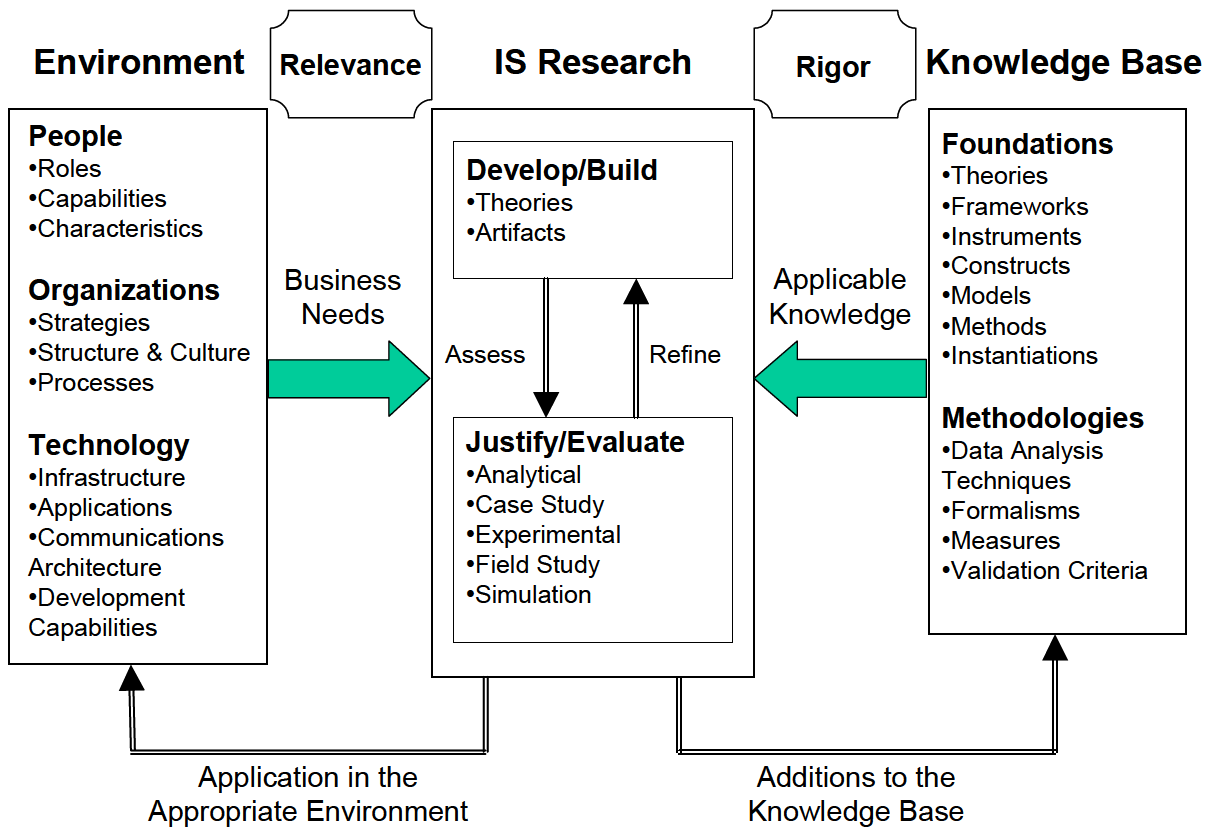
\includegraphics[width=\textwidth]{figures/hevner-research-framework.png}
    \caption{A framework for design science in the context of Information Technology \parencite{hevner2004design}}
    \label{fig:hevner-research-framework}
\end{figure}

A research methodology that fits such iterative process is design science. As defined by \textcite{hevner2004design} and illustrated in Figure \ref{fig:hevner-research-framework}, design science is a problem solving process that explores a relevant problem within an environment, iteratively measuring and refining the proposed solution according to the existing body of knowledge. The progress is made iteratively as the scope of the design of the artifact is expanded based on the discovery of available means, ends and constraints.

The use of a game-based calibration phase in this research influences how users behave during the emotion elitication process, e.g. body movement and facial expression. The movement of users directly impact the techniques for remote extraction of user signals during both the calibration phase and the emotion estimation phase, since those techniques are highly influenced by motion. The accuracy of those techniques regarding the remotely acquired signals is affected as well, which might invalidate the feasibility of remotely reading determined physiological and non-physiological signals required by the emotion estimaion model. The computer vision techniques, the model and the process associated with them must be continuously investigated and adapted to overcome those challenges. As a consequence, an iteractive cycle of development and research is required, as illustrated by Figure \ref{fig:hevner-generate-test}. In each iteration, a possible solution for the current set of problems is generated, rigourly tested and evaluated, producing information to guide the next iterations in the cycle. The set of design alternatives in this research are related to the identification of physiological and non-physiological signals to be used in the emotion detection process, how they can be elicitated with games in a calibration phase, which computer vision techniques can be employed to remotely acquire the signals and which machine learning model is able to map the information into emotional states. The set of constraints involve problems associated with users behaving naturally, e.g. laughing and moving the body during the procedure, use of non-specialized hardware, e.g. ordinary camera, accuracy and efficienty of the solution, among others.

\begin{figure}[h]
    \centering
    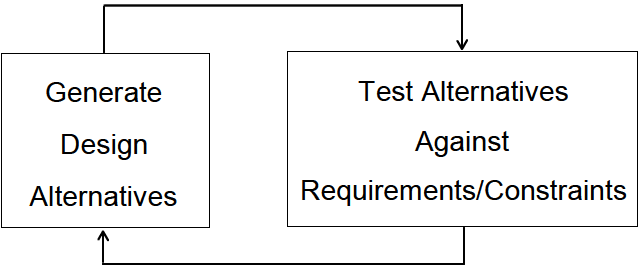
\includegraphics[width=0.6\textwidth]{figures/hevner-generate-test.png}
    \caption{The Generate/Test cycle. Adapted from \textcite{hevner2004design}}
    \label{fig:hevner-generate-test}
\end{figure}

%The aim of this research is to produce a utility tool, i.e. software, which is an artifact based on a model built on existing theories, which will be combined in a new and innovative way. Since the result of the research is a model, which will be built from different measurements to predict or infer a state, the present work stands on the positivism paradigm. Essentially this work will formulate a theory about how the variation of physiological signals relate to stress/boredom levels in the context of games and how it can be remotely detected. The involvement of humans in the process might relate to the social side of interpretivism, however the foundation of the work is still based on the analysis of physiological signals. Such signals and their patterns might be different for each person, however they are still ordered and regular under the human being perspective. As a consequence, they can be objectively observed, measured and analysed with a quantitative approach and hypothesis testing.

Design-science research requires the application of rigorous methods in both the construction and evaluation of the designed artifact \parencite{hevner2004design}. One of such evaluation methods is experimental research, which is the strategy used to build and validate the knowledge in this project. Such approach is composed of a set of research designs that use controlled testing and manipulation of variables in order to understand causal processes. The foundation of an experiment is to manipulate a variable (or a set of them) and measure any changes in other variables. It establishes the effect on a dependent variable, which is the focus of the research. The model being constructed in this research links the variations of user signals to stress/boredom levels in the context of games, hence there is a causal effect in the process since identified variations (cause) will precede changes in stress/boredom levels (effect). It progresses to the construction of a hypothesis where the cause will consistently lead to the same effect so the link between variations of signals and emotional levels can be inferred or predicted.

Each iteration in the design of the artifact will be constructed based on systematical investigation of existing theories, which will be refined and adapted to the context of the artifact. An experiment will validade the current artifact, producing information to guide the next iteration. The following section detail what is the current state of the project.

%\section{Research objectives}

%The objective of this research is to produce a method that is able to interpret remotely acquired signals from a person playing a game and detect his/her current emotional state regarding stress and boredom according to data previously obtained in a calibration phase. The model will be implemented in a software that uses a video feed to detect the person's emotional state.

%The current approaches used to obtain information from the players during games research inevitably affect the player's experience. They require the user to stop the game activity in order to share his/her current state, such as by answering a questionnaire. The frequency that such questionnaires are issued is also a concern. If performed too often, more information might be collected, but the data might contain noise caused by the frequent interruptions, e.g. player is more stressed/bored by the questionnaire interruptions than by the game itself. If performed too sparse, not enough information will be gathered from the player. A physical sensor attached to a player, on the contrary, allows a continuous monitoring process, however it is intrusive and might interfere with the player capacity to interact with the game. It might prevent the use or movement of specific parts of the body, for instance. Physical sensors also increase the chances of the player to behave differently as a side-effect of the monitoring process itself.

%A purely remote-based solution, as the one proposed by this research, enhances the tooling available to the games research community regarding investigation methods of stress and boredom. A games researcher will be able to increase the internal validity of his/her workflow by ensuring the player keeps the focus on the game without interruptions and by minimizing the side effects (and inconveniences) of physical monitoring. This research could also be deployed as a solution for game developer studios to automatically analyze hours of recorded gameplay and highlight the moments when boredom/stress levels changed significantly. As a complement the solution will be based on a single, ordinary camera and a software implementation, which eliminates the use of complex setups of physical sensors. It eases the investigation process and reduces costs.

\section{Current state of research}

As previously mentioned, this research is based on an interative problem solving strategy that involves the investigation and evaluation of different components. Figures \ref{fig:user-tailored-calibration} and \ref{fig:user-tailored-use}, in section \ref{sec:research-aim}, illustrate the combined use of the different parts involved in this project, which are all connected to the research objectives presented in section \ref{sec:contributions}. Figure \ref{fig:components-objectives} illustrates the correlation among the research objetives and the parts required to achieve the proposed research aim.

\begin{figure}[h]
    \centering
    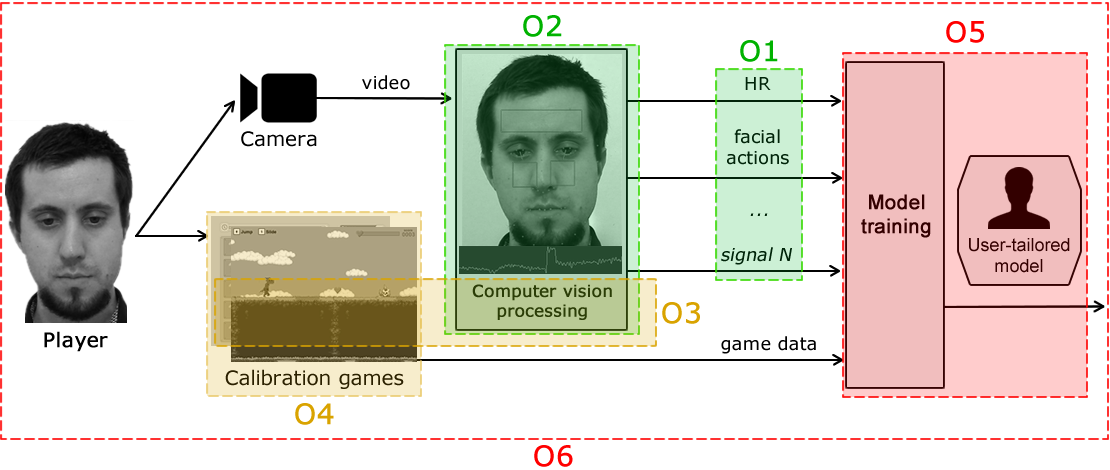
\includegraphics[width=\textwidth]{figures/components-objectives.png}
    \caption{Correlation among the research objetives and the parts required to achieve the proposed research aim. Red labels: not fulfilled yet. Yellow labels: partially fulfilled. Green labels: completely fulfilled.}
    \label{fig:components-objectives}
\end{figure}

Objectives marked in red and yellow are not fulfilled and partially fulfilled, respectively, so more investigation will be conducted regarding them. For information regarding future work, refer to chapter \ref{ch:closing}. Objectives marked in green have been completely fulfilled and the theories, concepts and results associated to each of them is documented in this thesis proposal. The chapters where such documentation and the associated objectives exist in this thesis proposal is presented in Figure \ref{fig:research-current-state}.

%The experiment design will be based on a within-subject approach \cite{lane2015online}. In such approach, all participants perform at all levels of the treatment and there are no control groups. It is the opposite of a between-subjects approach, where subjects are divided in more than one group that receive different treatments. In that approach there are special groups, called control groups, that receive no treatment. The comparison between the control groups and the treatment groups ensures internal validity. In the context of this research, physiological signals will be measured, so the division of subjects into more than one group poses a comparison problem. Each individual will inevitably differ from one another regarding physiological signals, such as variations in average HR during rest, for instance. When measuring HR, for instance, some subjects will have higher/lower HR mean than others, independent of the group they are in or the treatment they undergo. To counter that problem, the experiment will use a one-group posttest design \cite{kirk1982experimental}, as illustrated by Figure \ref{fig:experiment}. Using the first row as an example, subject $S_0$ played game $G_a$ as the first level of the treatment, followed by a post-test of that game ($PT_a$), then a rest period. In the second level of the treatment, the subject played game $G_b$, followed by a post-test of that game ($PT_b$), then another rest period. Finally in the third level of the treatment, the subject played game $G_c$ followed by a post-test of that game ($PT_c$).

%\begin{figure}[ht]
%    \centering
%    \includegraphics[scale=0.5]{imgs/experiment-design.png}
%    \caption{One-group posttest experiment design used in this research. $S_j$ represents the $j^{\text{th}}$ subject, $G_i$ represents a game of type $i$, $PT_i$ is the post-test for game $G_i$ and $rest$ is a resting period.}
%    \label{fig:experiment}
%\end{figure}

%By using a one-group posttest design, each individual will perform on all levels of the treatment (play a set of different games). The within-subjects approach ensures that the differences between subjects are not interfering in the comparison, since a subject is being compared to his/herself in the different levels of the treatment. Subjects are not being compared among each other. In essence, each subject is serving as his/her own control group. According to Kirk \cite{kirk1982experimental}, the one-group posttest design should only be used when the researcher knows the mean value of the independent variable when no treatment is in effect. Such information will be obtained during the resting periods of the experiment, where the baseline value for all measured signals can be established for each subject.

%The process of sampling a group of participants for each experiment will follow the convenience sampling approach, a non-probability sampling technique where participants are recruited because of their convenient accessibility/proximity to the researcher. Volunteers will be randomly recruited for each experiment. A probability sampling approach, where each individual of the population has an equal chance of being selected, would be ideal and would strength the external validity of the research. However the costs, logistics and time constraints associated with it makes such approach impractical in the context of this research.

Both objectives \textbf{O1} and \textbf{O2} have already been fulfilled. After the first literature review, the accomplishment of \textbf{O1} produced the identification of the main concepts, theories and signals associated with phychophysiological profile of users and their emotions. Chapters \ref{ch:literature-games}, \ref{ch:literature-physiological} and \ref{ch:literature-multifactorial} present the results of such literature review. The results of the literature review regarding objective \textbf{O2}, which focus on the identification of existing computer vision techniques to remotely extract signals from users, is presented in chapters \ref{ch:literature-face} and \ref{ch:literature-rppg}. The investigation also produced a publication regarding emotion detection and remote measurement of physiological signals \parencite{bevilacqua2015proposal}.

\begin{figure}[ht]
    \centering
    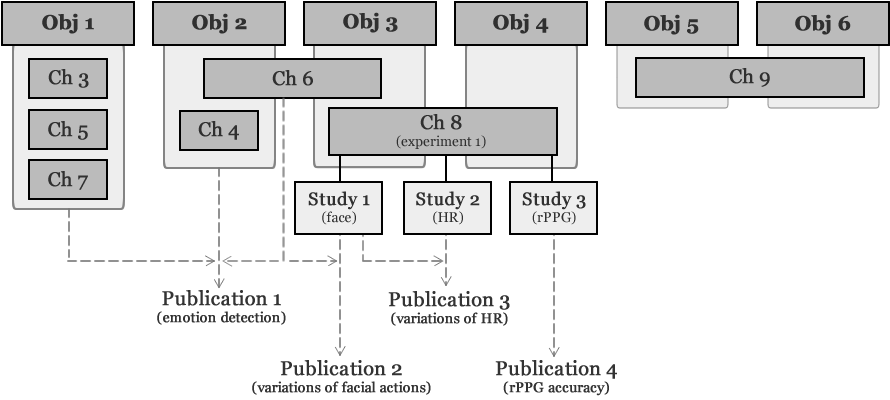
\includegraphics[width=\textwidth]{figures/research-current-state.png}
    \caption{The thesis proposal chapters coupled with the research objetives they cover.}
    \label{fig:research-current-state}
\end{figure}

Objective \textbf{O3} is being finalized. The aim of that objective, which is the investigation of feasibility, accuracy and challenges regarding the application of computer vision techniques within the context of games, was performed as an experiment. The experiment and the three studies conducted on the collected data are described and presented in chapter \ref{ch:experiment1}. Each one of those studies resulted in a publication, which present results regarding variations of facial actions \parencite{bevilacqua2016variations}, variations of heart rate \parencite{bevilacqua2017changes} and accuracy evaluation of the selected computer vision technique \parencite{bevilacqua2017accuracy}. The last two aforementioned publications were recently submitted for review. The main challenges regarding the application of the computer vision techniques within the context of games have already been identified. A publication \parencite{bevilacqua2017accuracy} and the literature review presented in chapter \ref{ch:literature-rppg} show the limitations of the computer vision technique when applied to contexts of games research involving natural behavior of users, e.g. head movement and face oclusion. A new study will be conducted to investigate ways to improve the computer vision technique to eliminate or mitigate such limitations.

Objective \textbf{O4} has been partially fulfilled. A pilot study, an experiment (described in chapter \ref{ch:experiment1}) and two publications \parencite{bevilacqua2016variations,bevilacqua2017changes} describe and validate the concept of calibration games. Up to the present moment, however, the variation of the signals produced by such calibration games have not been employed in any studies or experiments involving emotion detection, so its utility within the context of this research needs to be further investigated.

The future work planed to fullfil all research objectives is described in chapter \ref{ch:closing}.

\part{Literature review}
\chapter{Emotions theory}

%%%%%%%%%%%%%%%%%%%%%%%%%%%%%%%%%%%%%%%%%%%%%%%%%%%%%%%%%%%%%%%%%%%%%%%%%%%%%%%%%%%%%%%%%%%%%%%%%%%%%%%
\section{Russell's AV dimensional theory of emotions}
%%%%%%%%%%%%%%%%%%%%%%%%%%%%%%%%%%%%%%%%%%%%%%%%%%%%%%%%%%%%%%%%%%%%%%%%%%%%%%%%%%%%%%%%%%%%%%%%%%%%%%%

%%%%%%%%%%%%%%%%%%%%%%%%%%%%%%%%%%%%%%%%%%%%%%%%%%%%%%%%%%%%%%%%%%%%%%%%%%%%%%%%%%%%%%%%%%%%%%%%%%%%%%%
\section{Theory of flow}
%%%%%%%%%%%%%%%%%%%%%%%%%%%%%%%%%%%%%%%%%%%%%%%%%%%%%%%%%%%%%%%%%%%%%%%%%%%%%%%%%%%%%%%%%%%%%%%%%%%%%%%

\chapter{Games and emotions}

%%%%%%%%%%%%%%%%%%%%%%%%%%%%%%%%%%%%%%%%%%%%%%%%%%%%%%%%%%%%%%%%%%%%%%%%%%%%%%%%%%%%%%%%%%%%%%%%%%%%%%%
\section{Stress, boredom and flow}
%%%%%%%%%%%%%%%%%%%%%%%%%%%%%%%%%%%%%%%%%%%%%%%%%%%%%%%%%%%%%%%%%%%%%%%%%%%%%%%%%%%%%%%%%%%%%%%%%%%%%%%

%%%%%%%%%%%%%%%%%%%%%%%%%%%%%%%%%%%%%%%%%%%%%%%%%%%%%%%%%%%%%%%%%%%%%%%%%%%%%%%%%%%%%%%%%%%%%%%%%%%%%%%
\section{Immersion, engagement and sense of presence}
%%%%%%%%%%%%%%%%%%%%%%%%%%%%%%%%%%%%%%%%%%%%%%%%%%%%%%%%%%%%%%%%%%%%%%%%%%%%%%%%%%%%%%%%%%%%%%%%%%%%%%%

\chapter{Emotions and facial analysis}

The human face is a source of information and an important part of communication. Several elements connect this channel of information to emotional states, such as facial expressions and the activity of eyes and head \parencite{akakin2010spatiotemporal}. The analysis of such elements can convey information regarding emotional states, e.g. facial expressions are considered one of the most relevant features that can provide indication about emotional states \parencite{cowie2001emotion}.

\textcite{giannakakis2017stress} present a literature review focused on facial elements with value for detection of anxiety and stress, including the involvement of eyes (pupil size variations, gaze distribution, blinking rate), mouth (lips deformation, mouth activity) and head (head movement and velocity). Table \ref{table:stress-facial-features} lists all identified facial elements.

\begin{table}[h]
\begin{tabular}{lll}%
\toprule%
Head & Eyes & Mouth \\
\midrule
Head movement & Blink rate & Mouth shape \\
Skin color & Eyelid response & Lip deformation  \\
Hear rate (facial PPG) & Eye apperture & Lip corner puller \\
& Eyebrow movements & Lip corner depressor \\
& & Lip pressor \\
\midrule
Gaze & Pupil & \\
\midrule
Saccadic eye movements & Pupil size variation &  \\
Gaze spacial distribution & Pupil ratio variation &  \\
Gaze direction & &\\
\bottomrule%
\end{tabular}%
\caption{Categorization of facial elements connected with stress and anxiety \parencite{giannakakis2017stress}.}
\label{table:stress-facial-features}
\end{table}

There have been reports indicating that blinking increases with emotional arousal, including stress and anxiety levels \parencite{dinges2005optical}. Gaze direction, gaze congruence and the size of the gaze-cuing effect are also influenced by the level of anxiety or stress \parencite{staab2014influence}. Similarly mouth activity is influenced by conditions of stress, particularly lip movement \parencite{dinges2005optical} and asymmetric lip deformation \parencite{metaxas2004image}. Finally the frequency of mouth openenings has been measured as inversely proportional to the stress level under high cognitive load \parencite{liao2005decision}.

Regarding facial expressions, most of the works in the literature focus on detecting or classifing emotional states based on the six basic emotions proposed by \textcite{ekman1971constants}, i.e. happiness, surprise, sadness, fear, anger and disgust. The process usually involves the mapping of such emotion from facial Action Units (AU), which are indenfigied according to schemes such as the Facial Action Coding System (FACS) \parencite{ekman1977facial,cohn2007observer}. FACS aims to standardize the measurements of facial expression by defining highly regulated procedural techniques to detect facial actions/movements, which are decomposed into 46 different AUs anatomically related to facial muscles. When analyzed in defined contexts, such mapped actions can present a correlation between determined facial features and emotional states, e.g. stress and boredom.

The following sections present in more detail works related to face detection, including the analysis and relation to emotional states.

%%%%%%%%%%%%%%%%%%%%%%%%%%%%%%%%%%%%%%%%%%%%%%%%%%%%%%%%%%%%%%%%%%%%%%%%%%%%%%%%%%%%%%%%%%%%%%%%%%%%%%%
\section{Automated face detection}
%%%%%%%%%%%%%%%%%%%%%%%%%%%%%%%%%%%%%%%%%%%%%%%%%%%%%%%%%%%%%%%%%%%%%%%%%%%%%%%%%%%%%%%%%%%%%%%%%%%%%%%
The automated detection of faces is performed by techniques of Computer Vision, a subarea of Computer Graphics, whose aim is to make computers perceive the world in a similar way that humans do. Computer vision systems usually rely on image processing, artificial intelligence (e.g. machine learning) and decision making techniques to detect and classify objects from images or videos. A class of such objects is human faces, detected and analyzed by a process called facial alignment.

\begin{figure}[h]
    \centering
    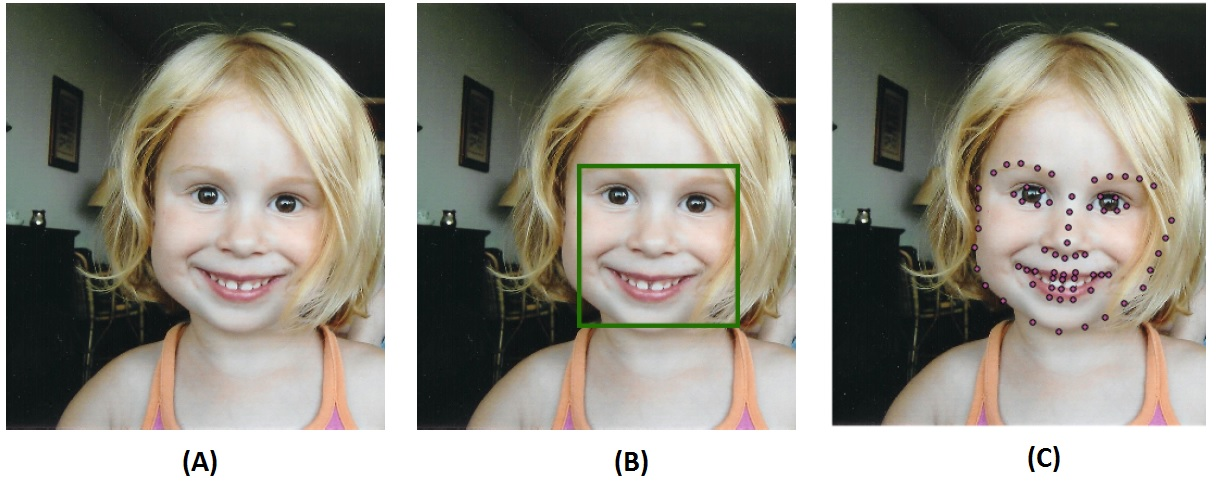
\includegraphics[width=\linewidth]{figures/face_alignment.jpg}
    \caption{Example of face alignment. (A) Input image. (B) Detected face. (C) Aligned face.}
    \label{fig:alignment}
\end{figure}

Facial alignment consists of identifying the position of specific features of the face, e.g. eye and nose, after the face has been detected in an image/video. Figure \ref{fig:alignment} demonstrates the process. This procedure is relevant in many different scenarios, for instance facial/expression recognition and pose estimation. Research has been conducted to create accurate and fast methods that can be used to perform face alignment under an ever growing set of challenging conditions, e.g. face movement combined with different lighting configurations.

Many methods have been proposed and a literature review shows that two basic approaches are widely used in alignment techniques: constrained local models and cascaded regression methods. Both approaches work on an image of a face contained within a rectangle obtained by a face detection algorithm, such as Viola \& Jones \parencite{viola2004robust}. The following sections describe each one of them, mentioning the most relevant techniques for facial alignment that are based on the approach being described.

\subsection{Constrained Local Model}

The Constrained Local Model (CLM) approach consists of locating a set of points on a target image, then applying a constrain to them. The constrain is usually based on a statistical shape model, which is obtained via training in a set of images featuring manually inserted landmarks. Since the shape model is statistical, the position of the points (landmarks) that it describes will always resemble a face, so proportions of lines and/or the distance among points will not be so different from a human face (at least not different from the ones found in the training set). Figure \ref{fig:clm-model-variation} illustrates the configuration of the shape model with different variations.

\begin{figure}[h]
    \centering
    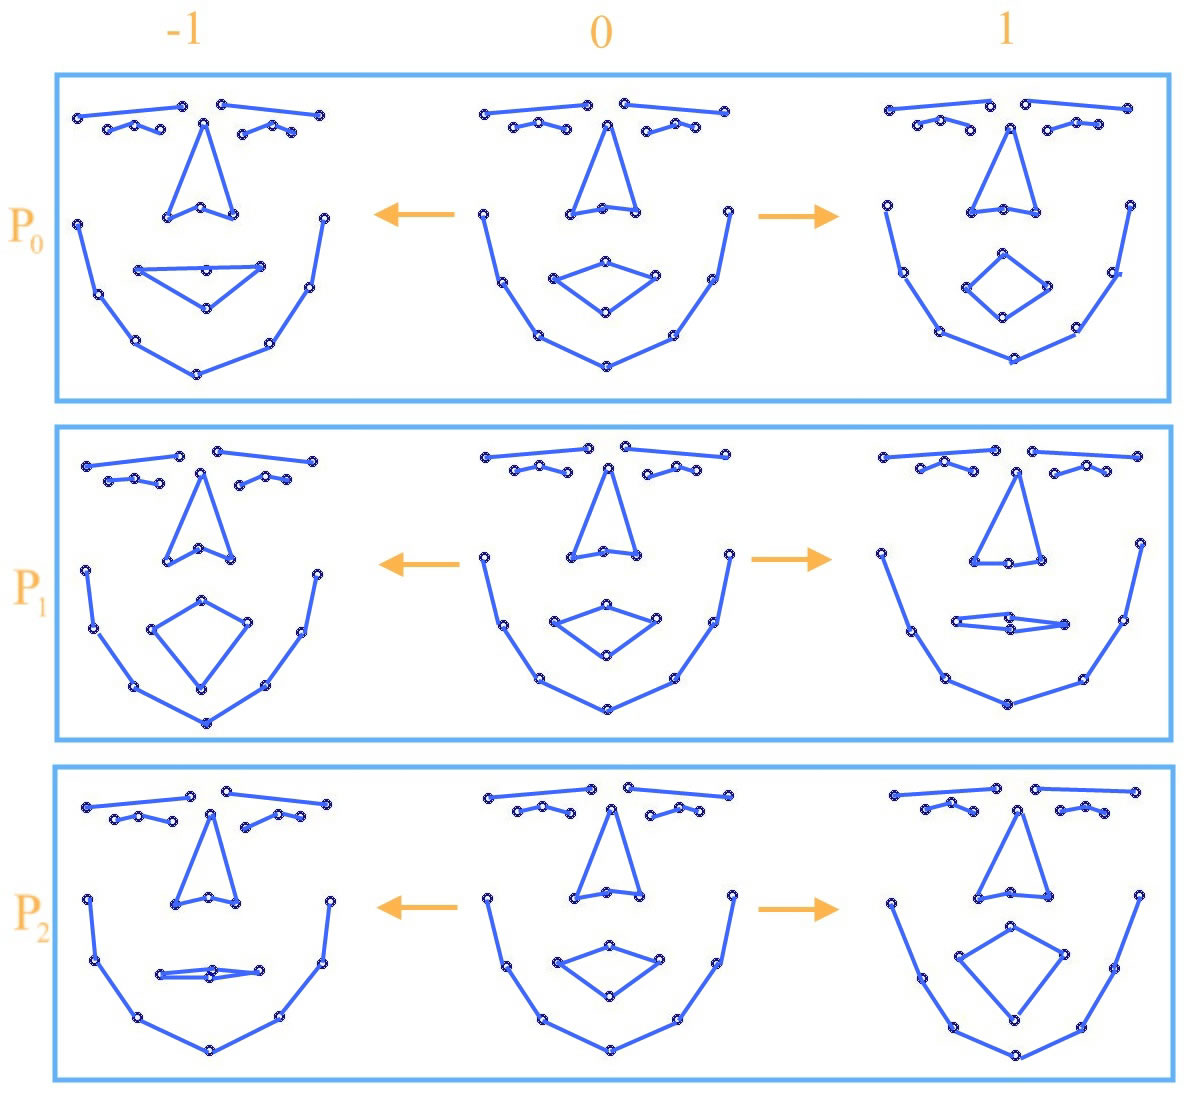
\includegraphics[width=0.6\linewidth]{figures/clm-model-variation.jpg}
    \caption{Configuration of the shape models with different variations \parencite{yu2010facial}.}
    \label{fig:clm-model-variation}
\end{figure}

Additionally to the shape model, there is a texture model that contains a set of patches (images) extracted from the training images by selecting the areas around the inserted landmarks. Those patches are used to guide the search procedure in the alignment process, which allows the technique to correctly identify the right model to properly align the face being analyzed. Figure \ref{fig:clm-patches} shows different shape models and their respective entries in the texture model.

The process of aligning a face is iterative and it starts by sampling points that are placed in the face image according to the current shape estimation of the face. In the first try, this estimation is usually the average face obtained from all training images. The area around the sampled points are extracted and used in a search to locate a set of similar patches in the texture model. The current shape estimation and the texture patches it locates are evaluated according to a cost function. As soon as the shape variation with the minimal cost is found, the process is repeated: new patches are sampled and searched against the texture model, the current estimation is adjusted and so on. Eventually the cost function will not produce a significantly different value from one iteration to another, which means the current estimation is the best match found.

\begin{figure}[h]
    \centering
    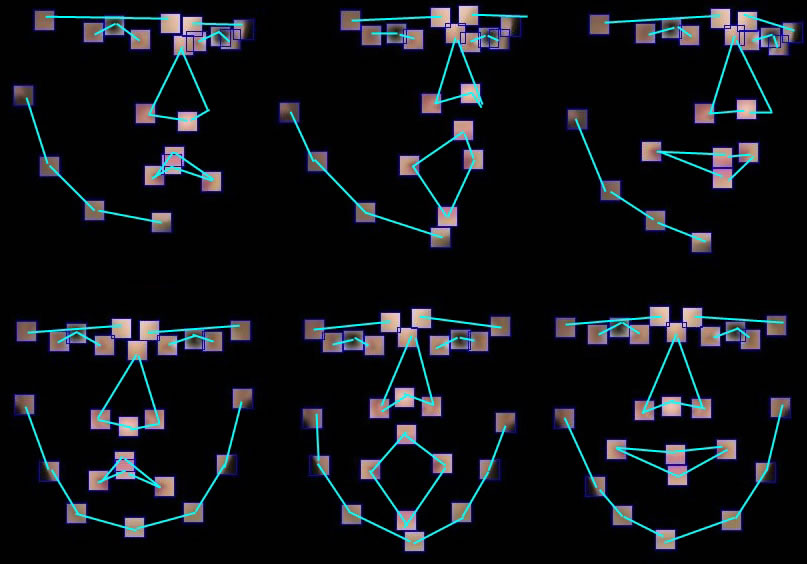
\includegraphics[width=0.6\linewidth]{figures/clm-patches.jpg}
    \caption{Shape models and their respective entries in the texture model \parencite{yu2010facial}.}
    \label{fig:clm-patches}
\end{figure}

Figure \ref{fig:clm-evolution} demonstrates the evolution of the technique as it iterates in an image. In Figure \ref{fig:clm-evolution}-(a), the mean shape is placed into the image and the patches are sampled around the (mistakenly) positioned landmarks. As the technique iterates ((b) and (c)), searched patches progressively induce changes in the current shape model, sampling more accurate patches. Eventually the technique converges to the aligned face, presented in Figure \ref{fig:clm-evolution}-(d).

\begin{figure}[h]
    \centering
    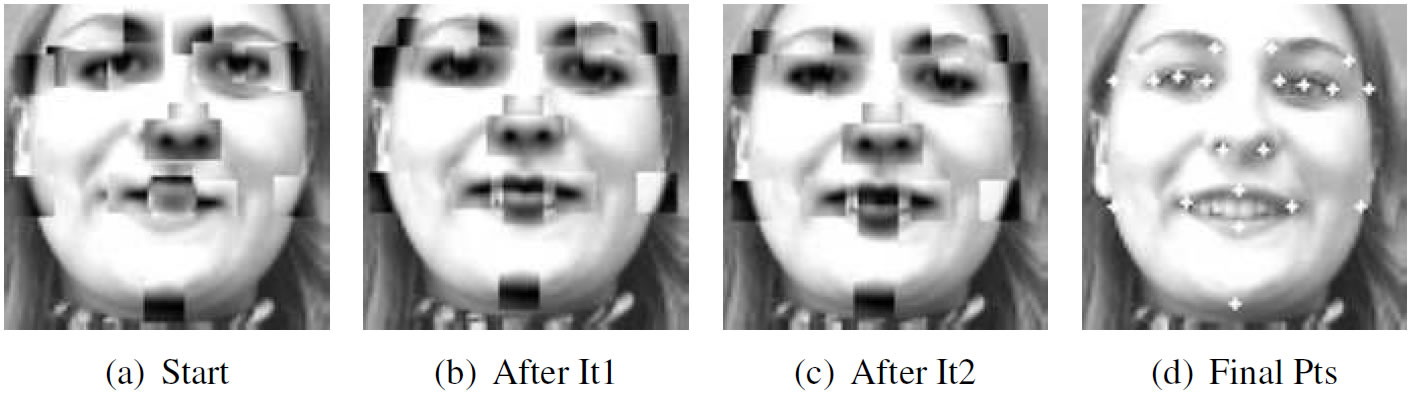
\includegraphics[width=\linewidth]{figures/clm-evolution.jpg}
    \caption{Iteration of CLM during the alignment of an image \parencite{cristinacce2006feature}.}
    \label{fig:clm-evolution}
\end{figure}

Two techniques that represent the CLM approach are the feature detection and tracking with constrained local models \parencite{cristinacce2006feature} and its 3D variation \parencite{baltruvsaitis20123d}, which uses 3D depth data to improve the process.

\subsection{Cascaded Regression}

The cascaded regression methods approach consists of using an initial guess shape that is progressively refined into the final answer (identification of key features in the image). This refinement is performed in a stage-by-stage manner (cascade) and the result of the current stage is used as the input for the next one. In each stage, the adjustment of the current shape (into the aligned result) is performed by a regression function, learnt via training. Early regressors in the cascade handle large variations in the shape, as opposed to the late ones, which focus on specific details. Each regressor extracts features from the image, which are then worked to produce variations in the current guess shape. The extracted features depend on the current shape and they are commonly referred as shape-indexed features.

The shape-indexed features are differences in pixel intensities. The calculation of a shape-indexed feature involves the selection of a few pixels and the subtraction of their intensities. The way those pixels are selected is usually different for each of the cascaded-regression techniques. Figure \ref{fig:shape-indexed} illustrates an example of selection of a few pixels for three particular landmarks. The landmark on the top-right (gray circle) highlights the selected pixels that will be used. The difference of intensities among those pixels will define this particular shape-indexed local feature. The shape-indexed local features are used in a decision process in each step (cascade), as illustrated by Figure \ref{fig:regressor-steps}. Usually the initial guess shape is the mean shape of the training set. This guess is used to calculate the current set of shape-indexed features to be extracted, which then guides the variation applied to the current shape. The variation to be applied is usually chosen based on the result of a cost function, which selects a variation that minimizes the distance between the current guess and the supposed aligned face. As the process repeats itself, different shape-indexed features are selected, a new variation is calculated and so on. Eventually the current shape will converge and it will represent the alignment for the face being analyzed (final shape estimation).

\begin{figure}[h]
    \centering
    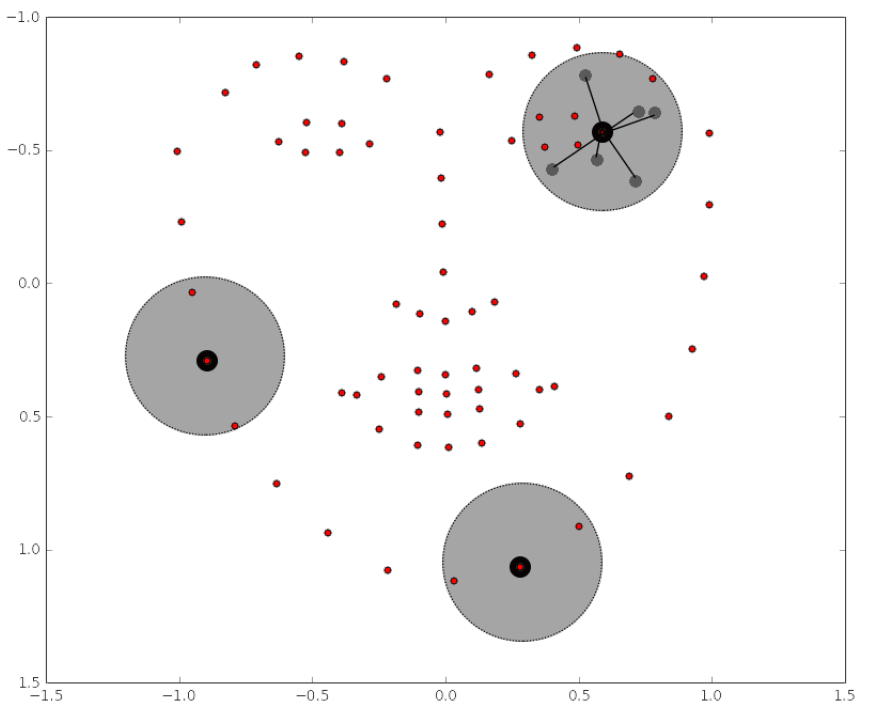
\includegraphics[width=0.6\linewidth]{figures/shape-indexed.png}
    \caption{Pixels used in the calculation of a shape-indexed feature \parencite{maris2015}.}
    \label{fig:shape-indexed}
\end{figure}

\begin{figure}[h]
    \centering
    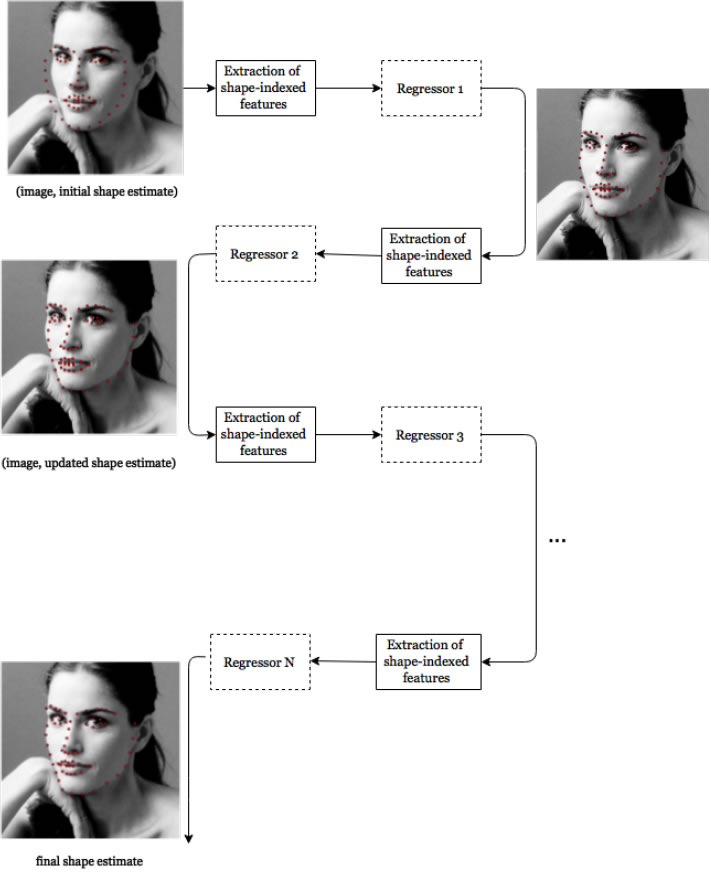
\includegraphics[width=0.9\linewidth]{figures/cascade-explanation.jpg}
    \caption{Estimation of face shape with regressors in a set of stages \parencite{maris2015}.}
    \label{fig:regressor-steps}
\end{figure}

Different variations are used to handle the training, the extraction of features and the way the regression is performed. The technique of face alignment with Ensemble of Regression Trees (ERT) \parencite{kazemi2014one}, for instance, estimates the face's landmarks by inputting the regressors with a sparse subset of pixels intensities, which is calculated with a prior probability on the distance of the pixels. The Supervised Descent Method (SDM) \parencite{xiong2013supervised}, on the other hand, extracts SIFT features from the current shape estimation and it converges the shape by solving a series of linear least square problems. The approach via regression of Local Binary Features (LBF) \parencite{ren2014face} proposes the use of a set of local binary features (opposed to a global view of the face) combined with a locality principle for learning and processing such features independently. Finally the face alignment by Explicit Shape Regression (ESR) \parencite{cao2014face} trains the regressors by explicitly minimizing the alignment error over training data, so all facial landmarks are regressed jointly.
%The regressors work by progressively inferring the shape, so the early regressors in the cascade handle large shape variations (ensures robustness) while later regressors focus on the small and subtle variations (ensures accuracy).

%%%%%%%%%%%%%%%%%%%%%%%%%%%%%%%%%%%%%%%%%%%%%%%%%%%%%%%%%%%%%%%%%%%%%%%%%%%%%%%%%%%%%%%%%%%%%%%%%%%%%%%
\section{Facial-based emotion prediction}
%%%%%%%%%%%%%%%%%%%%%%%%%%%%%%%%%%%%%%%%%%%%%%%%%%%%%%%%%%%%%%%%%%%%%%%%%%%%%%%%%%%%%%%%%%%%%%%%%%%%%%%

\subsection{Detection based on facial expressions}

\textcite{bailenson2008real} present a machine learning model built from the previously mentioned idea of combining facial expressions and physiological signals to predict emotion (sadness or amusement). Subjects are recorded by a camera while they watched a video composed of segments of different emotions (neutral, amusement and sadness). Additionally 15 physiological signals are also recorded, among them HR, skin conductance level and finger temperature. The video recordings are annotated by professional coders; the annotated video frames are used in conjunction with the physiological signals to produce the predicting model. The authors compare the performance of models built from different data sources, such as the data from all subjects (general model), from the female/male population (gender-specific model) or from a single individual (person-specific model). The model performs better when categorizing emotions instead of predicting its intensities and when detecting amusement instead of sadness. Additionally the pinserson-specific model outperformes the other two variations, suggesting that a person-tailored model might be more effective in identifying features (even the more subtle ones) than a general-purpose model. The results also state that a model built from a combination of facial and physiological information is more efficient than a model built with either one alone.

\textcite{grafsgaard2013automatically} present an experiment where only facial expression information is used. The experiment is an automated analysis of FA during computer mediated tutoring sessions among students. Subjects and tutors interact through a tutoring software related to computer programming, while subjects are recorded. After each session, subjects answer a questionnaire related to measurements of cognitive load and engagement. The recordings are analyzed in an automated way with manual verification of the results. A predictive model is constructed using the questionnaire answers and the recording analysis, which results in correlations of FA and emotional states. The authors compare their findings against other research, which differ significantly. For instance, brow lowering has been correlated with confusion in previous work, however the authors found that it was a positive predictor of student frustration in the context of their experiment. Such difference in results is expected due to the variational nature of facial expressions among different individuals and contexts, however it underlines the complexity of correlating facial features and emotions. \textcite{heylen2005facial} also present a similar investigation in a pilot experiment of a tutoring session related to the application of subcutaneous injection. Students interact with a virtual patient while using a physical haptic device to administrate an injection. The recordings of the students are analyzed by the researchers to make annotations of the expressions based on their own interpretation of the context. The researchers use a compilation of literature components to guide the evaluation of the collected data. As the authors point out, a variety of expressions occur, but most of the time students remain with a neutral facial expression. The annotated features are (ordered from most to less frequent): smile (total 22), raise eyebrows (11), pull down mouth corners (2) and frown (1).

%As opposed to previously mentioned works, our approach consists of using induced boring to stressful mechanics in games to produce variations in the emotional state of participants. Our experiment has a linear progression from a boring to a stressful state that should be perceived by the subjects. We believe such configuration gives our experiment a novel approach for the exploration of facial actions and HR regarding their connection to emotional states, since we can categorize information according to the induced (and theoretically known) emotional states. To the best of our knowledge, this is the first experiment where games with linear boring-to-stressful progression are used to deliberately induce emotional reactions.

\subsection{Detection based on facial movement}

\textcite{giannakakis2017stress} present an approach for detection of stress/anxiety based on eye blink, mouth/head movements and HR.

\begin{figure}[h]
    \centering
    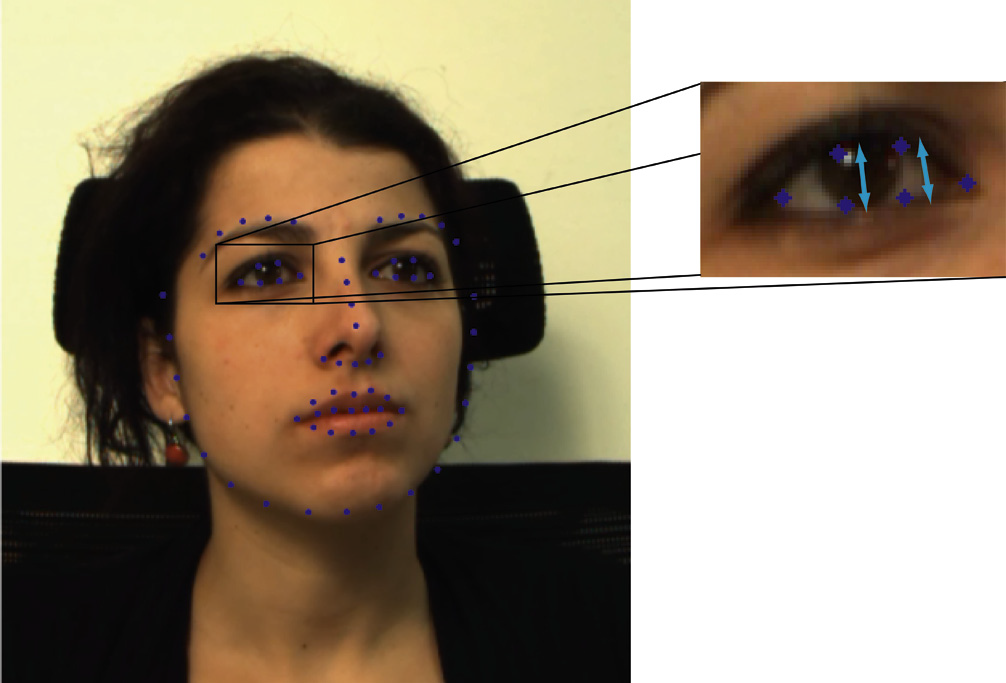
\includegraphics[width=\linewidth]{figures/giannakakis2017stress-eye.png}
    \caption{Highlight of average distance calculation regarding eye apperture \parencite{giannakakis2017stress}.}
    \label{fig:distance-samara}
\end{figure}

\textcite{samara2016sensing} use Euclidian distance among face points to train an SVM model to detect expressions.

\begin{figure}[h]
    \centering
    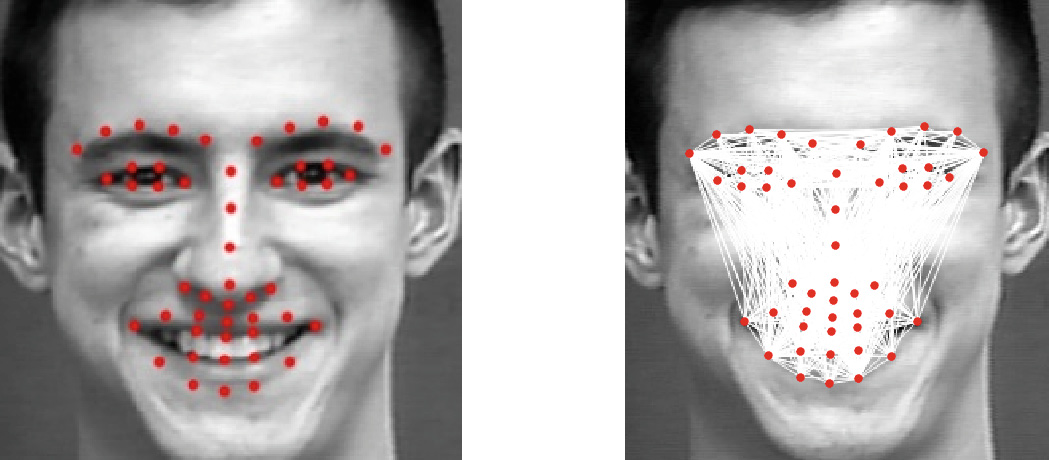
\includegraphics[width=\linewidth]{figures/samara2016sensing-distances.png}
    \caption{Distance-based facial feature descriptors \parencite{samara2016sensing}.}
    \label{fig:distance-samara}
\end{figure}

\chapter{Emotions and physiological signals}

%%%%%%%%%%%%%%%%%%%%%%%%%%%%%%%%%%%%%%%%%%%%%%%%%%%%%%%%%%%%%%%%%%%%%%%%%%%%%%%%%%%%%%%%%%%%%%%%%%%%%%%
\section{Introduction}
%%%%%%%%%%%%%%%%%%%%%%%%%%%%%%%%%%%%%%%%%%%%%%%%%%%%%%%%%%%%%%%%%%%%%%%%%%%%%%%%%%%%%%%%%%%%%%%%%%%%%%%

%%%%%%%%%%%%%%%%%%%%%%%%%%%%%%%%%%%%%%%%%%%%%%%%%%%%%%%%%%%%%%%%%%%%%%%%%%%%%%%%%%%%%%%%%%%%%%%%%%%%%%%
\section{Physiology of heart rate}
%%%%%%%%%%%%%%%%%%%%%%%%%%%%%%%%%%%%%%%%%%%%%%%%%%%%%%%%%%%%%%%%%%%%%%%%%%%%%%%%%%%%%%%%%%%%%%%%%%%%%%%

%%%%%%%%%%%%%%%%%%%%%%%%%%%%%%%%%%%%%%%%%%%%%%%%%%%%%%%%%%%%%%%%%%%%%%%%%%%%%%%%%%%%%%%%%%%%%%%%%%%%%%%
\section{Heart rate, stress and frustration}
%%%%%%%%%%%%%%%%%%%%%%%%%%%%%%%%%%%%%%%%%%%%%%%%%%%%%%%%%%%%%%%%%%%%%%%%%%%%%%%%%%%%%%%%%%%%%%%%%%%%%%%

\chapter{Remote photoplethysmography}
\label{ch:literature-rppg}

Photoplethysmography (PPG) is a technique commonly used to measure HR based on the variations of light absortion in the human skin. The pressure of the cardiac activity causes the blood vessels to change volume and light absorbtion rate because of the levels of oxigen in the blood flow. Such differences make the light absorption on the skin surface change accordingly. PPG is a time-varying signal resulted from such differences in the light absorption in live human tissue, which can be processed to calculate the HR. The process is illustrated in Figure \ref{fig:ppg}. The employment of PPG requires a physical sensor, e.g. finger pulse oximeter, in order to be performed.

\begin{figure}[h]
\centering
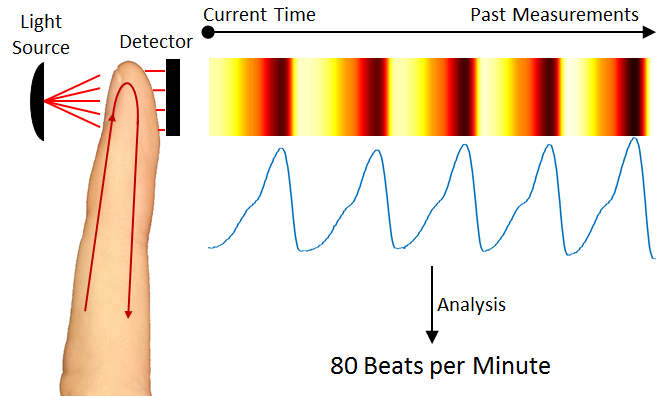
\includegraphics[width=0.7\linewidth]{figures/ppg.png}
\caption{General structure of a physical photoplethysmographic system. Adapted from \textcite{chwyl2016statistical}.}
\label{fig:ppg}
\end{figure}

Further research on PPG \parencite{mcduff2015survey} evolved the technique to allow it to be performed remotely based on the analysis of a video of a person. The remote approach is commonly refered in the literature as remote photoplethysmography (rPPG)  \parencite{allen2007photoplethysmography}. Such improvement removed the requirement of a physical sensor or any physical contact for the estimation of HR and its derivates. A literature review shows the existence of a variety of different rPPG approaches, including thermal-, image-, and movement-based ones \parencite{kranjec2014non, Sereevoravitgul}. The following sections present the common structure of an rPPG technique, a survey of existing rPPG techniques and information regarding accuracy and limitations of such technology.

%rPPG-based methods for HR measurement are tools that can be used by the HCI community, particularly in games research.

%The use of physiological signals to infer information about users is a recurrent research topic \parencite{kivikangas2011review,jerritta2011physiological, kukolja2014comparative}. However the methods employed to obtain such signals are commonly based on physical contact, e.g. ECG, and few initiatives have been carried out relying on non-contact approaches, e.g. rPPG. In the computer vision domain, on the other hand, an increasing number of works is concerned with creating new (or improving already existing) techniques for rPPG. To provide an introduction for readers unfamiliar with rPPG, we introduce its general structure and the core techniques in the field. Additionally we present works involving physiological signals, in particular HR, and game-related materials commonly used for detection of emotional states of users.

%%%%%%%%%%%%%%%%%%%%%%%%%%%%%%%%%%%%%%%%%%%%%%%%%%%%%%%%%%%%%%%%%%%%%%%%%%%%%%%%%%%%%%%%%%%%%%%%%%%%%%%
\section{Structure of the technique}
\label{s:literature-rppg-structure}
%%%%%%%%%%%%%%%%%%%%%%%%%%%%%%%%%%%%%%%%%%%%%%%%%%%%%%%%%%%%%%%%%%%%%%%%%%%%%%%%%%%%%%%%%%%%%%%%%%%%%%%

There exist initiatives to classify \parencite{rouast2016remote, mcduff2015survey} and formally model the algorithmic principles \parencite{Wang_2016algorithmic} of rPPG techniques. In that light, \textcite{rouast2016remote} propose a general algorithm framework composed of three phases that are common to all rPPG techniques (see Figure \ref{fig:rppg}): signal extraction, signal estimation and heart rate estimation.

\begin{figure}
\centering
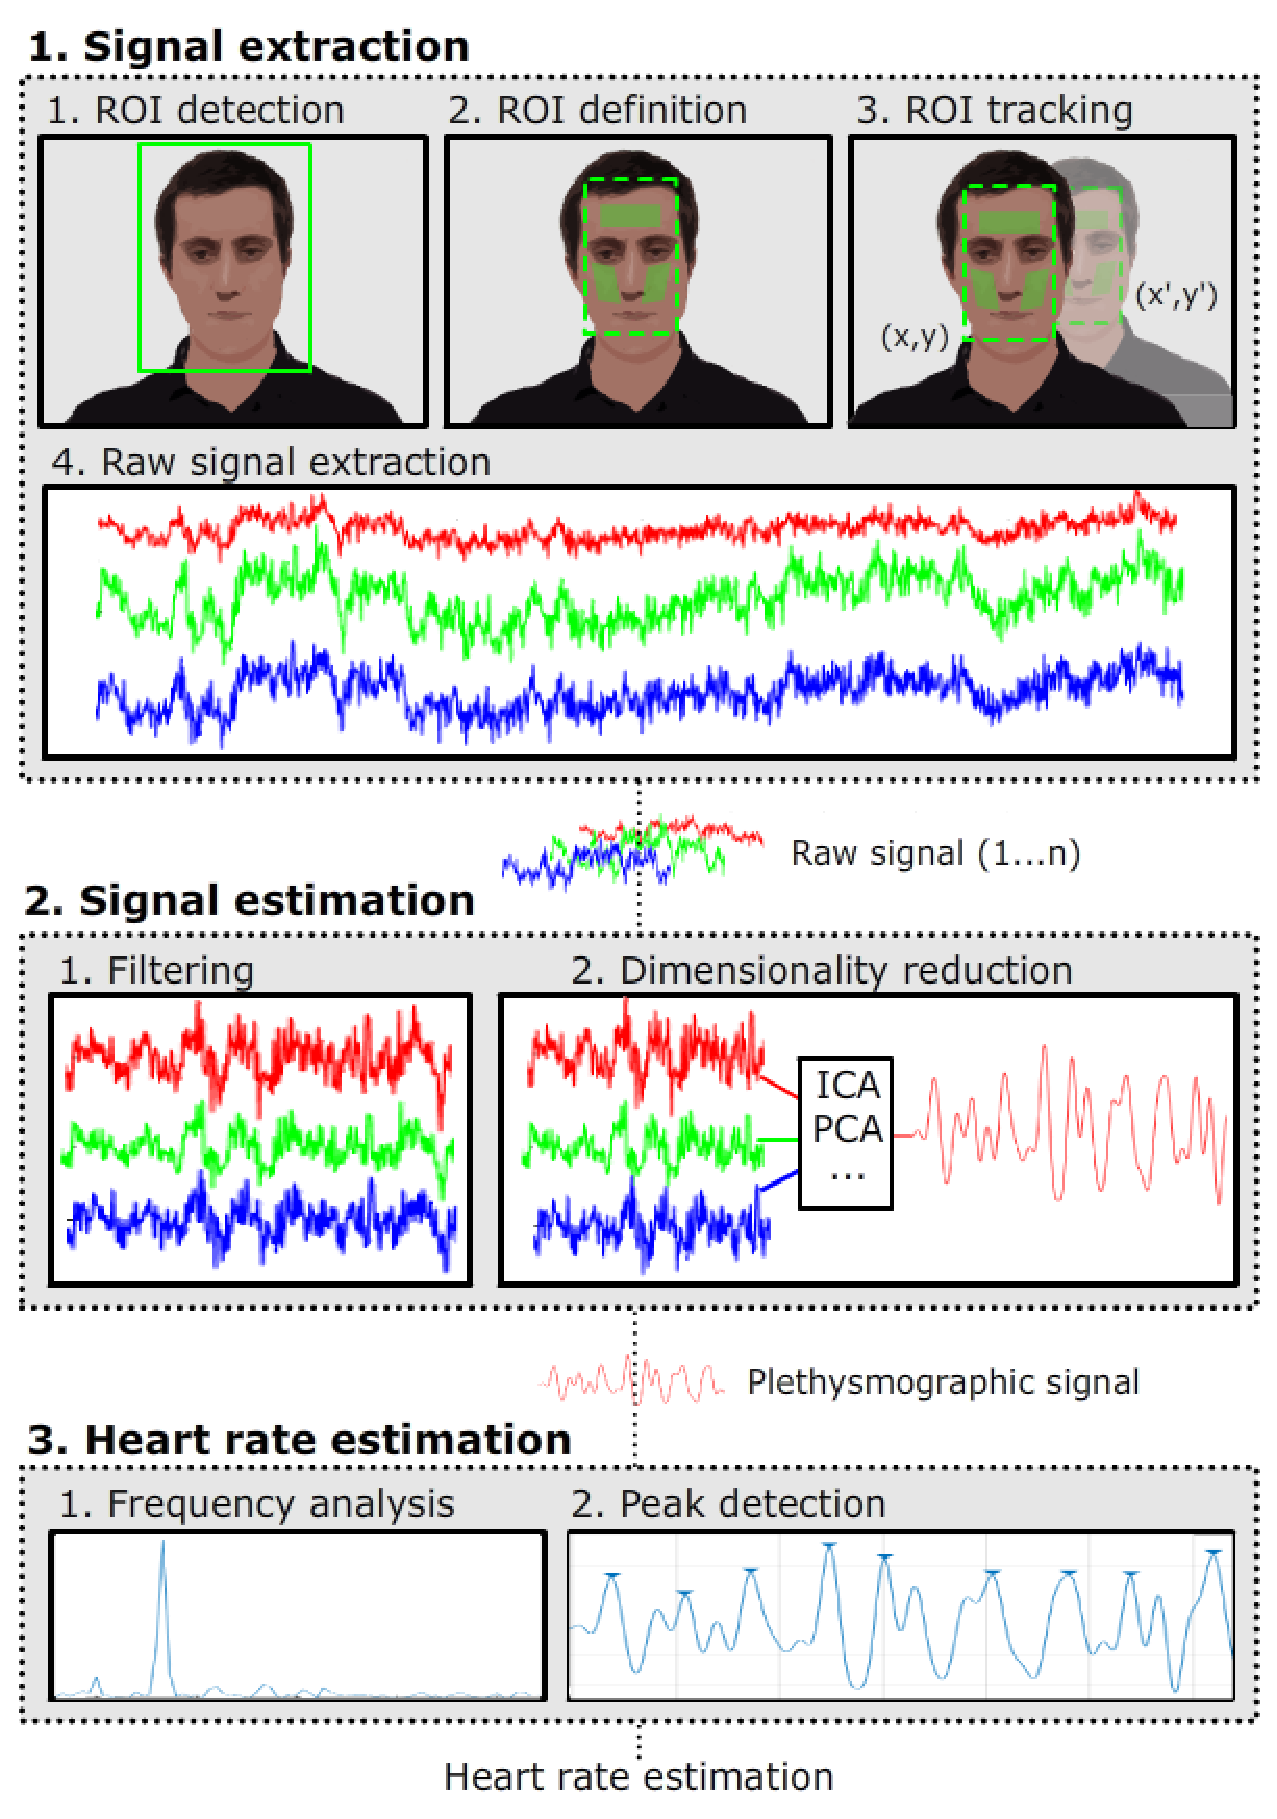
\includegraphics[width=0.9\linewidth]{figures/general-rppg}
\caption{General algorithm framework common to all rPPG techniques. Adapted from \textcite{rouast2016remote}.}
\label{fig:rppg}
\end{figure}

\subsection{Signal extraction}

The signal extraction phase extracts a set of raw signals from a video. Step 1 relates to the detection of a region of interest (ROI), which is an area of the video that usually contains the face of the subject. Approaches commonly used for this step are the algorithm of Viola\&Jones (VJ) \parencite{ViolaJones}, a machine learning based approach to classifying faces, Active Appearance Models (AMM) \parencite{EdwardsAAM} and facial landmark detectors. %\parencite{saragih2011deformable,martinez2013local}.

In step 2 (ROI definition) the parts of the ROI to be used for the signal extraction are defined. Approaches commonly employed include the use of whole ROI (usually the bounding box returned by VJ, which is likely to contain background pixels along with the facial pixels), a part of the ROI (e.g. 60\% of the bounding box width) or specially defined areas (e.g. forehead, cheeks or shapes defined by facial landmark points).

Step 3 (ROI tracking) deals with the process of tracking the defined ROI area over the duration of the video. Ideally the PPG signal should be extracted from the pixels belonging to the same skin region over time. This is unlikely to happen due to subject motion, be it voluntary or not (subjects will present movement that influences the ROI even when still \parencite{poh2010non}). A common approach for this step is the re-detection of the ROI for each frame, which is computationally suboptimal and still prone to noise. Detection algorithms, e.g. VJ, are not likely to be exact, so results between consecutive frames might be slightly different, which causes fluctuation in the defined ROI. More elaborated approaches avoid the costly frame-by-frame re-detection procedure (and its fluctuations) by updating an already detected ROI in subsequent frames. The update is based on movement information obtained from tracking algorithms applied to features/points within the ROI. %Examples of such algorithms are Good Features to Track, Kanade-Lucas-Tomasi (KLT), Speeded Up Robust Features (SURF), Kernel-based Object Tracking and tracking-by-detection with kernels.

Finally in step 4 (raw signal extraction) a raw (untreated) signal is extracted. It is a time-varying signal whose points/samples are obtained from the content of the defined ROI in each frame of the video. One common approach used to extract the signal is based on colors, e.g. average of the values of the pixels of each channel (R, G and B) over time produces the raw signal. Another approach is based on the movement of the head, which is a mechanical reaction to the blood flow in the aorta. Feature points within the defined ROI are tracked over time by a tracking algorithm and the horizontal and/or vertical variations in the trajectory of the points produce the raw signal. The signal extraction phase can result in multiples raw signals, which are dependent on the approach applied. A color-based approach, for instance, might result in three raw signals, one for each color channel (RGB).

\subsection{Signal estimation}

The raw signals are filtered and combined to produce a single estimated plethysmographic signal. The filtering step aims to remove unwanted noise from the raw signal, which could be caused by the capturing device (e.g. camera noise), subject movement, changes in illumination, etc. The raw signal is usually normalized (subtracted by its mean and divided by its standard deviation) first. The commonly used filters are based on high/low pass, such as bandpass, moving average window and detrending based on Smoothness Priors Approach (SPA) \parencite{eleuteri2012efficient}. Since the feasible frequencies for the HR band are known, filters are usually configured to eliminate frequencies outside that band, e.g. cutoff frequencies of [0.7 Hz, 4.0 Hz], which eliminates from the raw signal frequencies outside the [42 bpm, 240 bpm] interval.

In the dimensionality reduction step, the raw signal is used to estimate the plethysmographic signal, i.e. the one containing the HR. As previously mentioned, depending on the approach used for the raw signal extraction, one or more raw signals might be available for use in the estimation. One approach for the estimation is to simply choose one of the raw PPG signals as the estimated plethysmographic signal, e.g. the raw signal extracted from the G channel. Such choice is acceptable since the plethysmographic signal is known to be stronger in the green channel of an RGB video \parencite{verkruysse2008remote}, however it is more likely to contain noise since a raw (untreated) component is being used. Another approach relies on Blind Source Separation (BSS) methods, which tries to mitigate noise by assuming the estimated plethysmographic signal is a linear combination of the raw signals. Independent Component Analysis (ICA) \parencite{hyvarinen2000independent} and Principal Component Analysis (PCA) \parencite{jolliffe2002principal} are common BSS algorithms used to find the weight that each raw signal has in the linear combination to produce the estimated plethysmographic signal. Finally another approach assumes fixed weights for the linear combination, which are derived from models of skin illumination, for instance.

\subsection{Heart rate estimation}

Finally the estimated plethysmographic signal is analyzed and the HR is extracted. There are two steps in this phase, frequency analysis and peak detection, however only a single one of them is usually performed. In the frequency analysis step, approaches include Continuous Wavelet Transform (CWT) used to construct a time-frequency representation of the plethysmographic signal, and Fourier Transform to analyze the signal in the frequency domain. Regarding the later, the estimated plethysmographic signal is assumed to contain a distinct periodicity (the HR). As a result, when converted into the frequency domain via Fast Fourier Transform (FFT), for instance, the signal should present a high spectral power associated with the frequency of such distinct periodicity. As a consequence, the index of the frequency with the highest peak in the power spectra in the frequency domain corresponds to the HR.

In the peak detection step, however, the signal is not converted into the frequency domain, instead it is interpolated and peaks are detected (usually with a local maxima algorithm). The distances among the peaks correspond to the inter-beat interval (IBI), which is then used to calculate the HR (as $60/\overline{IBI}$) and/or the heart rate variability (HRV).

%%%%%%%%%%%%%%%%%%%%%%%%%%%%%%%%%%%%%%%%%%%%%%%%%%%%%%%%%%%%%%%%%%%%%%%%%%%%%%%%%%%%%%%%%%%%%%%%%%%%%%%
\section{Consolidated techniques}
\label{s:literature-rppg-techniques}
%%%%%%%%%%%%%%%%%%%%%%%%%%%%%%%%%%%%%%%%%%%%%%%%%%%%%%%%%%%%%%%%%%%%%%%%%%%%%%%%%%%%%%%%%%%%%%%%%%%%%%%

The previously described general algorithm framework for rPPG techniques illustrates the wide range of variations possible by different combinations of approaches within each step of the process. Early initiatives regarding rPPG, for instance, used manually detected/defined ROI, few or no use of signal filtering and signal extraction based on the average of image brightness \parencite{takano2007heart} or colors \parencite{verkruysse2008remote}.
%Additionally the authors presented findings regarding the process: PPG signal is stronger in the green channel of an RGB video, which is aligned with the fact that hemoglobin absorbs green light better; each pixel in the ROI contributes to the HR signal detection, which implies that the selection/size of the ROI is not critical for HR determination; lighter areas in the video often feature a higher pulse signal; and the PPG signal obtained from facial regions, specially the forehead, are stronger than other body parts.

The work of \textcite{poh2010non} was the first in the field to rely on BSS. Figure \ref{fig:poh} illustrates the proposed approach. The authors extracted the signal using automatic definition/tracking of the ROI (based on 60\% width of a VJ bounding box) and the average of the color channels. The three raw signals (derived from R, G and B) were filtered, detrended and decomposed using ICA. The second component generated by ICA was interpolated and a custom algorithm detected peaks to identify the HR. The authors further improved the technique by selecting the ICA component whose power spectrum contained the highest peak \parencite{poh2011advancements} and by incorporating alternate frequency bands (i.e. orange and cyan) into the extraction phase \parencite{mcduff2014improvements}.

\begin{figure}
\centering
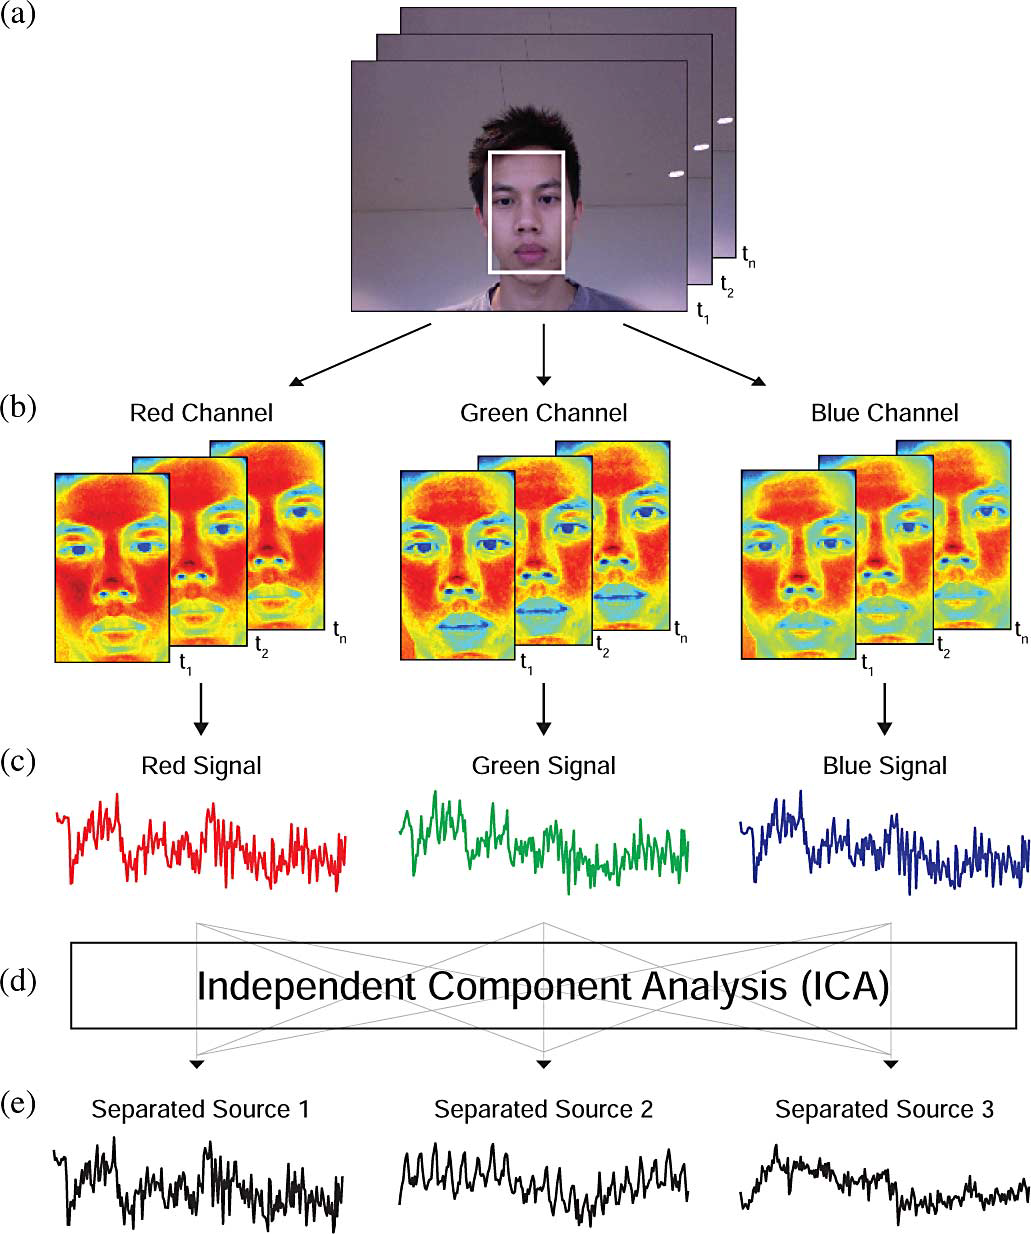
\includegraphics[width=0.7\linewidth]{figures/poh.png}
\caption{rPPG approach based on ICA \parencite{poh2010non}.}
\label{fig:poh}
\end{figure}

\textcite{Datcu_2013} present a similar approach, however using AAM to segment the face of the subject into ROIs. \textcite{li2014remote} also use a different ROI, based on facial landmarks, and a combination of additional steps to mitigate noise caused by illumination, motion and facial expressions by removing signal outliers. \textcite{bousefsaf2013continuous} propose a variation of the previously described approaches, using a skin detection procedure to select pixels in the signal extraction phase. Additionally CWT is used in the signal estimation phase instead of the commonly used FFT, which is pointed by authors as more suitable for rapid changes in frequencies in time. As a consequence, the authors were able to detect the instantaneous HR (iHR) and significantly reduce the waiting time for the detection of HR measurements.

%used a digital version of the Stroop test and a video of a subject (captured by a webcam) to calculate HR and HRV to detect stress. A combination of HR, HRV and $HRV_{HF}$ is used to estimate the stress state. The resulting stress state curve tends to decrease during the rest period and increase during stress sessions (as the HR measurements), in accordance with previously mentioned works; additionally self-reported answers from questionnaires present significant differences of stress level in the rest and in the stress sessions as well, which confirms that remote reading and processing of HR as an input signal is able to relate with the real emotional state of an user. The detection mechanism, however, is purely based on the assumption that stress increases the HR mean. Both HR and HRV are averaged and interpolated within a time span (27 seconds) and the resulting wave produced from that calculation is said to be the stress level. Such wave might describe stress levels, since it matched variations of electrodermal response (EDR) data recorded using a skin conductance sensors, which is an indicator of stress, but the wave can also be seen as a simple representation of the HR and HRV variations, not stress itself.

Different approaches that are not based on the average of colors of the face can also be found in the literature. Those techniques use knowledge of the color vector of the different components to perform  the signal extraction. \textcite{Wang_2016novel} focus on the definition of a plane orthogonal to the skin-tone, ignoring pixels outside the subspace of skin pixels in the signal estimation phase. Similarly \textcite{de_Haan_2013} also use a skin model to generate a chrominance-based PPG signal, which is calculated as a combination of the intensities of the color channels in the video instead of their average. Those techniques aim to be more resilient than BSS-based techniques regarding motion noise. \textcite{6619284} are the first to completely move away from color-based initiatives and perform the signal extraction based on head movements. \textcite{Irani} further improved the technique by using a moving average filter applied to the trajectory of the feature points being tracked to remove the noise produced by other sources of motion, e.g. respiratory activity.
%Yun et al. \parencite{yun2009game}, on the other hand, demonstrated that changes in HR cause variation of temperature in the lower area of the forehead, which can be measured by a thermal imaging camera and used to infer stress state. The analysis performed by the authors was based on the variations of temperature in such lower area of the forehead, which differs from the color averaging approach previously described and used by other authors. The results, however, highlight that the region is affected by stress activities, which confirms the findings of \parencite{Datcu_2013}, \parencite{Sereevoravitgul} and \parencite{verkruysse2008remote} that point the forehead area as being more prone for remote readings.

The different settings in each phase of an rPPG technique result in a trade-off between advantages and disadvantages. Estimation based on head movement, e.g. \textcite{6619284}, does not rely on previous knowledge about colors nor requires visible skin area to work. However it is outperformed by other methods when subjects are not completely still \parencite{li2014remote} since it is significantly affected by subject motion. Techniques based on pre-defined skin-tone models, e.g. \textcite{Wang_2016novel,de_Haan_2013}, better adapt to changes in illumination (including non-white light sources), however they suffer performance degradation when the skin mask is not properly defined (or is noisy) or the pre-defined skin model is inaccurate \parencite{Wang_2016algorithmic}. Finally BSS-based methods, e.g. \textcite{poh2011advancements}, rely on BSS techniques (e.g. ICA) which are ideal to de-mix the estimated PPG signal from noise. However such techniques are unable to deal with periodic motion (i.e. exercise situation) and its statistical nature requires a long signal to enable an accurate measurement \parencite{Wang_2016algorithmic}. Despite such limitations, the ICA-based rPPG technique by \textcite{poh2011advancements} presents the best signal-noise ratio (SNR) for HR estimation under stationary situations (i.e. non-exercising) with different illumination conditions when compared to other techniques \parencite{Wang_2016novel}. The work is also extensively cited in the literature and often used as a benchmark for new techniques, which makes it a consolidated and robust solution.

%%%%%%%%%%%%%%%%%%%%%%%%%%%%%%%%%%%%%%%%%%%%%%%%%%%%%%%%%%%%%%%%%%%%%%%%%%%%%%%%%%%%%%%%%%%%%%%%%%%%%%%
\section{Accuracy and limitations}
%%%%%%%%%%%%%%%%%%%%%%%%%%%%%%%%%%%%%%%%%%%%%%%%%%%%%%%%%%%%%%%%%%%%%%%%%%%%%%%%%%%%%%%%%%%%%%%%%%%%%%%

The structure of rPPG techniques, as previously described, requires the analysis of each frame of a video to estimate the HR. As a consequence, any rPPG technique is influenced by the frame rate of the video, which accounts for the number of frames displayed per second (expressed in frames per second, or FPS), the resolution of each of those frames and the number of subsequent frames required to allow an estimation.

The frame rate of the video used in the estimation is directly connected to the sampling frequency, named $F_s$. Assuming that all frames of a video are used by an rPPG technique, a video running at 30 FPS allows a $F_s$ of 30 Hz, since each frames generates a sample. The minumum FPS required for the estimation must adhere to the Nyquist limit, which states that the sampling frequency must be at least twice as high as the highest frequency being measured:

\begin{equation*}
    F_s \geq 2 \cdot f_{Max}
\end{equation*}

where $f_{Max}$ denotes the highest frequency being measured. Since rPPG techniques are used to estimate HR, the value for $f_{Max}$ can be derived from a valid HR frequency interval. As previously described, a normal person presents a HR between the interval [45 bpm, 240 bpm], which is equivalent to the interval of [0.75 Hz, 4 Hz]. As a consequence, $f_{Max}$ is 4Hz (240 bpm) and $F_s$ is calculated as $F_s \geq 2 \cdot 4$, resulting in a minumum $F_s$ of 8 Hz, which translates to a video with frame rate of 8 FPS.

A fourier transform, e.g. FFT, is usually employed in rPPG techniques. The FFT divides the frequency spectrum of the input signal into $N$ number of discrete frequency blocks equal to the number of samples in the input signal. The number of samples $N$ used for the estimation is commonly refered to as window size. The smallest frequency that can be differentiated within that spectrum is named frequency resolusion, $\Delta f$, which is calculated as:

\begin{equation}
    \Delta f = \frac{F_s}{N}
    \label{eq:frequency-resolution}
\end{equation}

The frequency resolution $\Delta f$ influences the error rate in the estimation of the HR. For instance, if $\Delta f$ is 0.1 Hz, the HR will be estimated with an error of $\pm 3$ bpm. A low HR estimation error is desired, so a low value for $\Delta f$ is desired as well. By analysis of equation \ref{eq:frequency-resolution}, it is noted that $\Delta f$ descreases when $F_s$ descreases or when $N$ increases.

The value for $F_s$ is usually dependent on the camera device being used, which follows certain standards, e.g. 30 FPS. As a consequence, $\Delta f$ can be altered by changes on the window size $N$. Such changes, however, directly impact the estimations, since there is a trade-off between the window size and the estimation error. The higher the window size, the longer the video segment required for the estimation. Longer video segments are likely to contain movement of the subject being analyzed, which adds noise to the rPPG estimation.

\textcite{roald2013estimation} presents this trade-off by detailing the frequency resolution as a function of window size and video frame rate, as demonstrated in Table \ref{table:frequency-resolution}.

\begin{table}[h!]
\caption{Frequency resolution $\Delta f$ (in Hz) as a function of window size (in samples) and frame rate (in FPS) \parencite{roald2013estimation}.}
\label{table:frequency-resolution}
\centering
\begin{tabular}{ccccccc}%
\toprule%
Window size & 10 FPS & 15 FPS & 25 FPS & 30 FPS & 50 FPS & 60 FPS \\
\midrule
100 & 0.1 & 0.15 & 0.25 & 0.3 & 0.5 & 0.6 \\
200 & 0.05 & 0.075 & 0.125 & 0.15 & 0.25 & 0.3 \\
300 & 0.033 & 0.05 & 0.083 & 0.1 & 0.17 & 0.2 \\
400 & 0.025 & 0.037 & 0.062 & 0.075 & 0.12 & 0.15 \\
500 & 0.02 & 0.03 & 0.05 & 0.06 & 0.1 & 0.12 \\
600 & 0.017 & 0.025 & 0.042 & 0.05 & 0.08 & 0.1 \\
700 & 0.014 & 0.02 & 0.03 & 0.04 & 0.07 & 0.08 \\
1000 & 0.01 & 0.015 & 0.025 & 0.03 & 0.05 & 0.06 \\
\bottomrule%
\end{tabular}%
\end{table}

As an example, assuming a video of 50 FPS and a frequency resolution of 0.07 Hz (which corresponds to an estimation error of $\pm 2.1$ bpm), a window size of 700 samples is required (equivalent of a video segment of 14 seconds). Additionally it has been proved that limitations in the sampling frequency, e.g. low $F_s$, can be compensated in the PPG signal detection by the use of interpolation \parencite{sun2012noncontact}.

\chapter{Multifactorial emotion estimation}


\part{Experiments}
\chapter{Experiment 1: provoked stress and boredom}

The first experiment conducted aimed at gathering data and exploring the relations regarding facial actions (FA), HR and emotional states, particularly stress and boredom. The experiment is based on the previously mentioned findings that HR varies according to stress/frustration and that facial expressions can convey contextual information about emotional state \parencite{giannakakis2017stress}. As opposed to previously mentioned works, in this experiment each subject spends an average of 25 minutes in the session, playing three different games that were custom-made to provoke the emotional reactions similar to off-the-shelf games. Subjects were also not instructed regarding how they should move, so body and facial reactions are likely to be the ones the subject would normally perform under a gaming context. The approach consists of using induced boring to stressful mechanics in the games to produce variations in the emotional state and HR of participants, based on the previously mentioned findings that HR varies according to stress/frustrations.

In total, three studies were performed on the data obtained from the experiment. The first study focuses on empirical exploration of how FA, defined as being any facial movement different from a neutral face, e.g. lips contraction, relate to emotional states. FA were manually detected and annotated based on observations. The second study focuses on the variations of HR that occurred during the interaction with the games, specially under situations that were designed to provoke boredom and stress. It should confirm the hypothesis that the HR during boring and stressful parts of a game is in fact different. Finally the third study focuses on the accuracy evaluation of an rPPG technique when applied to the experimental context, which involves real gaming sessions with custom made games as emotion stimuli.

The following sections present information regarding the participants, the experiment structure and each one of the previously mentioned studies.

%. Our experiment allows the investigation of variations of HR and FA in a context where boredom and stress were induced on purpose. As a result of our experiment, we present information regarding the changes in the HR mean of subjects while they play games that are deliberately boring and stressful; additionally we present a set of annotated FA that happened during the phases of the games that were perceived as being boring and stressful.

%The remote detection of HR proved a promising approach to infer boredom/stress levels \parencite{kukolja2014comparative} or cognitive stress \parencite{mcduff2014remote} of a person. Experiments regarding such approaches, however, were performed under extremely controlled situations with few game-related stimuli. A significant limitation of such approaches was that subjects were asked to remain still during the experiment. Another problem is that subjects had limited interaction with the content being presented: they performed tasks mentally (e.g. counting), watched videos/images or performed gamified cognitive tests for a short period of time. Those are artificial situations that are unlikely to happen in real-life situations, especially in a gaming session with a challenging game lasting for several minutes. In that situation, the subject will probably move and present variations of facial actions during the gaming session \parencite{bevilacqua2016variations}.

%%%%

\section{Participants}

Twenty adult participants of both genders (10 female) with different ages (22 to 59, mean 35.4, SD 10.79) and different gaming experience gave their informed and written consent to participate in the experiment. The study population consisted of staff members and students of the University of Sk\"ovde, as well as citizens of the community/city. When asked how skilled subjects believe they are at playing video games, 1 subject (5\%) reported no skill, 10 (50\%) reported not very skilled, 7 (35\%) reported moderately skilled and 2 (10\%) reported very skilled. When asked the number of hours per week they had played any type of video game over the last year, 2 subjects (10\%) reported more than 10, 6 (30\%) reported 5 to 10, 2 (10\%) reported 3 to 4, 2 (10\%) reported 1 to 3, 4 (20\%) reported 0 to 1, and 4 (20\%) reported no activity. Those numbers indicate that the population has a diversity of gaming experience and playing frequency, which provides the experiment with information that is less skewed towards specific profile of players, e.g. hardcore players.

\section{Materials and procedures}

Subjects were seated in front a computer, alone in the room, while being recorded by a camera and measured by a heart rate sensor. The camera was attached to a tripod placed in front of the subjects at approximately 0.6m of distance; the camera was slightly tilted up. A spotlight, tilted 45$^{\circ}$ up, placed at a distance of 1.6m from the subject and 45cm higher than the camera level, was used for illumination; no other light source was active during the experiment. Figure \ref{fig:setup} illustrates the setup.

\begin{figure}[h]
\centering
\includegraphics[width=\textwidth]{figures/experiment-setup-double}
\caption{Experiment setup. On the left, illustration regarding the position of equipment, including the angle of the external light source. On the right, highlight of the position and angle of the video camera.}
\label{fig:setup}
\end{figure}

The participants were each recorded for about 25 minutes, during which they played three games. Each game was followed by a questionnaire related to the game and stress/boredom. The first two games were followed by a 138 seconds rest period, where the subjects listened to calm classic music. The last game was followed by an additional questionnaire about age and gaming experience/profile. The order which the games were played was randomized among subjects. Participants received instructions from a researcher that they should play three games, answer a questionnaire after each game and rest; they were told that their gaming performance was not being analyzed, that they should not give up in the middle of the games and that they should remain seated during the whole process.

After each game, subjects answered a questionnaire in order to provide self-reported stress and bordeom measurements. The questionnaire had six questions: the first four were a 5-point Likert scale related to how the player felt related to stress/boredom at the beginning/end of each game (1: not stressed/bored at all, 5: extremely stressed/bored); a question to identify the part of the game that best describes the moment the subject enjoyed the most (very beginning, after beginning and before middle, middle, after middle and before end, very end); finally a question asking if the subject understood the game. Before the end of the experiment, subjects answered a final questionnaire with nine questions, which were related to: age; gender; number of hours per week spent with games over the last year (question from the video game experience questionnaire \parencite{unsworth2015playing}); how proficient or skilled the subject believe being at playing video games (question from the Survey of Spatial Representation and Activities - SSRA \parencite{terlecki2005important}); familiarity with puzzle, platform and Tetris games; current state of mind compared to other days (e.g. normal, unusually stressed, etc.); and gaming profile (like, dislike challenging games).

Regarding the self-reported levels of stress and boredom provided by subjects after each game, the answers were given according to the participant's own interpretation of such levels. As a consequence we are not able to treat the answers as a uniform scale with a defined degree of difference among values. Because of that we decided to use a Wilcoxon Signed-rank test to statistically check if the reported boredom levels at the end are significantly different from the ones at the beginning of the games, as well as if the reported stress levels at the end are different from the ones at the beginning of the games. For the Mushroom game, the reported boredom levels at the beginning (median 3.5) were significantly higher than the reported levels at the end (median 1) of the game, $Z=-2.69$, $p<0.01$. Regarding the reported stress levels, values at the beginning (median 1) were significantly lower than the reported levels at the end (median 3), $Z=3.63$, $p<0.01$. For the Platformer game, boredom levels at the beginning (median 3) were higher than the ones at the end (median 1), $Z=-2.47$, $p<0.05$. Regarding stress levels, values at the beginning (median 1) were lower than the ones at the end (median 4), $Z=3.79$, $p<0.01$. Finally for the Tetris game, boredom levels at the beginning (median 4) were higher than the ones at the end (median 2), $Z=-2.97$, $p<0.01$. Regarding stress levels, values at the beginning (median 1) were lower than the ones at the end (median 4), $Z=3.95$, $p<0.01$.

The self-reported answers support the idea that subjects perceived the three games as being boring at the begin and stressful at the end, which was the intended result of our design process.

\section{Data collection}

During the whole experiment, subjects were recorded using a Canon Legria HF R606 video camera. All videos were recorded in color (24-bit RGB with three channels $\times$ 8bits/channel) at 50p frames per second (fps) with pixel resolution of 1920 $\times$ 1080 and saved in AVCHD-HD format, MPEG-4 AVC as the codec. At the same time, subject's HR was measured by a TomTom Runner Cardio watch (TomTom International BV, Amsterdam, Netherlands), which was used as ground truth. The watch was placed on the left arm, approximately 7cm away from the wrist, like a regular wrist watch, and its use was unobtrusive, so it did not affect the movements of the subjects, who could still use both hands to play the games. The watch recorded the HR at 1 Hz.

\section{Games and stimuli elicitation}

The three games\footnote{Source code available at: https://github.com/Dovyski/face-tracking-games} used in the experiment were 2D and casual-themed, played with mouse or keyboard in a web browser. The games were carefully designed to provoke boredom at the beginning and stress at the end, with a linear progression between the two states (adjustments of such progression are performed every 1 minute). The game mechanics were chosen based on the capacity to fulfill such linear progression, along with the quality of not allowing the player to instantly kill the main character (by mistake or not), e.g. by falling into a hole. The mechanics were also designed/selected to ensure that all subjects would have the same game pace, e.g. a player must not be able to deliberately control the game speed based on his/her will or skill level.

The \textbf{Mushroom} game, illustrated in Figure \ref{fig:mushroom-platformer-tetris} (left), is a puzzle where the player must feed a character by dragging and dropping mushrooms in rounds. In a given round, $M$ mushrooms are displayed in a grid and the player has $K$ seconds (a decreasing time bar at the top informs the remaining time) to collect good and discard bad (poisonous) mushrooms. At the upper-right corner of the screen, a sign informs the player about the bad/poisonous mushroom of the round. The player must drag and drop all good mushrooms (the ones different from the poisonous indication) into the character, while dragging and dropping the bad ones into the trash can. Mushrooms are differentiated by the colors of their features (circles). The player is rewarded with score points, a health bar increase ($HB\textsubscript{I}$) and a pleasant sound when a right move is performed. In case of mistake a health bar decrease ($HB\textsubscript{D}$) and an annoying/aggressive alarm sound is applied. If the time $K$ is over and the player has not finished moving all the mushroom of the round, each remaining mushroom in the grid is counted as a mistake. If the grid is clean and there is still time available, the player must wait until the time is over. The values of $M$, $K$, $HB\textsubscript{I}$ and $HB\textsubscript{D}$ are used to induce boredom/stress. At the beginning, $M$ is low (starts with 2) and $K$ is high (starts with 45 seconds), so the player spends a significant amount of time waiting for the game to continue; every 1 minute the value of $M$ is increased and $K$ is decreased. The changes continue to happen until the player is unable to deal with the amount of mushrooms within the available time. This leads to mistakes that will eventually decrease the health bar to zero, terminating the game. After the mark of 6 minutes, the game becomes virtually impossible to beat.

The \textbf{Platformer}, illustrated in Figure \ref{fig:mushroom-platformer-tetris} (center), is a side-scrolling, endless runner game where the player must control the main character while collecting hearts and avoiding obstacles (skulls with spikes). The character can jump (by pressing the up arrow key in the keyboard) or slash (S key), however the player is not able to move the main character left or right, it remains in the same position on the screen (towards the left side of the screen). The character moves on top of platforms, which are always perfectly connected, so there are no gaps (holes) among them; the height of the platform can vary, however, so there might be a slope up/down connecting two platforms, for instance. If the character hits an obstacle, the health bar is decreased ($HB\textsubscript{D}$) and a sound effect related to pain is played. If any heart is collected, the health bar increases ($HB\textsubscript{I}$) and a pleasant sound effect is played. The position where the hearts appear on each platform is adjustable (defined by $HH$), so they can appear close to the platform (no action is required to collect the heart) or a bit higher from the ground (jump action is required to collect the heart). The speed of the character ($S$, which is the velocity at which elements are moving on the screen), the height variation of each new platform that appears on the screen ($HV$), the amount of hearts ($G$) and obstacles ($E$) per platform are all controlled by the game and used to adjust boredom/stress. At the beginning, boredom is induced by keeping all previously mentioned parameters with low values, which means the game is slow, the character moves from platform to platform at the same height and almost no hearts or obstacles appear on the screen. The few hearts that are available are placed close to the ground to destimulate jumping actions. As time progresses, the values of $S$, $E$, $HV$, $HB\textsubscript{D}$ and $HH$ increase, while $G$ and $HB\textsubscript{I}$ decrease to induce the player to a stressfull state. At the mark of 5 minutes, for instance, the game is significantly fast, with several obstacles on the screen and almost no hearts to collect; the damage caused to the character when hit by an obstacle is also higher than the beginning of the game. The linear increase in difficulty will eventually result in consecutive hits (mistakes), which will decrease the health points until zero, when the game ends.

\begin{figure*}[!h]
\centering
\includegraphics[width=\textwidth]{figures/experiment1-games}
\caption{Mushroom (left), Platformer (center) and Tetris (right). In Mushroom, player has to drag and drop the correct mushrooms into the character, discarding the wrong ones into the trash. In Platformer, the player has to jump over or slide under obstacles while collecting hearts. In our version of Tetris, there are no hints about the next piece to be added to the screen}
\label{fig:mushroom-platformer-tetris}
\end{figure*}

Finally the game \textbf{Tetris}, shown in Figure \ref{fig:mushroom-platformer-tetris} (right), is a modification of the original Tetris game. In our version of the game, the next block to be added to the screen is not displayed, so the player is unable to predict future moves. Additionally, the down key, usually used to speed up the descendant trajectory of the current piece, is disabled. The keyboard controls are the arrow keys to move the piece left/right and the R key to rotate the piece. The game is also modified to ensure that all subjects received the same sequence of pieces (we use the same seed for the generation of random numbers). The speed that the pieces fall ($S$) is used to control boredom and stress; at the beginning of the game, boredom is induced by using a low value for $S$, which makes the game slow since the pieces are falling slowly and the player is unable to speed them up. As time progresses, $S$ increases linearly making the game faster and harder to play, which should induce stress. At the mark of 5 minutes, for instance, a single piece takes almost 1 second to traverse the whole screen.

\section{Study 1: variations of facial actions}

This study presents information regarding FA that the subjects presented during the experiment. The 6 hours of recordings of all subjects were manually analyzed and FA were annotated empirically. The annotations were categorized according to the period when they happened (the boring first part or the stressful second part of the games). An analysis on such annotated FA was conducted on group and individual level, aiming to find patterns between the featured FA and the boring/stressful periods of the games.

The following sections presents the analysis, discussion and results of the gathered information.

\subsection{Analysis and methods}
\label{s:experiment1-study1-methodology}

The recordings of all subjects were analyzed by a single reseacher who took notes of any facial actions (FA) that were different from a neutral (resting) face, e.g. lips contraction, brow movement, etc. Annotations were not performed periodically, e.g. every 5 seconds, instead they were made only when the subject's face changed from its neutral/resting state. As a consequence, if the subject remained with a neutral face for a long period of time, no annotations were made during that period.

The use of such empirical and non-standard approach for facial annotation was used because focus is not on facial expressions \textit{per se}, but in the exploration of any facial action (standardized or not) that might be used to infer patterns in boredom/stressful states. This approach is not without its limitations, however it provides a reasonable empirical perception of facial activity that is different from a neutral face, which is satisfactory for the investigation. FA are subtle and not necessarily part of a complete facial expression, e.g. surprise face, so they might be better identified in a context where annotations are made only when facial changes happen, as opposed to a frame-by-frame analysis/annotation of a video, for instance.

\begin{figure}[!h]
\centering
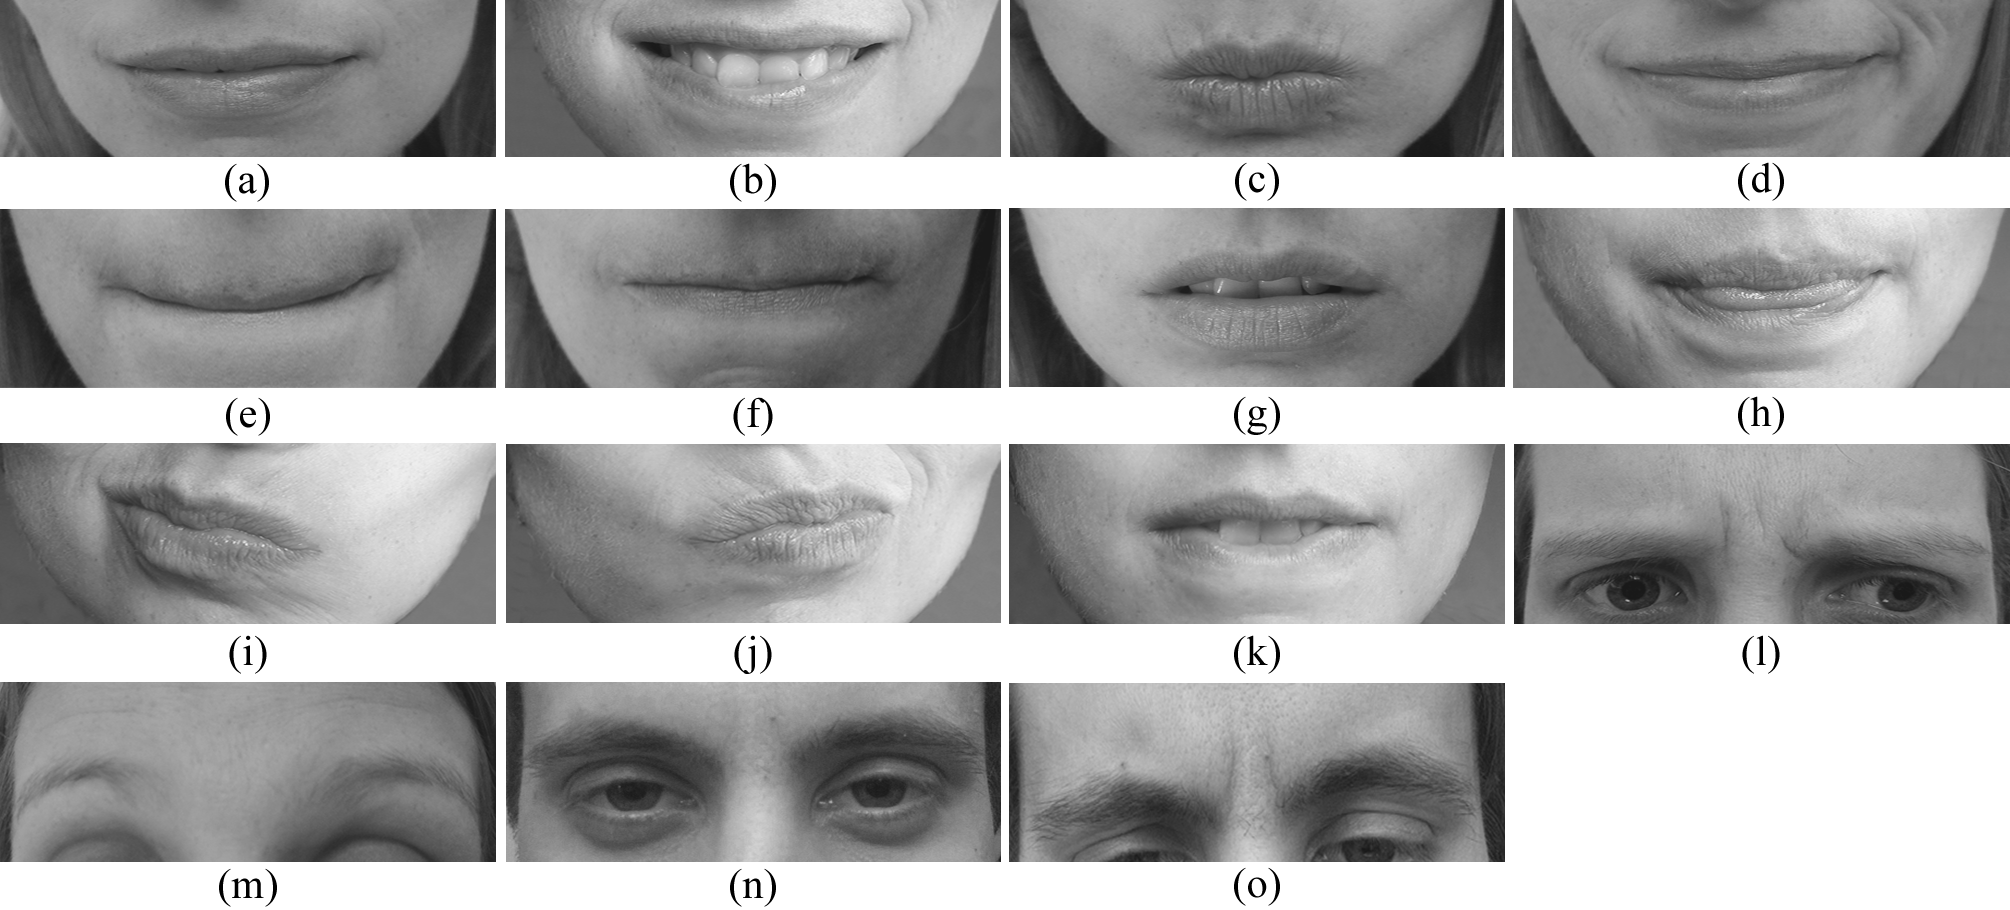
\includegraphics[width=0.4\textwidth]{figures/facial-actions}
\caption{Annotated facial actions (FA). (a) Smile not showing teeth; (b) Smile showing teeth; (c) Lip puckerer; (d) Lip stretcher; (e) Lip suck; (f) Lip pressor; (g) Lips parted; (h) Tongue touching lips; (i) Mouth movement right; (j) Mouth movement left; (k) Lower lip bite; (l) Frown; (m) Brow raiser; (n) Lid tightener; (o) Brow lowering}
\label{fig:fa}
\end{figure}

According to the design of the games, subjects are supposed to perceive the experience during the beginning of the games as being more boring than the one at the end, while the experience at the end should be perceived as more stressing than the one at the beginning of the games. As a result, if the game sessions of each subject is divided in half, in theory one of the two resulting parts is more likely to be perceived as more boring by the subjects, while the other is more likely to be perceived as more stressful. Using that assumption, FA annotations were divided in two groups, the ones made during the period that corresponds to the first half ($H_0$) of the games and the ones made in the second half ($H_1$). Such division of the annotation aimed to identify any pattern regarding FA happening during periods theoretically perceived as boring or stressful. After all annotations were made, an identification of uniqueness was performed and, based on that information, the repetitions of such unique actions across the games for all subjects was counted. As a result, the frequency that each FA appeared during all game sessions was obtained, as well as when they happened (in $H_0$ or $H_1$). Any FA that appeared just a single time during the whole 6 hours recording was excluded from the list, assuming that such action was noise or probably part of another action. As a result 17 unique FA that appeared in the recordings at least twice were identified. Excluding the talking and laughing FA, Figure \ref{fig:fa} illustrates all annotated FA. Finally after all annotations were counted and categorized according to the period in the game, a per-subject evaluation regarding the frequency of FA was conducted. For each subject, an inspection was performed regarding FA that appeared in $H_1$ of all three games with a higher frequency than in $H_0$, and vice versa (appeared in $H_0$ of all three games with a higher frequency than in $H_1$).

\subsection{Results}

\begin{table}[h!]
\caption{Amount of FA annotations made for all subjects during periods $H_0$ and $H_1$ of the games}
\label{table:amount-fa}
\centering
\begin{tabular}{L{.4\linewidth}C{.2\linewidth}C{.2\linewidth}}%
\toprule%
\textbf{Game} & \textbf{Period $H_0$} & \textbf{Period $H_1$} \\
\midrule
Mushroom   & 90 & 98 \\
\midrule
Platformer & 88 & 181 \\
\midrule
Tetris     & 110 & 159 \\
\bottomrule%
\end{tabular}%
\end{table}

The number of subjects that featured a particular FA was analized, alongside with the number of repetitions of such FA, for all three games. The analysis is also divided according to the period of the game. Only FA featured by two or more subjects were considered, since it produces an analysis that is connected to more frequent FA among the whole group of subjects instead of the peculiarities of a single person. Table \ref{table:amount-fa} shows the amount of FA annotations made for all subjects during the games. According to the results, the amount of FA annotations made during $H_1$ (second half) of all three games was greater than the amount of annotations made during $H_0$ (first half). The increase in annotations during $H_1$ compared to $H_0$ was 8.8\%, 105.6\% and 44.5\% higher for the Mushroom, Platformer and the Tetris game, respectively.

Regarding the FA annotated during each game, for the Mushroom game, the three most frequent FA in $H_0$ were frown (repeated 16 times among 5 subjects), talking (12 times, 3 subjects) and tongue touching lips (9 times, 3 subjects). The three most frequent FA in $H_1$ were frown (repeated 16 times among 3 subjects), talking (13 times, 5 subjects) and lips parted (13 times, 5 subjects). By comparing most frequent FA in the two periods, both frown and talking are present, however they were not featured by a significant number of participants. In fact no more than 5 subjects (25\% of the participants) featured one of those FA. It suggests that individuals present distinct facial behaviors that are not easily generalizable, even in the same context. Curiously, two particular FA presented a significant change in the amount of repetitions and subjects between the two periods: lip pressors (from 7 to 11 repetitions, 2 to 4 subjects) and lips parted (from 5 to 13 repetitions, 2 to 5 subjects). When compared to the whole group of participants, such increase is not significant (again they represent less than 25\% of the participants), but it might be the indication of a pattern for two or three subjects. As suggested by previous work, the combination of such particular changes with another physiological signal, e.g. HR, might produce an acceptable detector for boredom/stress emotional state.

For the Platformer game, the three most frequent FA for $H_0$ were frown (19 repetitions among 3 subjects), tongue touching lips (12 repetitions, 3 subjects) and smile not showing teeth (11 repetitions, 3 subjects). For $H_1$, the FA were frown (49 repetitions, 5 subjects), smile not showing teeth (21 repetitions, 7 subjects) and lips parted (17 repetitions, 5 subjects). By comparing the FA in both periods, frown was featured by more subjects (5, representing 25\%) during the stressful part of the game, however more participants (7, representing 35\%) also featured smiles not showing teeth as well. Additionally to those FA, 25\% of the participants featured talking behavior during $H_1$, externalizing game decisions.

For the Tetris game, the three most frequent FA for $H_0$ were frown (36 repetitions among 4 subjects), smile not showing teeth (14 repetitions, 4 subjects) and lip pressor (11 repetitions, 4 subjects). For $H_1$, the FA were frown (42 repetitions among 4 subjects), lip pressor (28 repetitions, 6 subjects) and smile not showing teeth (16 repetitions, 5 subjects). By comparing those results to the most frequent FA in the Mushroom game, only frown is present in both; it is important to stress that frown was featured by less than 25\% of the participants in both games, which highlights the difficulties in finding a pattern that can be applied to all subjects to identify a boring or a stressful situation, even when the most frequent FA are used. On the other hand, two FA presented a significant change from one period to another in the Tetris game: lip pressor (from 11 to 28 repetitions, 4 to 6 subjects) and talking (from 0 to 15 repetitions, 0 to 6 subjects). Both actions were featured by 30\% of the participants, which could be further investigated in the pursue of FA that can help in the identification of emotional states. Regarding the talking FA, it has been observed from the recordings that some subjects tended to externalize in words any wrong decisions they made in the game, such as how pieces were positioned, in a similar way observed during the Platformer game; in that sense, talking could be used as an indicator of activity in the game, since it is a clear facial manifestation that happened, in this case, when players were frustrated. For further FA analysis based on a group level, see \parencite{bevilacqua2016variations}.

Finally a per-subject inspection of all annotated FA was conducted according to the procedure described in Section \ref{s:experiment1-study1-methodology}. The aim was to identify, for each subjects, which FA appeared in $H_0$ (or $H_1$) of \emph{all} three games with a higher frequency than they did in $H_1$ (or $H_0$), if any. Table \ref{table:individual} shows the results of such inspection. Marked numbers represent the frequency of a FA that was present in all three games for the specified subject and period. In total 10 participants (50\%) featured at least one FA that appeared in all three games, in the same period (boring or stressful part) with a frequency equal or greater than its appearance in the counter-period. Subject 2, for instance, featured one lip pressor during $H_0$, while the total number of times the same FA appeared in $H_1$ for all three games combined was 18. It is important to highlight that subject 16 was the only one who featured a FA more frequently in $H_0$ of all three games than he/she did during $H_1$; all other subjects featured FA more frequently in $H_1$ than in $H_0$.

\begin{table}[!h]
\caption{Subject-based frequency of FA that appeared in the same period of all three games}
\label{table:individual}
\centering
\begin{threeparttable}
\begin{tabular}{cp{.4\linewidth}cc}
\toprule%
\textbf{Subject} & \textbf{FA} & \textbf{Period $H_0$} & \textbf{Period $H_1$} \\
\toprule%
2 & Lip pressor & 1 & 18\tnote{b} \\
\midrule
15 & Lip pressor & 2 & 9\tnote{b} \\
\midrule
10 & Laughing & 2 & 19\tnote{b} \\
\midrule
14 & Laughing & 3 & 9\tnote{b} \\
\midrule
12 & Smile not showing teeth & 2 & 8\tnote{b} \\
\midrule
13 & Smile not showing teeth & 0 & 6\tnote{b} \\
\midrule
18 & Smile not showing teeth & 4 & 10\tnote{b} \\
\midrule
11 & Lips parted & 1 & 10\tnote{b} \\
\midrule
17 & Lip stretcher & 0 & 8\tnote{b} \\
\midrule
16 & Talking & 7\tnote{b} & 1 \\
\bottomrule
\end{tabular}
\begin{tablenotes}
\small
\item[b]{FA was present in all three games for the specified subject and period.}
\end{tablenotes}
\end{threeparttable}
\end{table}

\subsection{Discussion}

About the FA, even though further investigation is required, calculations indicate that subjects featured a neutral face for a longer period of time during the first half ($H_0$) of all games when compared to the second half ($H_1$). Since FA annotations were made only when the subject's face featured anything different from her/his neutral face, more annotations indicate more facial activity. Additionally the results might indicate that subjects featured more FA (different from the neutral face) under stressful situations than they did under boring situations, where a neutral face/expression is probably dominant.

The games used in the experiment were designed to gradually increase the difficulty level until the subject was not able to handle it. As a consequence, it is possible to postulate that smiles and laughs during the second half could be connected to the subject's perception that the games were too difficult to continue playing properly. On the other hand, they could indicate genuine manifestations of enjoyment during the moments the subjects felt the game was properly balanced and engaging. Regarding the other FA, such as lip pressor and lips parted, further investigation is required to accurately connect or use such actions to predict/detect emotional states, however the results show a clue about how FA variations can be different on the individual level. As previously discussed, the analysis and generalization of FA on a group level is less clear than an individual approach, since FA behavior might be specific to each person. The per-subject analysis indicated that, for a portion of the participants, at least one FA was present in the three games, in the same period for the same person. Such information might be used as the starting point for further investigation regarding FA and an individual-tailored detection model for boredom/stress, for instance.

%%%%%%%%%%%%%%%%%%%%%%%%%%%%%%%%%%%%%%%%%%%%%%%%%%%%%%%%%%%%%%%%%%%%%%%%%%%%%%%%%%%%%
%\subsection{Limitations}
%%%%%%%%%%%%%%%%%%%%%%%%%%%%%%%%%%%%%%%%%%%%%%%%%%%%%%%%%%%%%%%%%%%%%%%%%%%%%%%%%%%%%

%One potential limitation of our work is the internal validity. As previously described, the experiment was based on a one-group posttest design, which does not use a control group to measure the effects of the treatment. Such design could be criticized for having low internal validity, since it is not possible to unambiguously attribute cause and effect \parencite{kirk1982experimental}. A two-group approach could be suggested as having stronger internal validity, since it contains a control group and allows a less ambiguous conclusion. In the context of our research, however, any multiple group design implies the comparison of physiological signals and emotional perceptions among different people. Given the social and cultural background of the participants, it is virtually impossible to compare two groups of people regarding stress/boredom. People have different preferences, culture and expectations, which cause maturation and history threats to internal validity \parencite{trochim2001research}. Additionally the process of comparing variations of physiological signals among different subjects is a complex task, even when subjects are similar, e.g. same age and sex. As a consequence, a subject in a control group might present a set of variations of signals and classify a game as boring, while a similar subject in another group might classify the same game as not boring at all, presenting a different set of variations of signals. In that light, our experiment relies on a one-group experimental design to increase internal validity, since subjects were compared with themselves, which removes inter-subject differences.

%Another limitation is the empirical approach used to annotate the FA, which was not based on a formal scheme and was conducted by a single person without validation by other researchers. We believe that the exploratory nature of our study regarding FA allows the use of such approach. Our aim was not to standardize FA regarding stress/boredom, but to document the perceptions of naked-eye observations of FA in a context involving games, so that it can be used to guide further steps regarding the utilization of FA in a multifactorial analysis. A frame-by-frame annotation of our video recordings using a formal scheme, such as FACS, would be a significantly laborious and time-consuming task, which is not motivated by our exploratory and empirical approach. Another limitation is the assumption used when dividing each game session in half, presuming that the middle point of the period indicates a transition from two distinct periods: $H_0$, perceived as more boring, and $H_1$, perceived as more stressing. It is not necessarily true. Even though our data indicate that subjects perceived the beginning of the games as being boring and the end as being stressful, our point of division or the periods themselves remain an assumption. There might be moments towards the end of the game, for instance, that could be perceived as more boring or joyful depending on the subject, since each participant has her/his own specific expectations and skill level regarding games. Finally the core mechanic of the Mushroom game is based on the color of the mushrooms (instead of patterns, for instance), which is not suitable for color blind subjects.

\subsection{Conclusion}

%This paper presented the description and results of an experiment aimed at exploring the variations of heart rate (HR) and facial actions (FA) during gaming sessions with induced boredom and stress. In total twenty adults of different ages and gaming experiences participated in the experiment, where they played three different games while being recorded by a video camera and monitored by a HR sensor. The games used in the experiment were carefully designed and implemented to have a difficulty level that linearly increases over time, from a boring to a stressful point. According to self-reported answers in post-games questionnaires, participants perceived the games as being boring at the beginning and stressful at the end. Such configuration gives our experiment a novel approach for the exploration of HR and FA regarding their connection to emotional states, since information can be categorized according to the induced (and theoretically known) emotional states.

Results show that more FA annotations were made during the stressful part of the games, which indicates that participants remained with a neutral face for longer periods of time during the boring part. The analysis on group level revealed that any FA pattern was related to 5 subjects (25\% of the group) at most. In the analysis conducted on the individual level, particular patterns were found for 10 subjects (50\% of the group).

%Our findings suggest that changes in the HR during gaming sessions is a promising indicator of stress, which could be incorporated into a model aimed at emotion detection. As pointed out by previous work, a user-tailored model based on several signals, e.g. HR and FA, is more likely to detect emotional states of users. In the context where the measurement of physiological signals by physical and contact-based sensors is intrusive or not desired, e.g. remote estimation of HR, information from different channels is required. One of such additional channels of information might be facial expressions, such as the FA analysis performed in this paper. For the context of our experiment, FA analysis on an individual level produced more information to connect FA and stress/boredom emotional states. We believe that this paper contributes with information regarding HR and FA in the context of games, which can be combined to create user-tailored models for emotion detection based on different data sources.

\section{Study 2: variations of heart rate}

\subsection{Introduction}

In order to explore the relation among facial actions, HR and emotional states, particularly stress and boredom, we designed and carried out an experiment involving games that were deliberately designed to cause the aforementioned emotional states. Our approach consists of recording participants while they play three different games that were carefully designed and developed to have a very similar difficulty balance that linearly progresses from a boring to a stressful state. Our experiment has two main goals. The first one is to measure the variations of the HR mean to test the hypothesis that the mean of the differences of HR during boring and stressful parts of the games is different. The second goal is to empirically explore how facial actions (FA), defined by us as being any facial movement different from a neutral face, e.g. lips contraction, manually detected and annotated with observations, relate to emotional states. Our experiment allows the investigation of variations of HR and FA in a context where boredom and stress were induced on purpose. As a result of our experiment, we present information regarding the changes in the HR mean of subjects while they play games that are deliberately boring and stressful; additionally we present a set of annotated FA that happened during the phases of the games that were perceived as being boring and stressful. Our main contribution is twofold: firstly we introduce information about the variations of HR that occurred during the interaction with the games, specially under situations that were designed to provoke boredom and stress. Our results indicate with statistical significance that the HR mean is different during boring and stressful situations in our games. Secondly we present information regarding the frequency which the annotations of naked-eye recognizable FA happened during specific phases of the games, all obtained from the analysis of about 6 hours of recordings from 20 subjects. We include an analysis and discussion of the gathered information. We believe that this paper contributes with information regarding HR and FA in the context of games, which can be combined to create user-tailored models for emotion detection based on different data sources. Additionally we highlight the heterogeneous nature of our group of subjects that have significantly different ages and gaming experiences, which produces a diverse sample for the investigation of changes in HR, FA and emotional states. In the remainder of this paper we will: summarize related works regarding the mapping of facial and physiological signals to emotional states; explain our experiment; show and discuss the results; finally we present a conclusion.

\subsection{Analysis and methods}

Firstly we removed from the set of all HR readings obtained during the experiment values that were equal to zero assuming they were miss-readings. After we calculated the baseline HR value for each subject ($B_s$) as:

\begin{equation} \label{eq:baseline}
B_s = \frac{1}{2}(\overline{HR}_{r1,s} + \overline{HR}_{r2,s})
\end{equation}

where $s$ indicates the subject and $\overline{HR}_{r1,s}$, $\overline{HR}_{r2,s}$ are the mean HR during the first and the second resting period (for subject $s$), respectively. $B_s$ is assumed to be the ``expected" HR of a given subject while resting. The average difference between $\overline{HR}_{r1,s}$ and $\overline{HR}_{r2,s}$ for each subject was 2.34 bpm.

We then calculated the HR mean coefficient $C_s^{g,t}$, which is the HR mean of a subject while playing a game during a given period of 60 seconds:

\begin{equation} \label{eq:variation}
C_s^{g,t} = \frac{1}{60}\sum_{n=1}^{60} HR_{s,g}(t\cdot 60 + n)
\end{equation}

where $s$ is the subject, $g$ is the game being played ($M$ for \underline{M}ushroom, $P$ for \underline{P}latformer or $T$ for \underline{T}etris), $t$ is the period and $HR_{s,g}(k)$ is the HR measured from subject $s$, in game $g$ at the mark of $k$ seconds. Since each subject played each game for more than 60 seconds, there is more than one period for each subject for a given game. The $t$ component of $C_s^{g,t}$ specifies which of such periods the HR mean refers to. For instance, $t=0$ comprehends the period from time 0:00 until time 1:00 of a given game, $t=1$ is the period from time 1:01 until 2:00, and so on. As an example, the HR mean coefficient $C_2^{P,1}$ is the HR mean of subject $2$ while playing the Platformer game from time 1:01 to 2:00.

HR values are specific to each individual, so we calculated the relativized HR mean coefficient, $V_s^{g,t}$, by subtracting $C_s^{g,t}$ from $B_s$ as:

\begin{equation} \label{eq:variation-normalized}
V_s^{g,t} = C_s^{g,t} - B_s
\end{equation}

$V_s^{g,t}$ accounts for values that are related to changes instead of absolute HR measurements, which are significantly more suitable for comparison among different subjects, or within the same subject.

Based on previous work regarding variations of HR and emotions, we state the following hypothesis: the HR mean during the last minute of gameplay is greater than the HR mean during the second minute of gameplay. More specifically, the true difference in means between $V^{g,n}$ (i.e. HR means when $t=n$, where $n$ is the last minute of gameplay) and $V^{g,1}$ (i.e. HR means when $t=1$, the second minute of gameplay) is greater than zero. The dependent variable is $V$ and the null hypothesis is that the true difference in means between $V^{g,n}$ and $V^{g,1}$ is less than or equal to zero. The reason why we choose $t=1$ (second minute of gameplay) instead of $t=0$ (first minute of gameplay) for our hypothesis is because we believe the first minute of the game might not be ideal for a fair comparison. Firstly during the first minute of gameplay, subjects are less likely to be in their usual neutral emotional state. They are more likely to be stimulated by the excitement of the initial contact with a game soon to be played, which interferes with any feelings of boredom. Secondly subjects need a basic understanding and experimentation with the game in order to judge if it is boring or not. As per our understanding, such conjecture is less likely to be fulfilled during the first minute of gameplay then it is to be during the second minute of gameplay.

\subsection{Results}

\begin{table*}[!t]
\renewcommand{\arraystretch}{1.0}
\caption{Values of $V_s^{g,t}$, the relativized HR mean coefficient, for all subjects ($s$) in a given game $g$ (M is for Mushroom, P for Platformer and T for Tetris), grouped by intervals ($t$) of 1 minute}
\label{table:hr}
\centering
\resizebox{\textwidth}{!}{
\begin{tabular}{|c|c|c|c|c|c|c|c|c|c|c|c|c|c|c|c|c|c|c|c|c|c|}
\hline
\multicolumn{2}{|c|}{} & \multicolumn{20}{|c|}{$s$} \\
\hline
$g$                   & $t$ & 1    & 2    & 3    & 4    & 5     & 6    & 7    & 8    & 9    & 10   & 11    & 12    & 13   & 14   & 15    & 16   & 17   & 18   & 19   & 20 \\
\hline
\multirow{7}{*}{M}    & 0   & -3.8 & 2.2  & -2.5 & -3.1 & -3.4  & -2.5 & 0.4  & 3.5  & -4.9 & -2.8 & -3.4  & -0.2  & -1.8 & 5.9  & -4.9  & 6.5  & -0.4 & -3.3 & 4.4  & 2.1  \\
                      & 1   & -9.1 & -1.4 & 0.3  & -2.6 & 0.2   & -3.7 & -1.5 & 2.7  & -4.9 & -4.1 & -10.3 & 0.0   & -3.1 & -3.1 & 0.2   & 5.6  & 2.5  & -0.8 & 0.5  & 3.2  \\
                      & 2   & -4.8 & -1.3 & -0.1 & -0.6 & 7.0   & 0.9  & 2.0  & 4.5  & -0.8 & -3.0 & -9.2  & 4.1   & 0.1  & -0.5 & -0.1  & 5.4  & 2.8  & 2.4  & 2.6  & 4.8  \\
                      & 3   & -4.9 & -0.7 & -2.8 & -1.5 & 1.5   & 0.3  & 2.4  & 5.1  & -2.4 & 1.7  & -4.6  & 2.4   & 0.4  & -0.2 & 0.7   & 4.5  & 3.4  & 3.8  & 2.4  & 3.5  \\
                      & 4   & -3.9 & -1.1 & 0.9  & 1.5  & 5.3   & 0.8  & 4.5  & 6.3  & 2.0  & 1.3  & -3.6  & 3.3   & 1.6  & 6.9  & 0.0   & 4.5  & 2.9  & 3.4  & 9.9  & 9.1  \\
                      & 5   & 0.3  & 2.4  & 1.4  & 1.7  & 11.9  & -1.2 & -    & -    & 4.4  & 10.2 & 1.6   & 6.2   & -    & -    & 3.2   & -    & 5.9  & 3.2  & 17.9 & 5.8 \\
                      & 6   & -    & -    & -1.2 & -0.1 & -     & -    & -    & -    & -    & -    & -     & -     & -    & -    & -     & -    & 3.3  & -    & -    & 6.7     \\
\hline
\multirow{5}{*}{P}    & 0   & -1.7 & 1.3  & 0.4  & -0.2 & 0.1   & 9.9  & 2.4  & -1.7 & -\textsuperscript{a}   & -1.9 & -2.7  & 0.8    & 5.7  & 19.7 & 6.0  & 0.2  & 5.9  & -1.2 & 4.2  & 5.5  \\
                      & 1   & -1.6 & -0.4 & 3.4  & -0.9 & -0.3  & 2.2  & 2.4  & 5.5  & -\textsuperscript{a}   & 2.4  & -4.4  & 0.7    & -1.5 & 4.1  & 4.9  & -1.0 & 0.8  & -0.2 & 3.7  & 7.7  \\
                      & 2   & 1.9  & 9.7  & 0.8  & -0.6 & 3.0   & -1.1 & 1.3  & 3.9  & -\textsuperscript{a}   & 15.1 & 0.2   & 3.5    & 3.9  & 3.8  & 11.7 & -0.7 & 2.8  & 0.4  & 4.0  & 10.6 \\
                      & 3   & 3.0  & 9.3  & 2.5  & -2.6 & 2.8   & 10.3 & 4.9  & 5.2  & -\textsuperscript{a}   & 21.6 & 3.2   & 5.4    & 9.2  & 4.6  & 9.9  & -    & 2.1  & 2.6  & 7.9  & 10.4 \\
                      & 4   & 5.9  & 6.8  & -    & 8.0  & 5.3   & -    & -    & -    & -\textsuperscript{a}   & -    & -     & -      & 4.9  & -    & 13.5 & -    & -    & -    & -    & -     \\
\hline
\multirow{6}{*}{T}    & 0   & 2.1  & 6.5  & -2.1 & -1.3 & -4.0  & 5.7  & 3.4  & 4.2  & 8.3  & 3.2  & 2.1   & -0.1  & 3.5  & 3.4  & 4.4  & -1.2 & 7.8  & -3.9 & 5.8  & 4.7  \\
                      & 1   & -2.7 & 0.0  & -3.3 & -1.2 & -4.9  & -0.1 & 4.3  & 4.2  & 2.7  & 2.9  & 0.0   & 2.6   & 2.2  & -2.5 & 5.9  & -1.3 & 4.2  & -0.4 & 5.7  & 0.0 \\
                      & 2   & -1.7 & 2.6  & 2.4  & -0.1 & -2.3  & 4.3  & 3.5  & -0.4 & 2.7  & 5.1  & 2.6   & 5.9   & 1.1  & -1.1 & 5.3  & -1.8 & 7.4  & 0.1  & 8.1  & 4.3  \\
                      & 3   & -1.9 & -0.2 & 0.3  & -2.2 & 0.8   & 5.4  & 2.1  & 3.8  & -    & 5.2  & 2.2   & 5.4   & -0.5 & -2.5 & 4.7  & -1.2 & 10.6 & 1.5  & 3.8  & 2.3  \\
                      & 4   & -0.8 & 3.0  & -    & 0.9  & -     & -    & -    & 7.8  & -    & 9.2  & 0.2   & 6.6   & -    & 3.4  & 5.6  & -1.2 & -    & 2.0  & 6.8  & 4.3  \\
                      & 5   & 1.5  & 7.4  & -    & -0.4 & -     & -    & -    & -    & -    & 12.9 & 7.4   & 4.5   & -    & 3.5  & 6.7  & -    & -    & -    & 6.9  & -    \\
\hline
\end{tabular}
}
\raggedright{\textsuperscript{a} Subject 9 had problems playing the Platformer game, so data from this subject during this game was excluded.}
\end{table*}

\begin{table}
    \caption{Mean of the differences of $V^{g,t}$ at the periods $t=1$ (second minute of gameplay) and $t=n$ (last minute of gameplay), for all subjects in each game ($g$). Values in bpm (beats per minute). Significance was tested with a one-tailed paired t-test}
    \label{table:proof}
    \centering
  \begin{threeparttable}
     \begin{tabular}{|c|>{\centering\arraybackslash}p{5.2cm}|}
        \hline
        \textbf{Game ($g$)} & \textbf{Mean of the differences between\newline $V^{g,n}$ and $V^{g,1}$} \\
        \hline
        Mushroom (M) & 6.11 ***  \\
        \hline
        Platformer (P) & 5.10 ***  \\
        \hline
        Tetris (T) & 3.33 *** \\
        \hline
     \end{tabular}
    \begin{tablenotes}
      \small
      \item[***]{$p < 0.001$}
    \end{tablenotes}
  \end{threeparttable}
\end{table}


\begin{table}[!t]
\renewcommand{\arraystretch}{1.2}
\caption{Mean of the differences of $V^{g,t}$ at key periods, for all subjects in a given game $g$ (M is for Mushroom, P for Platformer and T for Tetris). Values in bpm (beats per minute)}
\label{table:mean}
\centering
\begin{tabular}{|>{\centering\arraybackslash}p{0.5cm}|>{\centering\arraybackslash}p{1.3cm}|>{\centering\arraybackslash}p{1.3cm}|>{\centering\arraybackslash}p{1.3cm}|>{\centering\arraybackslash}p{1.3cm}|}
\cline{2-5}
\multicolumn{1}{c|}{} & \multicolumn{4}{|c|}{\textbf{Pairs}} \\
\hline
\textbf{$g$} & \textbf{$V^{g,1}$,\newline$V^{g,0}$} & \textbf{$V^{g,n}$,\newline$V^{g,n-1}$} & \textbf{$V^{g,n}$,\newline$V^{g,0}$} & \textbf{$V^{g,n-1}$,\newline$V^{g,1}$} \\
\hline
M & -0.87   & 2.39 & 5.23 & 3.71 \\
\hline
P & -1.31   & 2.57 & 3.78  & 2.52  \\
\hline
T & -1.71 & 1.22  & 1.62    & 2.10 \\
\hline
\end{tabular}
\end{table}

Table \ref{table:hr} presents the values of $V$, the relativized HR mean coefficient, for all subjects in all games, grouped by intervals of 1 minute, calculated according to the description in Section \ref{s:methodology}. Column $g$ is the game being played, $t$ is the period in the game and $s$ is the subject. Since all games were constantly changing in difficulty and subjects have different gaming skills, there are subjects with no data entry for some $t$ intervals, which means he/she was defeated by the game earlier than other subjects were. Subject 9 had problems playing the Platformer game, so data for that subject in that game was not used in the calculations.

A positive value in Table \ref{table:hr} represents a $V$ (HR mean) that is above the subject's baseline $B_s$ (mean HR while resting) for an specific period $t$. A negative value indicates that $V$ in that period is below the subject's baseline $B_s$. Assuming $n$ as the last minute of gameplay of a given subject in a game, by comparing the values at $t=0$ (first minute of the gameplay, perceived as boring) and $t=n$ (last minute of gameplay, perceived as stressful) in the Mushroom game, 19 subjects (95\%) presented $V^{M,n}$ greater than $V^{M,0}$. The same comparison regarding the Platformer game indicates that 16 subjects (84.2\%) had higher $V^{P,n}$ than $V^{P,0}$. In the Tetris game 13 subjects (65\%) presented higher $V^{T,n}$ than $V^{T,0}$.

As previously mentioned, our null hypothesis is that the true difference in means between $V$ at the last minute of gameplay ($t=n$) and at the second minute of gameplay ($t=1$) is less than or equal to zero. Table \ref{table:proof} shows the mean of the differences of a one-tailed paired t-test on the values of $V^{g,n}$, i.e. last minute of gameplay for a given game $g$, and $V^{g,1}$, i.e. second minute of gameplay for a given game $g$, for all games and subjects. Results indicate the difference is greater than zero with statistical significance for all games. For the Mushroom game, the mean of the differences between the last ($V^{M,n}$) and the second ($V^{M,1}$) minutes of gameplay is $6.11$ bpm ($p < 0.001$). For the Platformer game, the mean of the differences of $V^{P,n}$ and $V^{P,1}$ is $5.1$ bpm ($p < 0.001$). Finally, for the Tetris game, the mean of the differences of $V^{T,n}$ and $V^{T,1}$ is $3.33$ bpm ($p < 0.001$). Those numbers reject the null hypothesis, thus supporting our experimental hypothesis that the HR mean during the last minute of gameplay is greater than the HR mean during the second minute of gameplay, for all games.

In order to further explore the mean variation of HR at key periods other than the ones in our hypothesis, we calculated the mean of the differences involving $V^{g,0}$, $V^{g,1}$, $V^{g,n}$ and $V^{g,n-1}$, for all games and subjects. Results are shown in Table \ref{table:mean}. $V^{g,0}$ and $V^{g,1}$ are the values of $V$ for a given game $g$ during the first and the second minute of gameplay, respectively. $V^{g,n}$ and $V^{g,n-1}$ represent the values of $V$ for a given game $g$ during the last and the immediately before the last minute of gameplay, respectively. As previously mentioned, the value of $n$, the last minute of gameplay, is different for each subject since subjects might have been defeated by the game at different moments due to personal skill levels.

In the first two minutes of gameplay ($t=0$ and $t=1$), the mean of the differences between $V^{g,1}$ and $V^{g,0}$ is negative for all games. The mean of the differences is $-0.87$ bpm for the Mushroom game ($V^{M,1}$ and $V^{M,0}$), $-1.31$ bpm for the Platformer game ($V^{P,1}$ and $V^{P,0}$) and $-1.71$ bpm for the Tetris game ($V^{T,1}$ and $V^{T,0}$). Those numbers suggest a higher HR mean during the first minute of the games ($t=0$) than during the second minute ($t=1$). At the last two minutes of gameplay ($t=n$ and $t=n-1$), the mean of the differences between $V^{g,n}$ and $V^{g,n-1}$ is positive for all games. The mean of the differences is $2.39$ bpm for the Mushroom game ($V^{M,n}$ and $V^{M,n-1}$), $2.57$ bpm for the Platformer game ($V^{P,n}$ and $V^{P,n-1}$) and $1.22$ bpm for the Tetris game ($V^{T,n}$ and $V^{T,n-1}$). Those numbers suggest a higher HR mean during the last minute of the game ($t=n$) compared to the penultimate minute ($t=n-1$).

Regarding the last ($t=n$) and the first ($t=0$) minutes of gameplay, the mean of the differences between $V^{g,n}$ and $V^{g,0}$ is $5.23$ bpm for the Mushroom game ($V^{M,n}$ and $V^{M,0}$), $3.78$ bpm for the Platformer game ($V^{P,n}$ and $V^{P,0}$) and $1.62$ bpm for the Tetris game ($V^{T,n}$ and $V^{T,0}$). Regarding the penultimate ($t=n-1$) and the second ($t=1$) minutes of gameplay, results show that the mean of the differences between $V^{g,n-1}$ and $V^{g,1}$ is $3.71$ bpm for the Mushroom game ($V^{M,n-1}$ and $V^{M,1}$), $2.52$ bpm for the Platformer game ($V^{P,n-1}$ and $V^{P,1}$) and $2.1$ bpm for the Tetris game ($V^{T,n-1}$ and $V^{T,1}$). Both sets of numbers suggest a higher HR mean during the last minute of the game ($t=n$) compared to the first minute ($t=0$), as well as a higher HR mean during the penultimate minute of gameplay ($t=n-1$) compared to the second minute ($t=1$).

\subsection{Discussion}

A number of subjects presented a higher value for $V$, the relativized HR mean coefficient, towards the end of the Mushroom and the Platformer games when compared to the same period of the Tetris game, as shown by Table \ref{table:hr}. Both the Mushroom and the Platformer game were completely new to the subjects, since they were developed exclusively for the experiment. For the self-reported 5-point Likert scale regarding familiarity with the games/genres, the mean value was 2.75 for the Mushroom, 2.8 for the Platformer and 3.35 for the Tetris game (5 being extremely familiar). Such numbers could indicate that subjects were less likely to predict what was going to happen in the Mushroom and the Platformer when compared to the Tetris game. It could explain the greater number of subjects with higher $V$ during the end (stressful) part of those two games when compared to the smaller number of subjects with higher $V$ at the end of Tetris. The later is a popular game and subjects were more familiarized with it, so they might be more likely to guess what is about to happen in the game, reducing anxiety levels. This is specially true if the subject is trained to deal with the inherent stress of the mechanic, for instance.

A significant number of subjects presented a negative value for $V$ in some periods. In total 16 subjects (80\%) in the Mushroom game, 11 (57.8\%) in the Platformer and 12 (60\%) in the Tetris game presented negative values. A negative value indicates that the subjects had a lower HR mean while playing the game at specific periods than while resting. After the experiment, some subjects reported discomfort during the resting period, mentioning that it was too long and boring. We believe the resting period might have been stressful for some subjects, as they were required to rest while being seated without any entertainment, e.g. mobile phones. Another explanation for such negative values is that our calculation of the subject's baseline $B_s$ might be a weak approximation of the real HR mean of each subject during rest, since we only measured two 140-seconds long resting situations for each subject. We believe, however, that our baseline calculation is still a good parameter, since the average difference between the mean HR of the two resting periods was significantly low, as explained in Section \ref{s:methodology}.

Regarding the confirmation of our hypothesis, the mean of the differences between $V$ at the last ($t=n$) and the second ($t=1)$ minutes of gameplay, presented in Table \ref{table:proof}, shows statistical significance in the difference for all games. It reinforces findings of previously mentioned works \parencite{vandeput2009heart, garde2002effects, bousefsaf2013remote, rodriguez2015vr, yamakoshi2007preliminary} which indicate that HR tends to be higher (above the subject's baseline) during stressful moments and lower (closer to subject's baseline) during boring moments in a gaming context. As previously described, the reason why we used $t=1$ (second minute of gameplay) instead of $t=0$ (first minute of gameplay) for our main comparison is because we believe the first minute of all games might not be ideal for a fair comparison. During the first minute, subject are less likely to be in their usual neutral emotional state. Such line of reasoning is supported by the exploratory analysis of the mean of the differences of $V$ at periods other than the ones used in our hypothesis, as presented in Table \ref{table:mean}. In the beginning of the games, the HR mean during $t=0$ (0:00 to 1:00) was higher than during $t=1$ (1:01 to 2:00) for all three games. It could indicate that subjects were more stimulated at the very beginning, probably caused by the excitement of the initial contact with a game to be played. We believe that such difference during $t=1$ and $t=0$ could also be explained as a response to the fact that subjects probably understood the game mechanic. During the first minute of gameplay, subject are probably still working to understand the game, so an opinion regarding boredom is still being formed. After the one minute mark, subject are more likely to have fully understood the game, so they could judge it was boring. Additionally, a better understanding of the mechanic combined with the fact that subjects were not allowed to change the game pace, e.g. to make it more interesting, probably increased the feeling of boredom.

%%%%%%%%%%%%%%%%%%%%%%%%%%%%%%%%%%%%%%%%%%%%%%%%%%%%%%%%%%%%%%%%%%%%%%%%%%%%%%%%%%%%%
\subsection{Limitations}
%%%%%%%%%%%%%%%%%%%%%%%%%%%%%%%%%%%%%%%%%%%%%%%%%%%%%%%%%%%%%%%%%%%%%%%%%%%%%%%%%%%%%

One potential limitation of our work is the internal validity. As previously described, the experiment was based on a one-group posttest design, which does not use a control group to measure the effects of the treatment. Such design could be criticized for having low internal validity, since it is not possible to unambiguously attribute cause and effect \parencite{kirk1982experimental}. A two-group approach could be suggested as having stronger internal validity, since it contains a control group and allows a less ambiguous conclusion. In the context of our research, however, any multiple group design implies the comparison of physiological signals and emotional perceptions among different people. Given the social and cultural background of the participants, it is virtually impossible to compare two groups of people regarding stress/boredom. People have different preferences, culture and expectations, which cause maturation and history threats to internal validity \parencite{trochim2001research}. Additionally the process of comparing variations of physiological signals among different subjects is a complex task, even when subjects are similar, e.g. same age and sex. As a consequence, a subject in a control group might present a set of variations of signals and classify a game as boring, while a similar subject in another group might classify the same game as not boring at all, presenting a different set of variations of signals. In that light, our experiment relies on a one-group experimental design to increase internal validity, since subjects were compared with themselves, which removes inter-subject differences.

\subsection{Conclusions}

This paper presented the description and results of an experiment aimed at exploring the variations of heart rate (HR) and facial actions (FA) during gaming sessions with induced boredom and stress. In total twenty adults of different ages and gaming experiences participated in the experiment, where they played three different games while being recorded by a video camera and monitored by a HR sensor. The games used in the experiment were carefully designed and implemented to have a difficulty level that linearly increases over time, from a boring to a stressful point. According to self-reported answers in post-games questionnaires, participants perceived the games as being boring at the beginning and stressful at the end. Such configuration gives our experiment a novel approach for the exploration of HR and FA regarding their connection to emotional states, since information can be categorized according to the induced (and theoretically known) emotional states.

The HR data related to the game session of each subject was divided in periods of 1 minute each, whose HR mean was calculated and compared to a baseline value obtained from the HR mean of the subject during rest. Based on the self-reported answers regarding stress and boredom, we analysed the HR mean at specific periods, such as the second minute of gameplay (perceived as boring) and the last minute of gameplay (perceived as stressful). Our results indicate that the average HR mean for all subjects during the last minute of gameplay was greater than the average HR mean during the second minute of gameplay, for all games with statistical significance ($p<0.001$). Our findings are aligned with and reinforce previous research that indicate higher HR mean during stressful situations in a gaming context. The design of our games permitted a more elaborated analysis of boring and stressful periods, which contributes information regarding variations of HR mean during such conditions in gaming sessions. Additionally we performed an exploratory investigation regarding HR mean during other key periods in the games, e.g. first and penultimate minutes of gameplay. Further analysis is still required, however our numbers suggest that the average HR mean during the first minute of gameplay was greater than during the second minute of gameplay, probably as a consequence of unusual excitement during the first minute, e.g. the idea of playing a new game.

Our findings suggest that changes in the HR during gaming sessions is a promising indicator of stress, which could be incorporated into a model aimed at emotion detection. As pointed out by previous work, a user-tailored model based on several signals, e.g. HR and FA, is more likely to detect emotional states of users. In the context where the measurement of physiological signals by physical and contact-based sensors is intrusive or not desired, e.g. remote estimation of HR, information from different channels is required. One of such additional channels of information might be facial expressions, such as the FA analysis performed in this paper. For the context of our experiment, FA analysis on an individual level produced more information to connect FA and stress/boredom emotional states. We believe that this paper contributes with information regarding HR and FA in the context of games, which can be combined to create user-tailored models for emotion detection based on different data sources.

\section{Study 3: heart rate and accuracy of rPPG measurements}
\label{s:study3}

This study presents information regarding the accuracy evaluation of a remote photoplethysmography (rPPG) technique in a gaming context. The technique was applied to estimate the HR of subjects behaving naturally in gaming sessions with induced boredom and stress. Previous work with experiments involving emotions and rPPG were performed under extremely controlled situations with few game-related stimuli. Subjects were not interacting with a complete digital game in any of the experiments, which hindered the accuracy evaluation of rPPG techniques within the context of games research, for instance. Authors commonly used images, videos or text as content to produce the emotional stimuli, in experimental sessions lasting from 20 seconds to 10 minutes.

The aforementioned non-game stimuli content is less likely to produce the reactions of a real gaming session, e.g. spontaneous body movement and facial actions. As opposed to such works, in this study each subject spent an average of 25 minutes in the session, playing three different games that were custom-made to provoke the emotional reactions similar to a natural play session. Subjects were also not instructed regarding how they should move, so body and facial reactions are likely to be the ones the subject would normally perform under a gaming context.

The recordings of game sessions of each subject were divided in video segments of 1 minute each. The rPPG technique by Poh et al. \parencite{poh2011advancements} was applied to each of those video segments to estimate the HR of subjects. An accuracy evaluation of the estimated HR obtained from the video segments was performed in relation to the HR calculated from ground truth.

%however its reliability within a context involving natural behavior must be checked. The methods are sensitive to noise caused by movement, facial expressions or changes in illumination (e.g. screen activity reflected on user's face), which are all likely to happen in such sessions with natural behavior. Those interferences might produce unreliable measurements of the HR signal, resulting in misleading investigations. It is important to establish the reliability of remote HR measurements under situations with natural behavior, where users are not instructed to behave differently than what they usually do. In that light this paper presents an analysis of the remotely obtained HR signal of users within such natural context. We developed a set of casual-themed, similar to off-the-shelf games that were carefully designed to present stressful and boring moments, which should induce players to present variations of HR. During the gaming sessions, the player's HR signal was remotely estimated using the work by \textcite{poh2011advancements}, an established rPPG technique for HR estimation. A physical sensor was used as ground truth. A comparison and analysis of the accuracy of remote HR estimations are presented and discussed. The main contribution of this paper is the accuracy evaluation of an established rPPG technique within the context of gaming sessions where users behave naturally instead of following movement constraint rules, e.g. remain still. Our results provide researchers with information related to the reliability of a remote HR measurement technique when applied to contexts where users behave more naturally

%The use of remote measurement of physiological signals, such as rPPG, has already been applied to emotion detection. Signals as HR and HRV were used to remotely detect stress \parencite{mcduffcogcam, mcduff2014improvements, bousefsaf2013remote}, for instance. Since the estimations of rPPG techniques are significantly affected by external noise, e.g. subject's movement, experimental results are usually accompanied by accuracy evaluations regarding the estimations of the employed rPPG technique. In the majority of the cases, subjects are typically instructed to stay still \parencite{rouast2016remote}, which improves the accuracy of the rPPG technique. In some other cases, however, authors evaluate the accuracy of the HR estimation under scenarios where subjects are instructed to act naturally. Despite the fact that such works present experiments where subjects are told to behave naturally, their accuracy evaluation is based on artificial or simple human-computer interactions. Subjects are idly staring at the camera \parencite{zhao2013remote,hsu2014learning}, faking an interaction with a computer \parencite{poh2010non}, working on a task, i.e. make a website \parencite{monkaresi2014machine} or mentally subtract numbers \parencite{mcduff2014remote}, or performing arbitrary movements \parencite{tran2015robust}, e.g. head rotation in different degrees.

%Another important factor is the material used to produce the emotional stimuli. Subjects are not interacting with a complete digital game in any of the experiments, which hinders the accuracy evaluation of rPPG techniques within the context of games research, for instance. Authors commonly use images, videos or text as content to produce the emotional stimuli. When game-like materials are used, however, they are often gamified cognitive tests, e.g. Stroop test \parencite{golden1978stroop}. Additionally the experiment duration varies from 20 seconds to 10 minutes and the non-game stimuli content is less likely to produce the reactions of a real gaming session, for instance spontaneous body movement and facial actions.

%In that context, we designed and carried out an experiment focused on the accuracy evaluation of an rPPG technique applied to real gaming sessions, using custom made games as emotion stimuli.  We aim to explore the accuracy of rPPG-estimated HR readings of subjects while playing under such circumstances. To the best of our knowledge, this is the first experiment to measure the accuracy of an rPPG technique with the use of three boredom/stress-inducing games with subjects behaving naturally.

\subsection{Analysis and methods}

Firstly the videos of each game session were divided into several video segments of 60 seconds each, denoted as $V_i$, where $i \in [1, 2, ..., n]$ represents the interval (1 comprehends the time from 0:00 until 1:00, 2 comprehends the time from 1:00 until 2:00, and so on). The use of 60 seconds as the duration of each video segment is based on the work by \textcite{poh2011advancements}.

Since the games have a constantly increasing difficulty level, different subjects might have played the same game for longer or shorter periods of time. As a consequence, the interval $n$ represents the last available interval for each subject and it is likely to be different among subjects. Any remaining video segment of less than 60 seconds was discarded, i.e. if the duration of a game session was not multiple of 60. Following was the calculation of $HR_{gt}(V_i)$, which is the mean HR obtained from the ground truth data of a subject while playing during the video segment $V_i$. It was excluded from the calculation any HR value equal to zero assuming it was a miss-reading.

As previously mentioned in Section \ref{s:literature-rppg-techniques}, the rPPG technique proposed by \textcite{poh2011advancements} is consolidated, extensively mentioned in the literature and presents the best SNR for HR estimation under non-exercising situations. For those reasons, such technique  (refereed as the rPPG technique from now on) was selected to perform the extraction of HR from the video segments. For the comparison, $HR_{video}(V_i)$ was calculated, which is the estimated HR from video segment $V_i$ obtained with the rPPG technique. The evaluation of the accuracy of $HR_{video}$ when compared to $HR_{gt}$ was based on statistical methods used by previous works \parencite{poh2011advancements, rouast2016remote, li2014remote}. The measurement error is calculated as:

\begin{equation}
\label{eqn:hr-error}
HR_{error} = HR_{video} - HR_{gt}
\end{equation}

where $HR_{video}$ is the set of HR estimations by the rPPG technique from the video segments and $HR_{gr}$ is the set of HR means calculated from the ground truth obtained from the watch, as previously described in Section \ref{s:study3}. $HR_{error}$ was calculated with video segments of a given game (for the analysis of that game) or with all available segments (for the analysis of all games combined).

The following measurements were also calculated: mean of $HR_{error}$ denoted as $M_e$; standard deviation of $HR_{error}$ denoted as $SD_e$; root mean squared error (RMSE) of $HR_{error}$; mean of error-rate percentage, calculated as:

\begin{equation}
\label{eqn:merate}
M_{eRate} = \frac{1}{N} \sum_{i=1}^{N}\frac{|HR_{error}(V_i)|}{HR_{gt}(V_i)}
\end{equation}

where $V_i$ is a video segment and $N$ is the total of video segments for a given game (or for all games); finally the linear correlation between $HR_{video}$ and $HR_{gt}$ accessed using Pearson's correlation coefficient $r$.

%%%%%%%

The selected rPPG technique was implemented in Matlab R2016a according to the original paper by \textcite{poh2011advancements}. Since the custom algorithm to detect peaks mentioned in the article is unknown, such step was replaced by the identification of the highest peak in the frequency domain after an FFT operation. This operation is commonly used in the HR estimation phase of rPPG techniques, as explained in Section \ref{s:literature-rppg-structure}.

The implementation of the rPPG technique was validated with a procedure similar to the one described by \textcite{li2014remote}. Firstly a manual inspection of all video recordings from the experiment was performed and a segment $V'_i$ of 30 seconds (1500 frames) was exerted from each video where the subject presented the least amount of body motion and facial activity. It resulted in a testing set of 20 video segments of 30 seconds each, totalizing 30000 frames of data. The mean HR calculated from ground truth for the testing set was 76.8 bpm (SD 13.4 bpm, min. 55 bpm, max. 110 bpm).

The rPPG technique was then applied to each of those $V'_i$ segments to estimate the HR, evaluating the estimated values using ground truth and the statistical methods previously described. Results are presented in Table \ref{table:rppg-validation}. The numbers indicate the implemented rPGG technique produces accurate and statistically significant results for the estimations, which are aligned with those reported in the original paper. Therefore it is assumed the rPPG technique is correctly implemented and further accuracy measurements obtained during the analysis are due to subject activity, not implementation errors.

\begin{table}
\caption{Performance of the rPPG technique applied to the testing set}
\label{table:rppg-validation}
\centering
\begin{threeparttable}
  \begin{tabular}{ccccc}
  \toprule
    $M_e$ (bpm) & $SD_e$ (bpm) & RMSE (bpm) & $M_{eRate}$ (\%) & $r$ \\
  \midrule
    -0.25 & 1.41 & 1.40 & 1.52 & 0.99* \\
  \bottomrule
  \end{tabular}
  \begin{tablenotes}
    \small
    \item[*]{$p < 0.001$}
  \end{tablenotes}
\end{threeparttable}
\end{table}

\subsection{Results}

The performance of the rPPG technique regarding the extraction of the HR is presented on Table \ref{table:rppg-validation-games}. The first three rows of the table present the performance evaluation calculated with data from each game, while the last row presents the same performance evaluation calculated with data from all games combined. Regarding the analysis of all games combined, the mean estimation error $M_e$ was 2.99 bpm ($SD_e$ 18.83 bpm), RMSE was 19.03 bpm and $M_{eRate}$ was 10.31\%. The low value for $M_e$ suggests feasible overall accuracy of the technique, however the high values for $SD_e$ and $M_{eRate}$ suggest significant variation among the estimations.

As demonstrated by $M_{eRate}$, which is the mean of error-rate percentage, the estimation error of the rPPG technique was equivalent to 10.31\% of the expected HR value calculated from ground truth, on average. On a game level, the mean estimation error $M_e$ was 2.96 bpm ($SD_e$ 19.45 bpm) in the Mushroom game, 0.31 bpm (13.51 bpm) in the Platformer game and 5.18 bpm (21.45 bpm) in the Tetris game. RMSE and $M_{eRate}$ were 19.59 bpm and 10.88\% in the Mushroom game, 13.43 bpm and 7.82\% in the Platformer game, and 21.97 bpm and 11.64\% in the Tetris game, respectively.

All three games presented acceptable values for $M_e$ and significantly higher values for $SD_e$ and $M_{eRate}$, which also suggests feasible results with considerable variations in the estimation error during the analysis of subjects for each game. In particular, the estimations performed during the Platformer game presented the lowest values for $M_e$, RMSE and $M_{eRate}$, which indicates the rPPG technique performed with lower errors and fewer variations among subjects in the Platformer game than it did in the other two games.

\begin{table}
\caption{Accuracy measurements of the rPPG technique when applied to the video segments of a given game and of all games}
\label{table:rppg-validation-games}
\begin{threeparttable}
  \begin{tabular}{p{0.13\linewidth}ccccp{0.04\linewidth}}%
  \toprule
     Game & $M_e$ (bpm) & $SD_e$ (bpm) & RMSE (bpm) & $M_{eRate}$ (\%) & $r$ \\
  \midrule
      Mushroom & 2.96 & 19.45 & 19.59 & 10.88 & 0.45* \\
      Platformer & 0.31 & 13.51 & 13.43 & 7.82 & 0.55* \\
      Tetris & 5.18 & 21.45 & 21.97 & 11.64 & 0.37* \\
      \textit{All} & 2.99 & 18.83 & 19.03 & 10.31 & 0.43* \\
  \bottomrule
  \end{tabular}
  \begin{tablenotes}
    \small
    \item[*]{$p < 0.001$}
  \end{tablenotes}
\end{threeparttable}
\end{table}

The Pearson's correlation coefficient $r$ regarding $HR_{gt}$ (mean HR calculated from the ground truth) and $HR_{video}$ (mean HR estimated via rPPG) is 0.45, 0.55 and 0.37 for the Mushroom, Platformer and Tetris game, respectively. All correlations have statistical significance, $p < 0.001$. The correlation is illustrated in Figure \ref{fig:chart-r-games}. For all three games, there is a positive and medium strength correlation between $HR_{gt}$ and $HR_{video}$, which also indicates the estimations performed by the rPPG technique are feasible. The correlation is stronger in the Platformer game, followed by the Mushroom game and finally by the Tetris game.

\begin{figure}[!h]
\centering
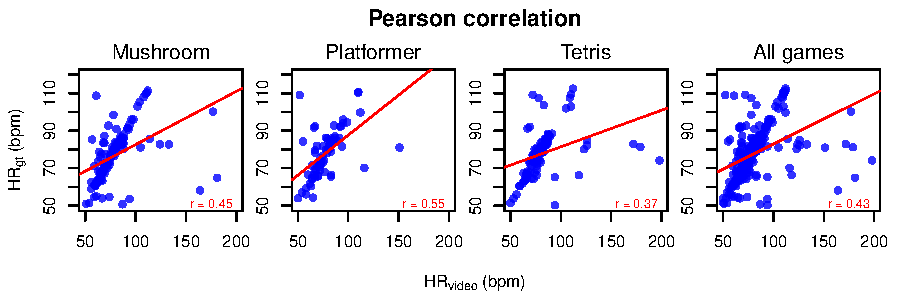
\includegraphics[width=\columnwidth]{figures/correlation-hrgt-hrvideo.pdf}
\caption{Statistical correlation of $HR_{gt}$ and $HR_{video}$ when applied to the video segments of each game, as well as to the video segments of all games.}
\label{fig:chart-r-games}
\end{figure}

To better analyze the variations regarding estimation errors among subjects, figures \ref{fig:chart-hists-me} and \ref{fig:chart-hists} show a distribution of values of $M_e$, RMSE and $M_{eRate}$ for all games combined and individually. The x-axis represents intervals of values of $M_e$, RMSE or $M_{eRate}$ while the y-axis represents the percentage of subjects that presented an estimation error within the interval informed in the x-axis.

Regarding the distribution of values of $M_e$, shown in Figure \ref{fig:chart-hists-me}, overall 66.1\% of the subjects presented estimations with $M_e$ within the interval [-5 bpm, 5 bpm]. For the remaining 33.9\% of the subjects, $M_e$ was spread within the interval [-20 bpm, 35 bpm]. On a game level, $M_e$ was within the interval [-5 bpm, 5 bpm] for 65\%, 68.4\% and 65\% of the subjects of the Mushroom, Platformer and Tetris game, respectively. The values for $M_e$ are more equally distributed for the Platformer game, which explains the lower values of $SD_e$ for that game when compared to the Mushroom and the Tetris game, which present less equally distributed values of $M_e$.

The distribution of values of RMSE, shown in Figure \ref{fig:chart-hists} in the first row, indicate that overall values were lower then 10 bpm for 59.4\% of the subjects, while the remaining of the subjects had RMSE varying from 10 bpm to 50 bpm. On a game level, RMSE was lower than 10 bpm for 50\%, 68.5\% and 60\% of the subjects of the Mushroom, Platformer and Tetris game, respectively.

Regarding $M_{eRate}$, shown in Figure \ref{fig:chart-hists} in the second row, overall 69.5\% of subjects had HR estimations that were up to 10\% different than the expected HR from ground truth. On a game level, in total 73.7\% and 70\% of the estimations performed by the rPPG technique during the Platformer and the Tetris game, respectively, presented $M_{eRate}$ interior or equal to 10\%. Those values are slightly better than the 65\% of the subjects with $M_{eRate}$ up to 10\% in the Mushroom game. Despite the fact that $M_{eRate}$ was similar for both the Platformer and Tetris games, the former presented no subjects whose $M_{eRate}$ was greater than 30\%, while the later presented 10\% of the subjects with $M_{eRate}$ greater than 30\%.

\begin{figure}[!h]
\centering
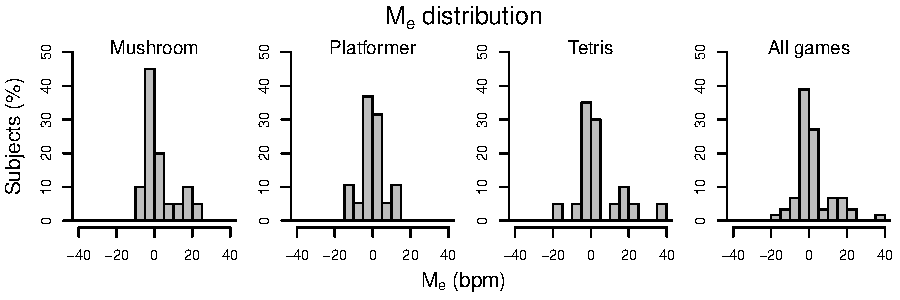
\includegraphics[width=1.0\textwidth]{figures/hist-me.pdf}
\caption{Distribution of values of $M_e$ for all games. The x-axis represents intervals of values of $M_e$ while the y-axis represents the percentage of subjects that presented an estimation error within the interval informed in the x-axis.}
\label{fig:chart-hists-me}
\end{figure}

\begin{figure}[!h]
\centering
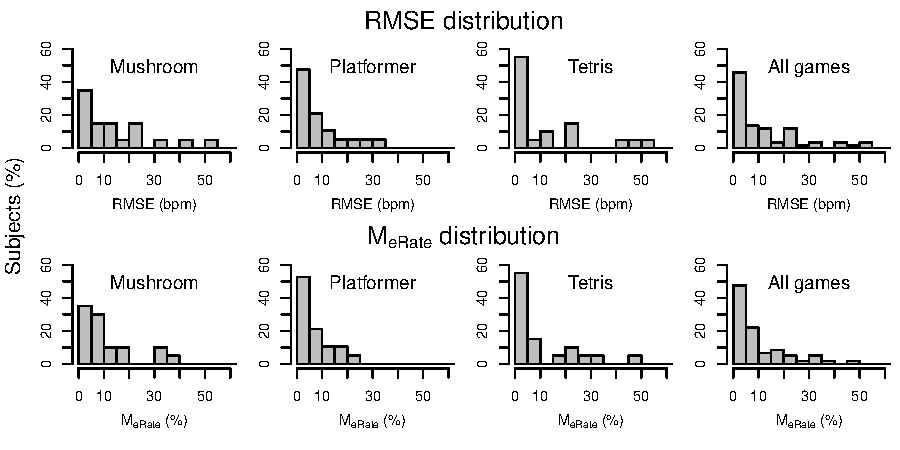
\includegraphics[width=1.0\textwidth]{figures/hist-rmse-mrate.pdf}
\caption{Distribution of values of RMSE and $M_{eRate}$ for all games. The x-axis represents intervals of values of RMSE or $M_{eRate}$ while the y-axis represents the percentage of subjects that presented an estimation error within the interval informed in the x-axis.}
\label{fig:chart-hists}
\end{figure}

\subsection{Discussion}

The results obtained indicate that the use of the selected rPPG technique to estimate HR from videos of gaming sessions is feasible. When the technique was applied to a testing set of 20 manually selected 30 seconds long video segments, whose subject's facial activity and body movement were minimal, the estimations were significantly accurate. As demonstrated by Table \ref{table:rppg-validation}, the mean of error-rate $M_{eRate}$ was 1.52\% and the Pearson's correlation coefficient was $r = 0.99$ for that testing set. Those results were expected since the videos featured an unrealistic condition where subjects remained mostly still with a neutral face.

When the rPPG technique was applied to all gaming sessions, however, body movement and facial activity significantly impacted the estimation performance. It is aligned with previously described works in the literature, which indicate the estimation error increases when subject activities increase \parencite{Wang_2016novel}.

The elevated values for $SD_e$, the standard deviation of $M_e$, suggest significant variations in the estimations among subjects in each video segment. The estimation discrepancies do not seem to be caused by errors equally spread among all gaming sessions, but due to a subset of problematic ones instead. The discrepancies and skewness of the estimations are visible in the scatter plot of the estimated and expected HR values in Figure \ref{fig:chart-r-games}. It shows a cluster of points for each game, however it is surrounded by significantly wrong estimation points. In the Mushroom game, for instance, 5 estimations (bottom right of the chart) were in the interval [120 bpm, 181 bpm] bpm, which is significantly outside the expected ground truth interval of [80 bpm, 110 bpm]. Similar significantly wrong estimations can also be seen in the Platformer and the Tetris game.

The skewed distribution of values of $M_e$, $M_{eRate}$ and RMSE illustrated in figures \ref{fig:chart-hists-me} and \ref{fig:chart-hists} also support that indication. Considering the estimations for all games, in total 69.5\% of them presented $M_{eRate}$ related to an estimation value that was less than 10\% different than the expected HR from ground truth. Additionally 59.4\% of all estimations presented RMSE lower than 10 bpm. That result is slightly worse when compared to similar works that used rPPG techniques and subjects featuring natural movements, whose reported RMSE was between 0.11 and 7.28 bpm.

A direct comparison of the results of this study to the ones of such similar works is unfair however. Despite the fact that the aforementioned works present experiments where subjects are told to behave naturally, their accuracy evaluation is based on artificial human-computer interactions, as previously described in Section \ref{s:study3}. The accuracy results of the present study account for body and facial movement caused by games whose focus is entertainment, not artificial interactions. As a consequence, the results are more connected to a scenario involving real and spontaneous reactions to games, showing that the estimations of the rPPG technique are feasible, however skewed by other factors such as natural facial activity and subject movement.

The differences in estimation also seem to be connected to the particularities of each game and subject. Considering the distribution of values of RMSE and $M_{eRate}$, both the Platformer and the Tetris games presented more estimations with lower error than the Mushroom game. The Mushroom game presented 15\% of its estimations with RMSE greater than 30 bpm and $M_{eRate}$ greater than 30\%, which are significantly wrong estimations.

In order to further explore such differences in estimations, the variations of movement and size of the ROI used to track the subject's face along the videos was analyzed. A stable ROI (both in shape and movement) is required for a precise extraction of the plethysmographic signal, so significant variations in the ROI lead to estimation errors. The mean position of the center point of the ROI for each subject in each gaming session was calculated. For each subject in each game session, the Euclidean distance between the center point of the ROI of each frame and the mean center point of the ROI previously calculated (for that subject in that session) was measured.

Similarly the mean length of the ROI diagonal for each subject in each game session was calculated, subtracting it from the length of the ROI diagonal of each frame in that gaming session. Since game sessions differ in time duration, the subject's progress in the game was normalized using the interval [0, 1], where 0 is the start point of the gaming session and 1 its end. Measurements were also subtracted from the sessions mean to facilitate analysis and comparison among different games/subjects.

\begin{figure}[!h]
\centering
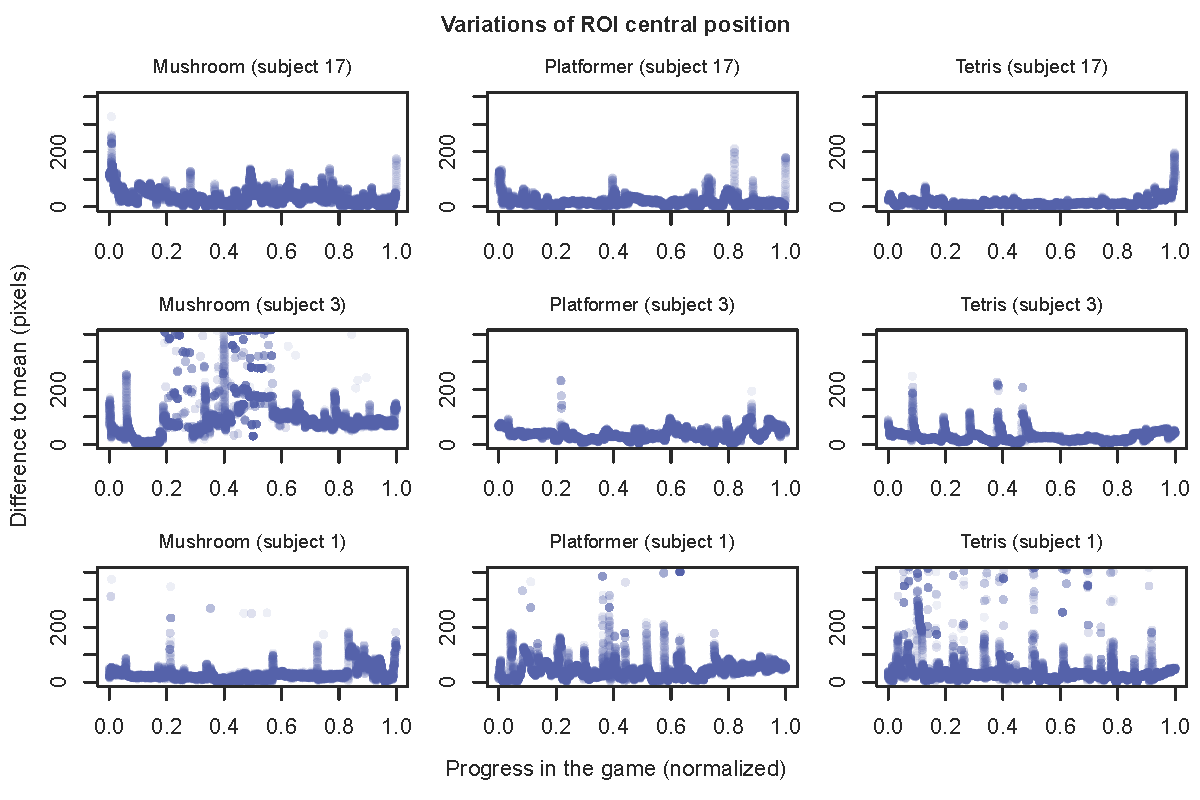
\includegraphics[width=\textwidth]{figures/variation-roi-center.png}
\caption{Variations of distance of the ROI central position for subjects 17 (low estimation errors), 3 (moderate to high estimation errors) and 1 (high estimation errors) during their gaming sessions. Values were subtracted from session mean to facilitate analysis and comparison among different games/subjects.}
\label{fig:chart-roi-anomalies-center}
\end{figure}

Figure \ref{fig:chart-roi-anomalies-center} illustrates some of the patterns observed in the investigation of the distance of the ROI central position. Each row in the figure contains three charts showing the variations of the ROI central position along the gaming sessions of a given subject. The first row contains the investigation of subject 17, who presented, for all his/her gaming sessions combined, -0.33 for $M_e$ ($SD_e$ 1.4) and 1.39 for RMSE (low estimation errors). The second row shows subject 3, who presented 11.47 for $M_e$ ($SD_e$ 16.47) and 19.62 for RMSE (moderate to high estimation errors). Finally the third row shows subject 1, who presented 15.94 for $M_e$ ($SD_e$ 28.5) and 31.96 for RMSE (high estimation errors).

The estimations performed on subject 17 were significantly accurate and the charts regarding the variation of the ROI central position show a stable progression along all gaming sessions. The distance variation (y-axis) remains mostly concentrated within the interval of [0, 100] pixels for all games, which suggest the subject presented few or short movements during gaming sessions. Subject 3 also presented low variation in the Platformer and the Tetris game, however there is a significant variation in the ROI central position in the Mushroom gaming session. The chart indicates significant distance variations of the ROI that are above 200 pixels in a certain period of the game. Finally subject 1 presents high variations in the ROI distance in all gaming sessions, as demonstrated by points above the 200 pixels mark regarding the difference to mean. The Tetris game, in special, present distance variations above 200 pixels during almost the whole session.

\begin{figure}[!h]
\centering
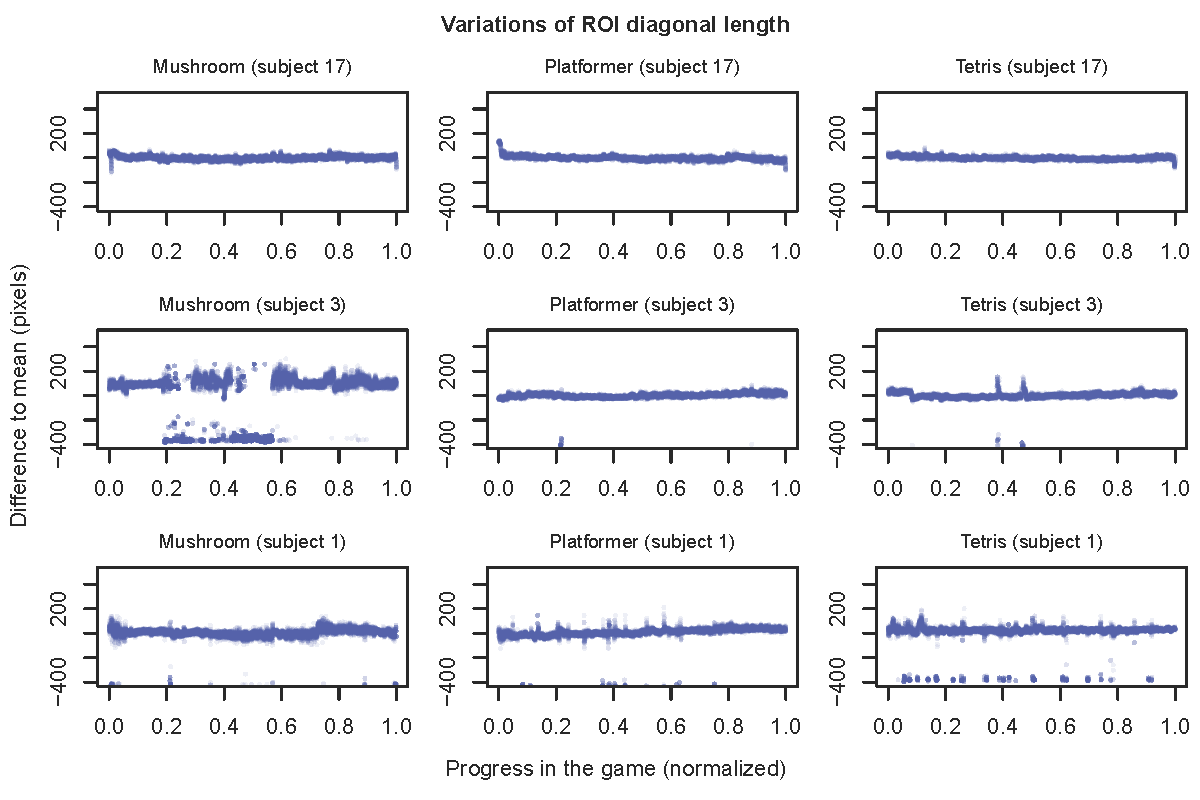
\includegraphics[width=\textwidth]{figures/variation-roi-diagonal.png}
\caption{Variations of ROI diagonal length for subjects 17 (low estimation errors), 3 (moderate to high estimation errors) and 1 (high estimation errors) during their gaming sessions. Values were subtracted from session mean to facilitate analysis and comparison among different games/subjects.}
\label{fig:chart-roi-anomalies-diagonal}
\end{figure}

Figure \ref{fig:chart-roi-anomalies-diagonal} illustrates the same subjects regarding the investigation of the variations of the ROI diagonal length. Similarly to the variations of the ROI central position, the variation of the ROI diagonal length (y-axis) is lower for subject 17 (first row of charts in the figure), since the majority of the values are close to zero. Subject 3 also presents low variations in the ROI diagonal length during the Platformer and the Tetris game, however there are significant changes in the ROI size during a period in the Mushroom game. In such period, the length of the ROI diagonal is negative, i.e. -400 pixels, which indicates the size of the detected ROIs for those frames was smaller than the mean ROI diagonal length. It could be caused by a wrongly detected face (false-negative), for instance. Finally subject 1 presents, to some extent, variations of the ROI diagonal length during the majority of his/her gaming sessions. Those constant variations could be caused by the inability of the face tracking algorithm to stably and continuously detect the subjects face along the frames of the video. The chart shows a distribution of values along the zero mark regarding difference to mean, however they are more spread than those of subject 17, for instance, which indicates higher instability of the ROI size/detection for subject 1. In the Tetris session of subject 1, for instance, there are extreme variation in the ROI diagonal length with values close to -400 pixels, similarly to the ones of subject 3 in the Mushroom game. Such extreme variation could also be explained by a wrongly detected face area during those frames.

An inspection of the videos of subjects with patterns similar to the ones of subjects 3 and 1 revealed sensitive amount of movement and facial activity, including occlusion of the face by the subject's hand, as illustrated by Figure \ref{fig:face-variation}. Any facial occlusion influences the face tracking algorithm used (Viola\&Jones), since it might wrongly detect the face position or do not detect it at all. A flawed face detection step affects the extraction of the plethysmographic signal, because noise is extracted along with the raw signal, making the rPPG technique unable to separate it properly.

Despite the efforts to create games that prevented face occlusion by the subject's hand, such behavior seems to be natural in boring situations. Both Mushroom and Tetris games were more likely to allow players to place a hand in the face to express boredom, since the games could still be played with a single hand when the gameplay speed was not elevated. The Platformer game, on the other hand, is less likely to allow players to use only a single hand to play, which reduced chances of face oclusion inferering with the face tracking algorithm. This could also explain why estimations made during the Platformer game were more accurate than those performed during the other two games. Those extreme cases with facial occlusion are probably affecting the error rates in the analysis, producing less accurate estimations. Such extreme and flawed cases could have removed from the analysis, however the aim is to test how the selected rPPG technique performs in natural gaming situations. A dataset with untreated videos of gaming sessions with natural interactions might produce sub-optimal HR estimations, however it is the understanding that stressing the rPPG technique with less artificial videos provides researchers with insights about possible problems and accuracy limits of such tool.

\begin{figure}
\centering
  \begin{subfigure}[b]{0.5\textwidth}
    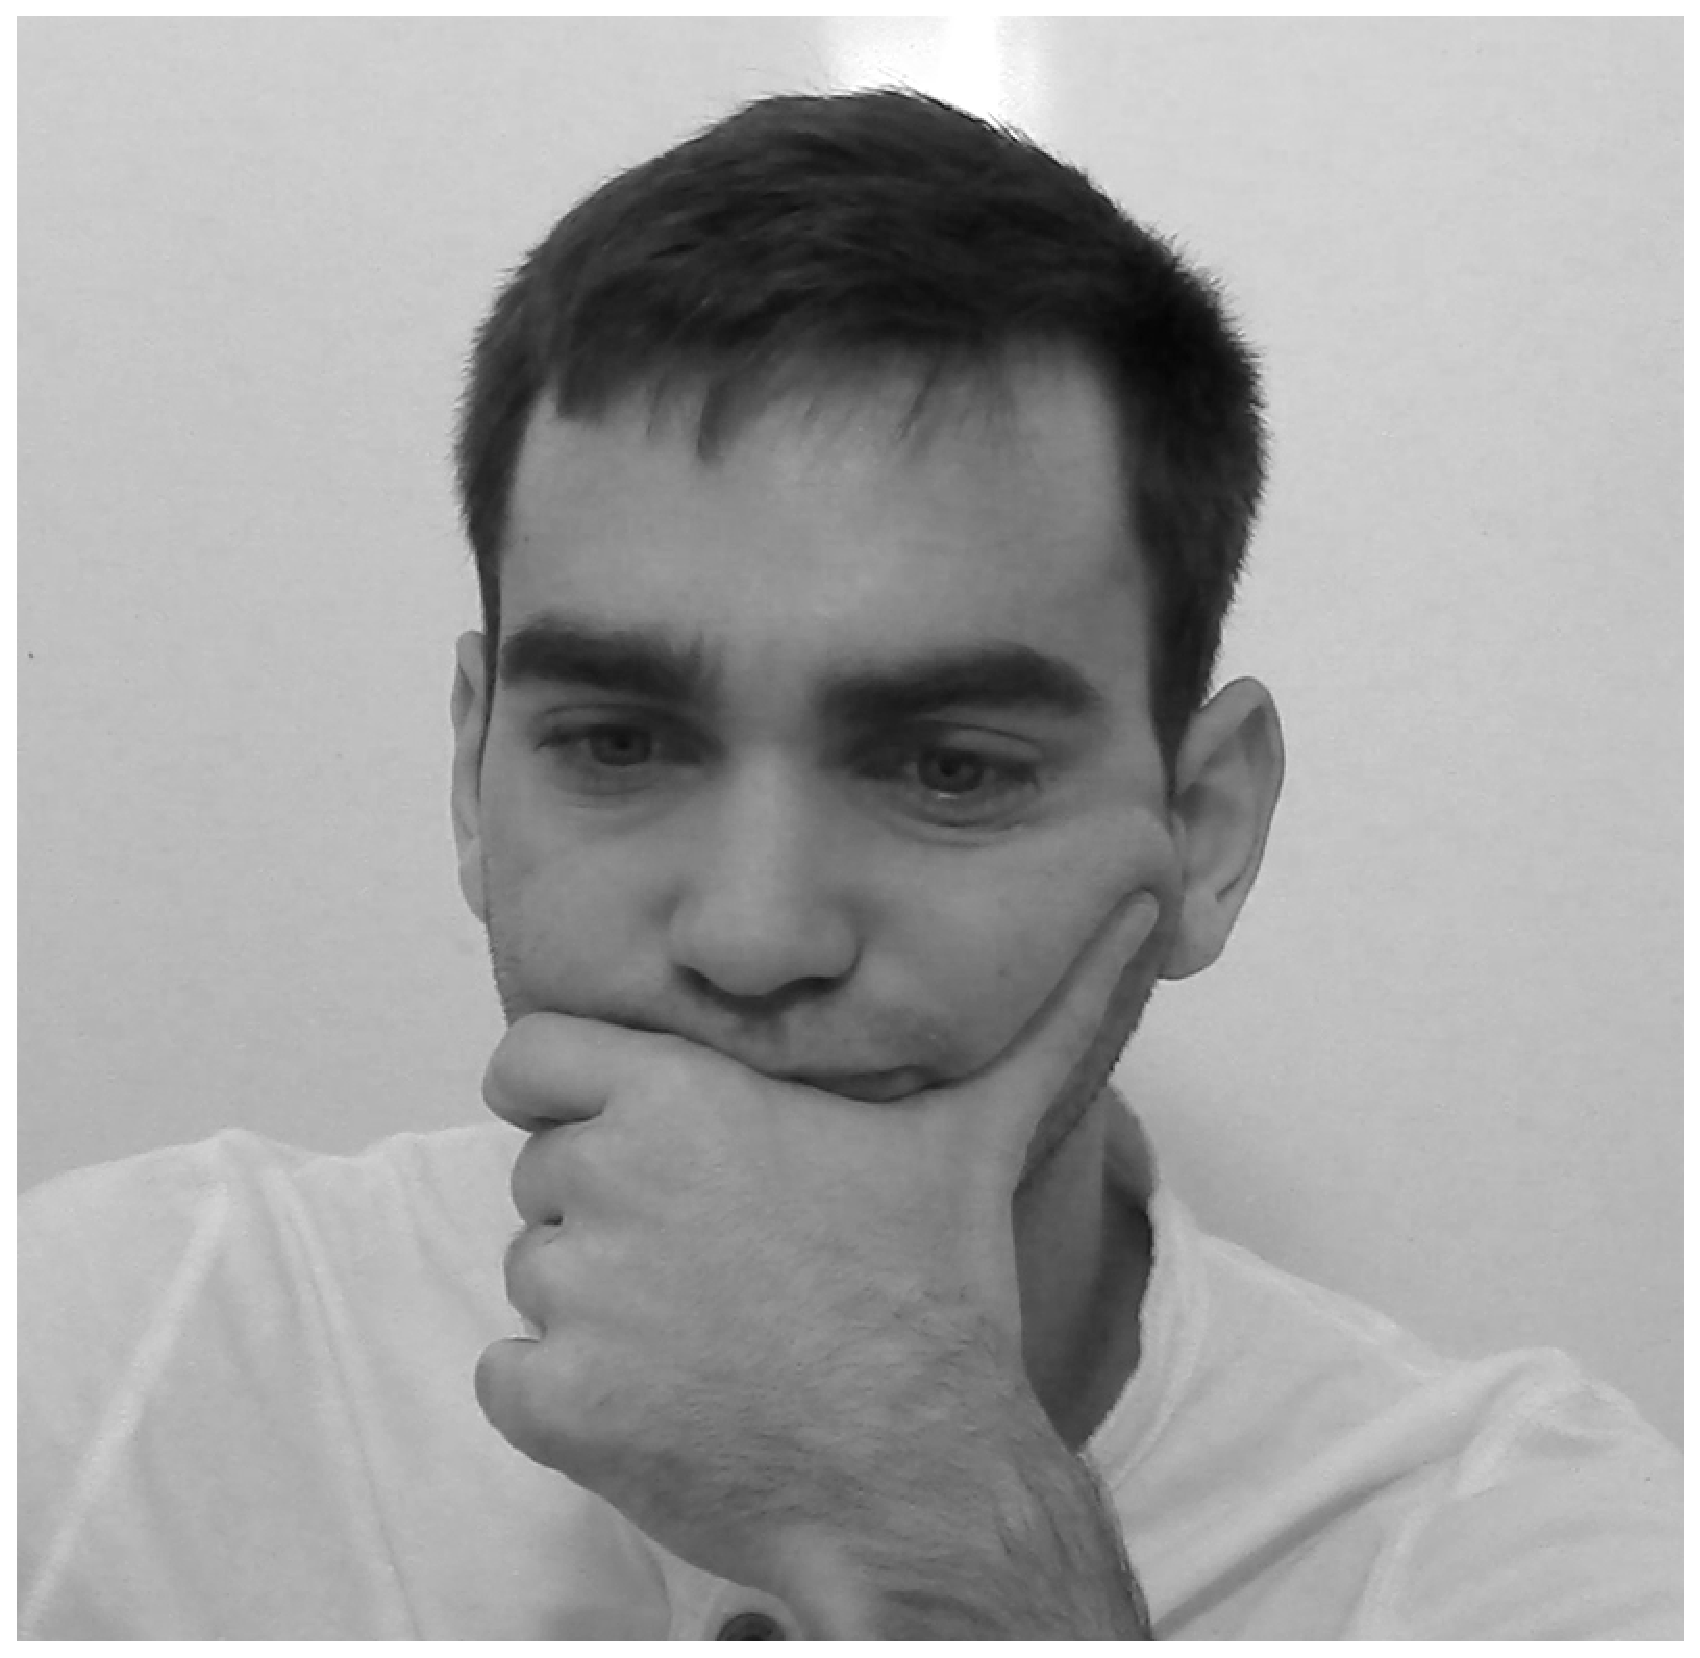
\includegraphics[width=0.95\textwidth]{figures/face-occlusion}
    \caption{}
    \label{fig:face-occlusion}
  \end{subfigure}%
  \begin{subfigure}[b]{0.5\textwidth}
    \centering
    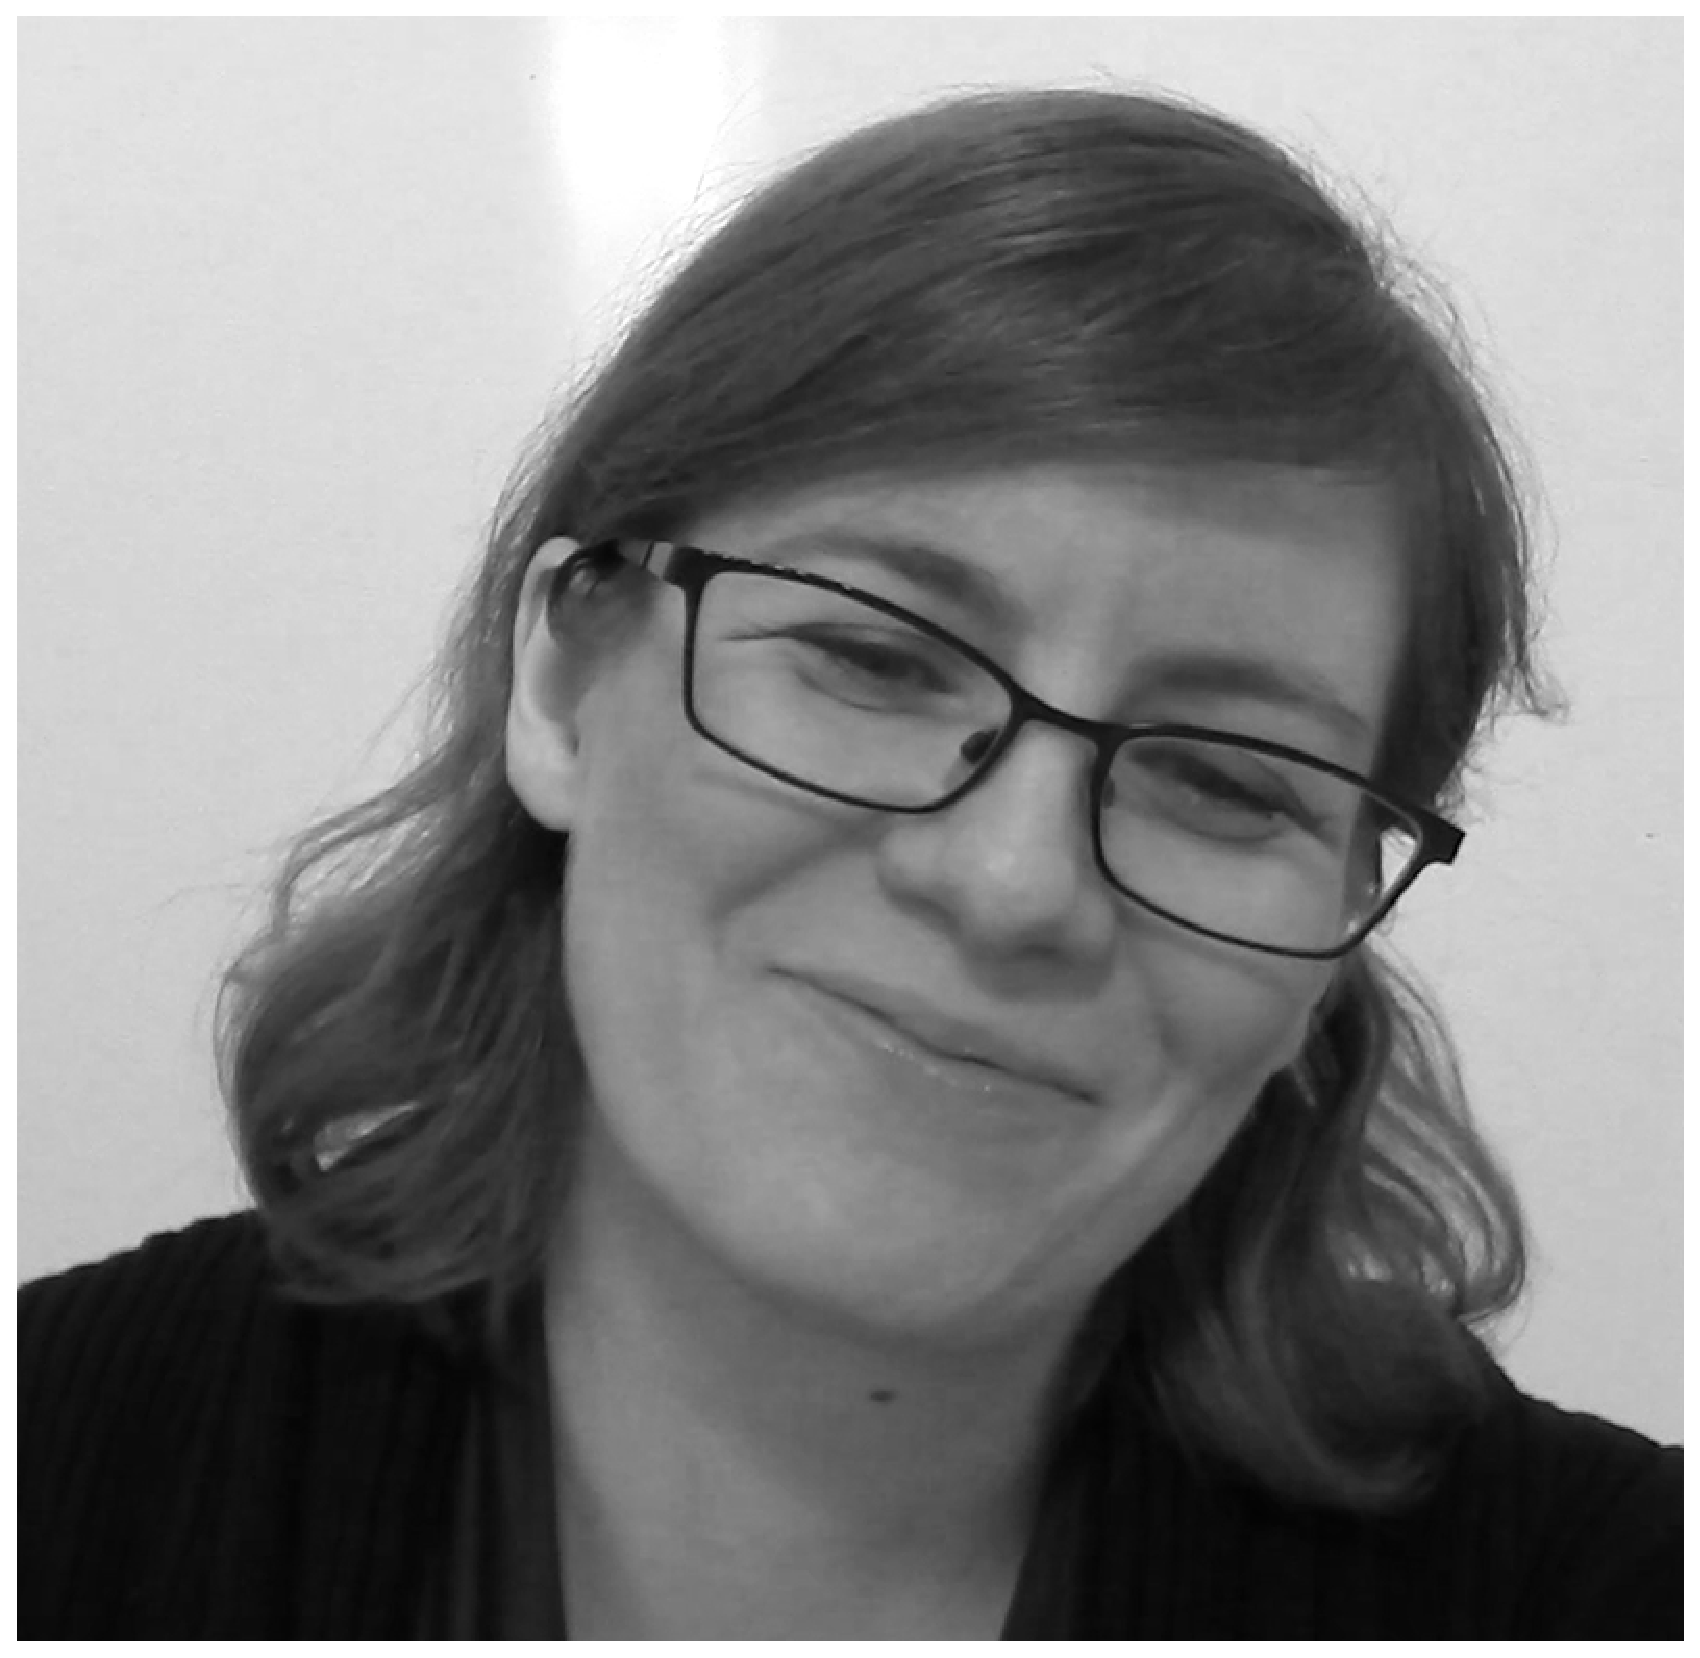
\includegraphics[width=0.95\textwidth]{figures/head-tilt}
    \caption{}
    \label{fig:head-tilt}
  \end{subfigure}
  \caption{Examples of body movement and facial activity during gaming sessions. (a) Partial face occlusion by subject's hand; (b) Head tilt and movement during laugh action.}
  \label{fig:face-variation}
\end{figure}

It is possible to speculate that the variations regarding movement and size of the ROI, which directly influence estimation accuracy of the rPPG technique, seem to be connected to the unique behavior of each user as well. As illustrated by Figures \ref{fig:chart-roi-anomalies-center} and \ref{fig:chart-roi-anomalies-diagonal}, subjects present different movement patterns. Previous analysis of the videos indicates significant differences regarding facial activities among subjects \parencite{bevilacqua2016variations}. It strengthens the idea of a user-tailored model able to deal with such peculiarities, which is more likely to produce better estimations. A method that operates its estimations based on the average user behavior is prone to be significantly affected by specific user behavior outside the expected mean pattern, causing skewed distribution of estimation errors such as the ones presented on Figure \ref{fig:chart-hists} regarding $M_{eRate}$ and RMSE.

%\subsection{Limitations}

%Some limitations of the experimental procedure and analysis should be noted. The 1-minute long duration of each video segment used for the estimation of HR may affect the results. The ideal length of the video segment used for estimation (called window size) is not agreed upon in the literature \parencite{rouast2016remote}. In general, it depends on the characteristics of the rPPG technique being applied as well as the hardware configuration, such as camera framerate \parencite{roald2013estimation}. We selected a 1 min analysis window based on the information of the original work by \textcite{poh2011advancements}. Additionally our experimental procedure consists of games whose difficulty level changes every 1 minute, so that value is aligned with the window size used for HR estimation. As previously described, the statistical nature of ICA, part of the selected rPPG employed in the experiment, demands longer video samples to produce accurate results. The longer the video, however, the higher the chances of subject motion, which increases noise. A trade-off between the duration of the video segments and the estimation accuracy could be better investigated. Our experimental setup used an external light source to minimize noise caused by changes in illumination, which should narrow the estimation error to causes as subject movement and/or facial activity. It is likely, however, that other factors might impact the estimation accuracy, such as facial hair, e.g. beard and hair over the forehead area, use of glasses, and skin color.

\subsection{Conclusions}

Overall the estimation of the rPPG was feasible, showing mean estimation error of 2.99 bpm (SD 18.83 bpm), RMSE of 19.03 bpm and a positive and medium strength Pearson correlation of $r=0.43$, $p < 0.001$. On average, the estimation error of the rPPG technique was up to 10.31\% of the expected value calculated from ground truth. Additionally the exploratory investigation regarding factors that impacted the accuracy of the rPPG technique, such as variations in the region of interest (ROI) used to remotely extract the HR signal, suggest factors connected to the type of the game being played and the unique behavior of each subject influenced the estimations. Among the causes of such influence were identified body movement, e.g. head tilt and rotation, and facial occlusion by subjects hand.

%Our results provide researchers with information related to the reliability of a remote HR measurement technique when applied to the context of games research. We believe our experimental setup is a novel approach in the exploration of the accuracy of rPPG-estimated HR readings of subjects in a gaming context. To the best of our knowledge, our experiment is the first to measure the accuracy of an rPPG technique with the use of three boredom/stress-inducing games with subjects behaving naturally. Future work involves investigation of facial activity as well as body movement as a complementary source of information to be used along with remote HR estimation in a multimodal analysis for the identification of stress and boredom in games. As demonstrated, subject movement affects rPPG estimations, however it is an inherent characteristic of a gaming session with natural behavior. We will analyse the use of such signals in a user-tailored approach, focusing on the particular behavior of each user instead of the average pattern.


\chapter{Experiment 2: validation of remote detection of emotions}
\label{ch:experiment2}

The experiment described in this chapter, the second one conducted, aimed at validating the proposed approach for remote detection of emotions, described in the objectives of this thesis (see Section \ref{sec:contributions}, on page \pageref{sec:contributions}). The approach uses remotely acquired signals, namely heart rate (HR) and facial actions (FA), to create a user-tailored model, i.e. trained neural network, able to detect emotional states of boredom and stress of a given subject. The approach is composed of two phases: training (or calibration) and testing. In the training phase, the model is trained using a user-tailored approach, i.e. data from subject $S_a$ playing 3 calibration games (Mushroom, Platformer and Tetris) is used to create model $M_a$. The result of the training phase is a user-tailored model, i.e. model $M_a$, which is a trained neural network aimed to be used on subject $S_a$. The testing phase happens in a game session involving subject $S_a$ playing any ordinary, non-calibration game, e.g. Super Mario. During the testing phase, subject's $S_a$ signals are remotely acquired and fed into the previously trained model $M_a$, which outputs the estimated emotional state of subject $S_a$ for that particular testing game.

In summary, this experiment is intendeded to answer the following research question:

\begin{fquote}
How accurate is an emotion detection approach that uses remotely acquired signals, i.e. heart rate and facial actions, as input of a machine learning model, i.e. neural network, that was trained on a user-tailored basis (one subject produces one model) using calibration games as emotion elicitation?
\end{fquote}

The overall hypothesis of this experiment is that the accuracy of the model during the testing phase is acceptable. It validates and proves the proposed approach as feasible. The next sections present the experiment, detailing the participants, structure and results, followed by a discussion and a conclusion.

%%%%%%%%%%%%%%%%%%%%%%%%%%%%%%%%%%%%%%%%%%%%%%%%%%%%%%%%%%%%%%%%%%%%%%%%%%%%%%%%%%%%%%%
\section{Participants}
%%%%%%%%%%%%%%%%%%%%%%%%%%%%%%%%%%%%%%%%%%%%%%%%%%%%%%%%%%%%%%%%%%%%%%%%%%%%%%%%%%%%%%%

Sixty two ($N=62$) adult participants of both genders (38.7\% female, 61.3\% male) with different ages (19 to 66, mean 27.2, SD 7.2) and different gaming experience gave their informed and written consent to participate in the experiment. The study population consisted of staff members and students of the University of Sk\"ovde, as well as citizens of the community/city.

When asked how skilled subjects believe they are at playing video games, 6 subjects (9.7\%) reported no skill, 19 (30.6\%) reported not very skilled, 25 (40.3\%) reported moderately skilled and 12 (19.9\%) reported very skilled. When asked the number of hours per week they had played any type of video game over the last year, 25 subjects (40.3\%) reported more than 10, 7 (11.3\%) reported 5 to 10, 6 (9.7\%) reported 3 to 4, 5 (8.1\%) reported 1 to 3, 10 (16.1\%) reported 0 to 1, and 9 (14.5\%) reported no activity.

Those numbers indicate that the sample population has a diversity of ages, gaming experience and playing frequency. Such diversity provides heterogeneous data that allows a more realistic and broad analysis of the proposed method.

%%%%%%%%%%%%%%%%%%%%%%%%%%%%%%%%%%%%%%%%%%%%%%%%%%%%%%%%%%%%%%%%%%%%%%%%%%%%%%%%%%%%%%%
\section{Method}
%%%%%%%%%%%%%%%%%%%%%%%%%%%%%%%%%%%%%%%%%%%%%%%%%%%%%%%%%%%%%%%%%%%%%%%%%%%%%%%%%%%%%%%

The following sections present the experiment structure and the methods employed to collect and analyse data.

%%%%%%%%%%%%%%%%%%%%%%%%%%%%%%%%%%%%%%%%%%%%%%%%%%%%%%%%%%%%%%%%%%%%%%%%%%%%%%%%%%%%%%%
\subsection{Experimental procedure}

Subjects were seated in front a computer, alone in the room, while being recorded by a camera and measured by a heart rate sensor, as illustrated in Figure \ref{fig:experiment2-setup}. The camera was attached to a tripod placed in front of the subjects at approximately 0.6m of distance; the camera was slightly tilted up. A spotlight, tilted 45$^{\circ}$ up, placed at a distance of 1.6m from the subject and 45cm higher than the camera level, was used for illumination; no other light source was active during the experiment.

\begin{figure}[ht]
\centering
  \begin{subfigure}[b]{0.5\textwidth}
    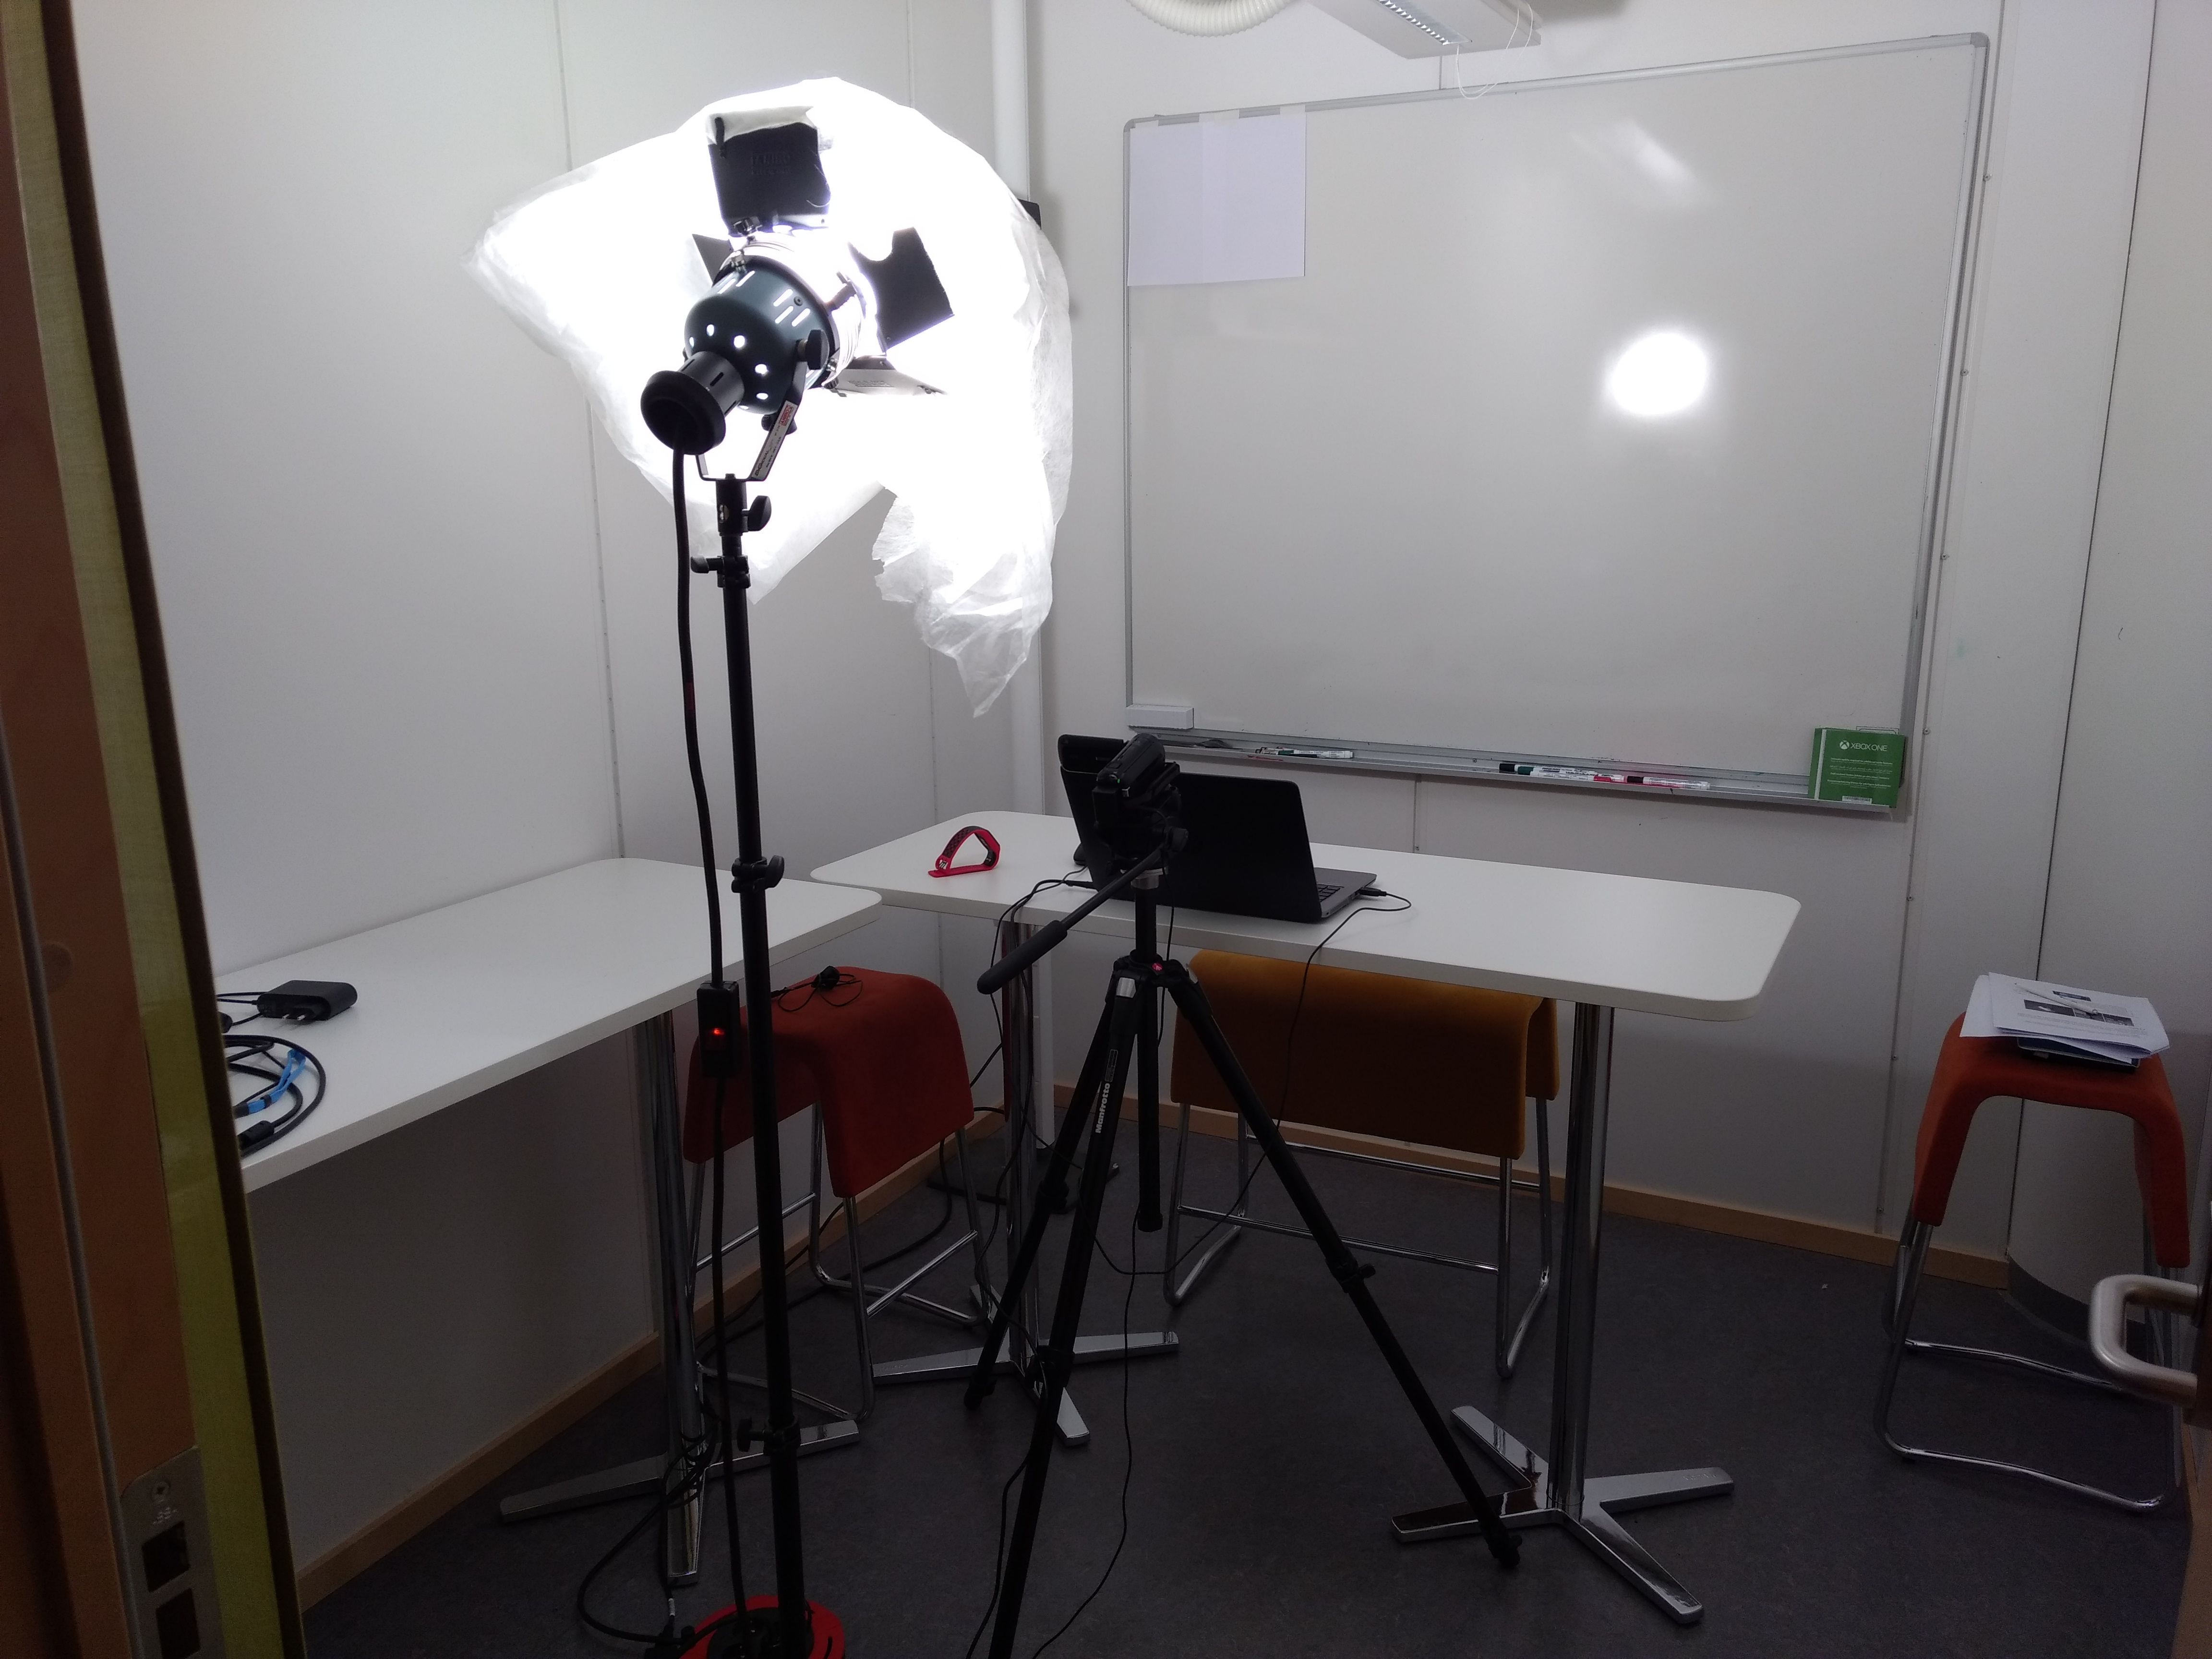
\includegraphics[width=0.95\textwidth]{figures/experiment2-setup-overall}
    \caption{}
    \label{fig:experiment2-setup-overall}
  \end{subfigure}%
  \begin{subfigure}[b]{0.5\textwidth}
    \centering
    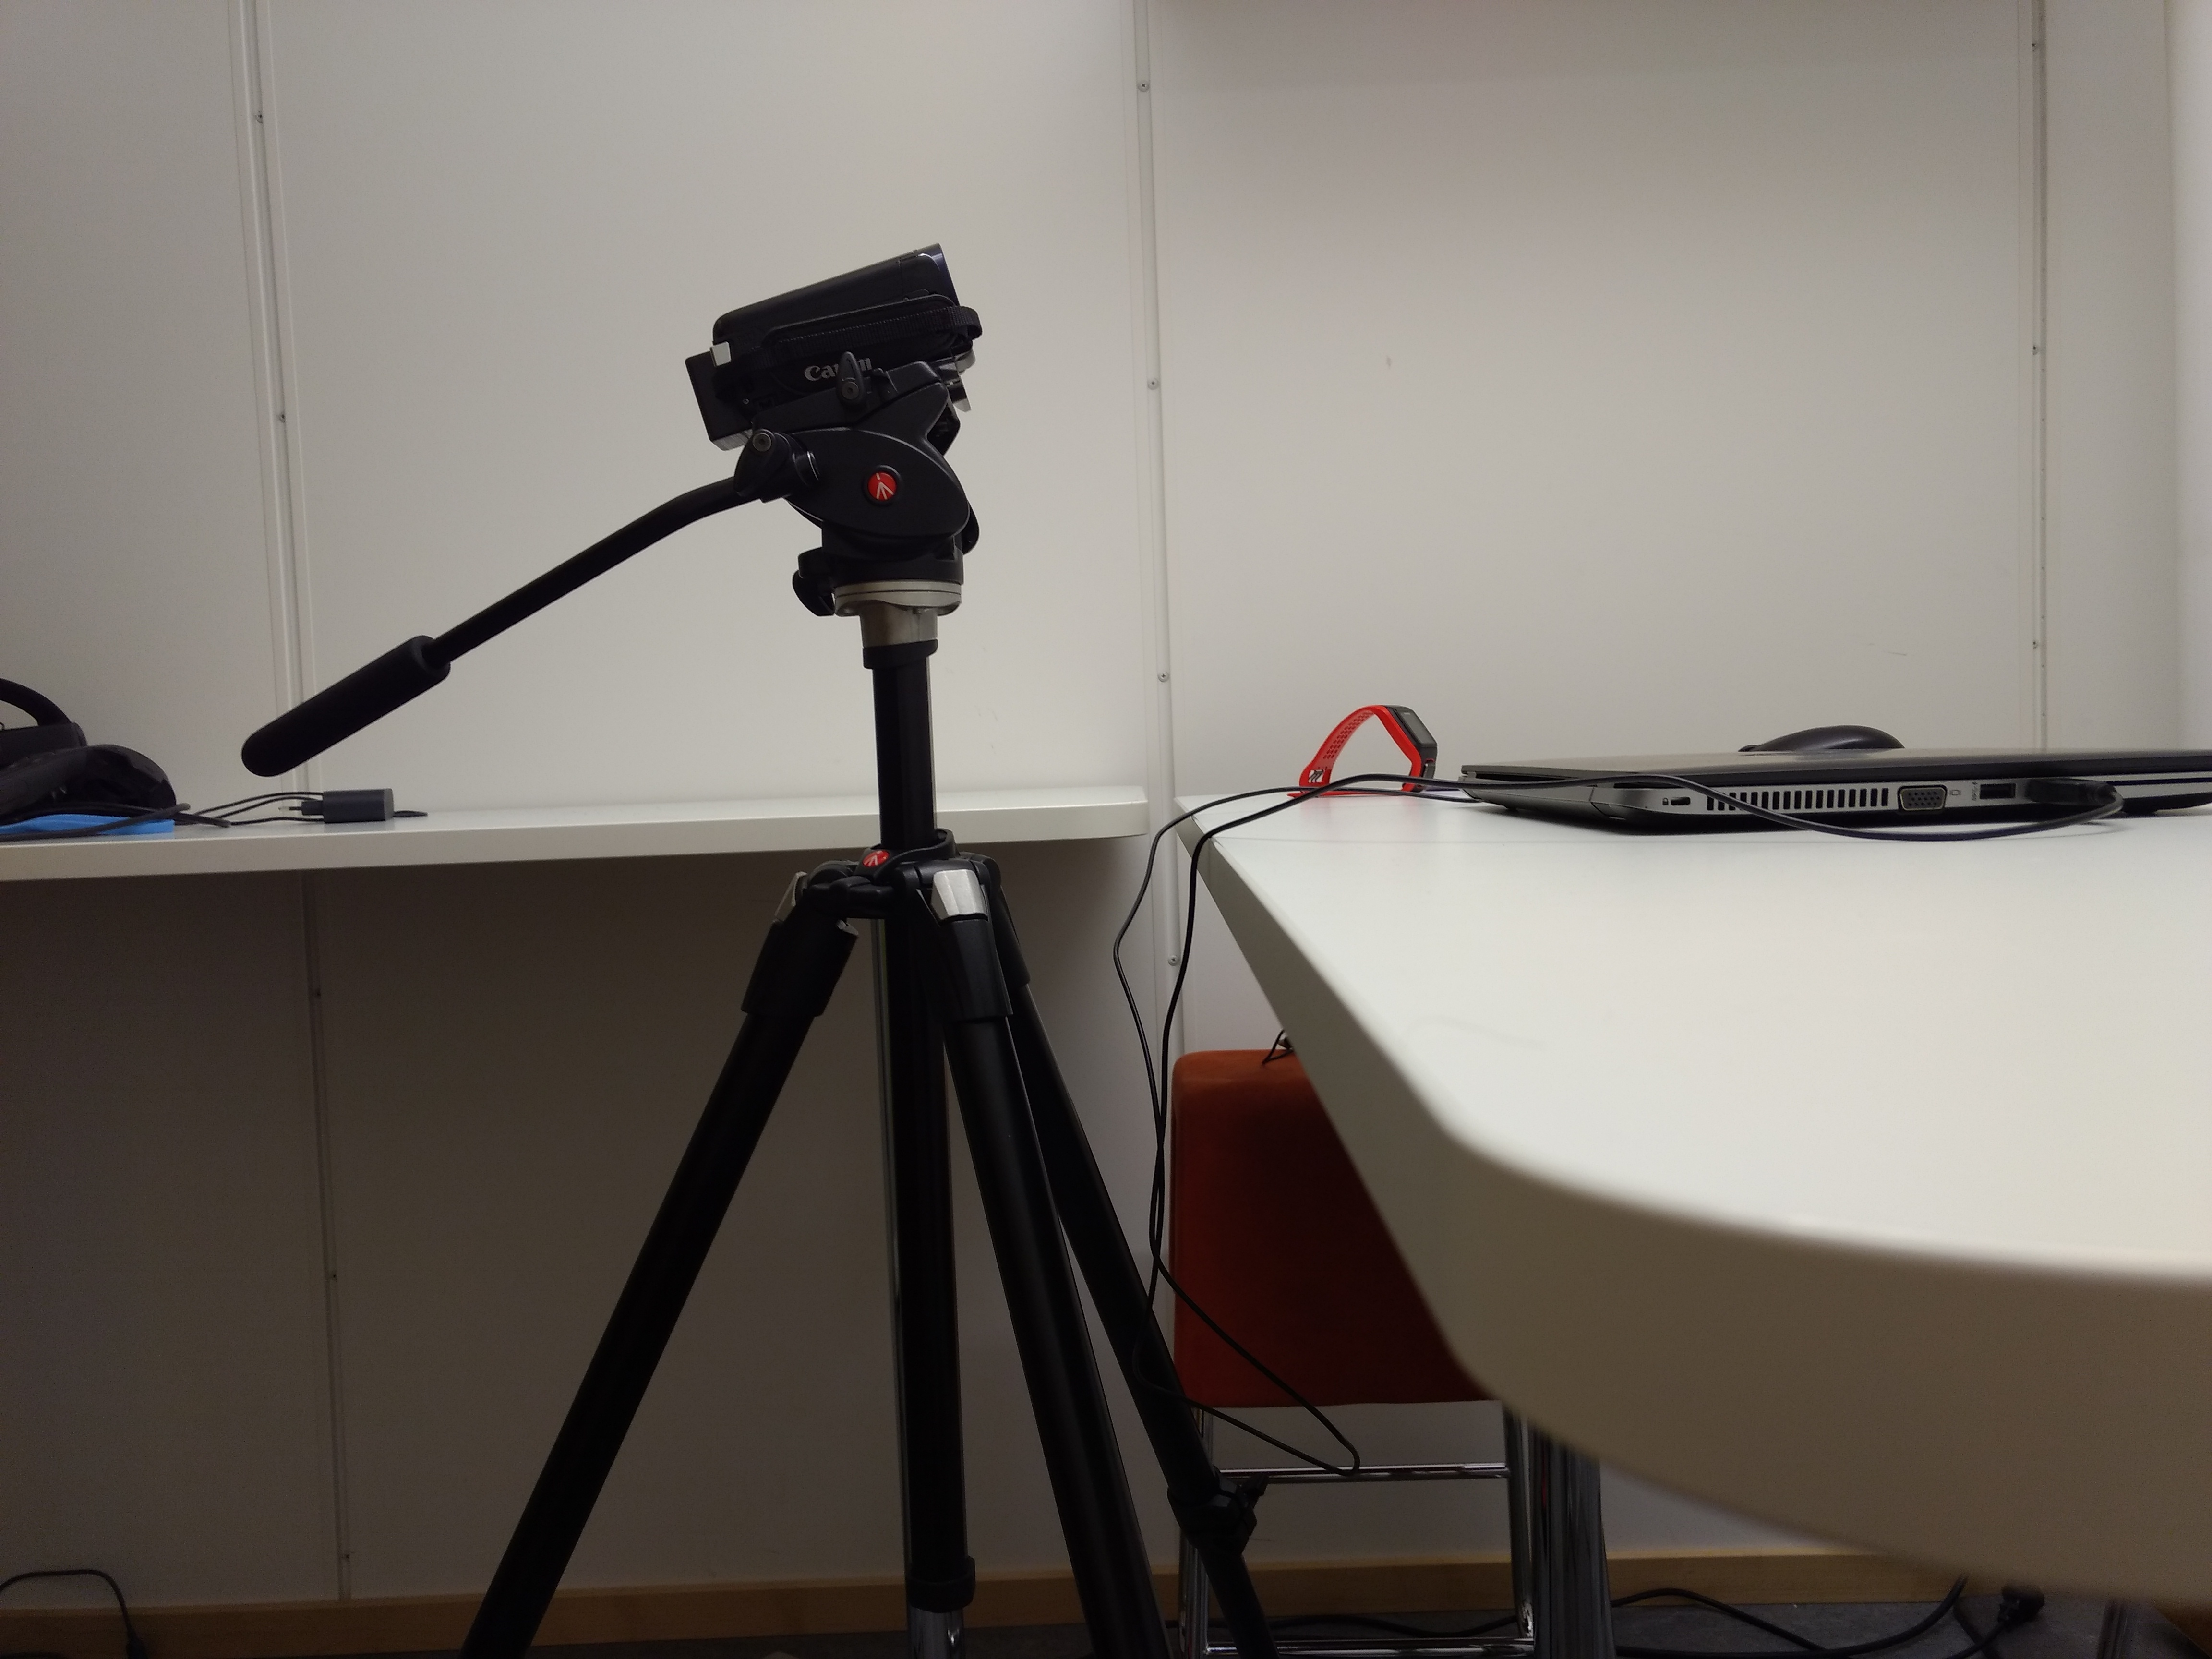
\includegraphics[width=0.95\textwidth]{figures/experiment2-setup-camera}
    \caption{}
    \label{fig:experiment2-setup-camera}
  \end{subfigure}
  \caption{Experiment setup. (a) Position of equipment, showing computer, camera, and external light source. (b) Highlight of the video camera and it angulation.}
  \label{fig:experiment2-setup}
\end{figure}

Participants were each recorded for about 45 minutes on average during two (uninterrupted) parts of the experiment, i.e. calibration and testing phase, as illustrated by Figure \ref{fig:experiment2-parts}. The calibration phase, aimed at gathering data for training a user-tailored model, subjects played 3 games (described in the next section). Each of those games was followed by a questionnaire related to the game and stress/boredom levels. Games were also followed by a 138 seconds rest period where subjects listened to calm classic music. The testing phase, aimed at gathering data to test the accuracy of the user-tailored model, subjects played 7 levels of an evaluation game, i.e. Infinite Mario (described in details in the next sections).

In the calibration phase, games were carefully designed to start with a difficulty level that is significantly low, which is expected to lead the player to an immediate state of boredom. As time progresses, the difficulty level increases linearly. As the difficulty level continues to rise, at certain point the game will become too hard to be managed by the subject, which eventually results in a ``game over" state. Moments before that point the subject should reach his/her stress peak during gameplay. It is expected that each player experiences three distinct states during the gameplay of each game: boredom (low challenge/stress) at the beginning, flow (ideal challenge/stress) after the beginning and before the final moments, and stress (high challenge/stress) at the end. The order in which the games were played was randomized among subjects during the calibration phase of the experiment.

\begin{figure}[ht]
  \centering
  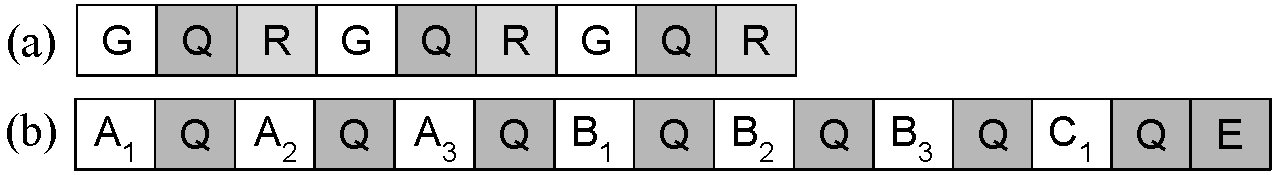
\includegraphics[width=\textwidth]{figures/experiment2-parts}
  \caption{Experiment setup}
  \label{fig:experiment2-parts}
\end{figure}

In the testing phase, subjects played 3 batches of Infinite Mario levels: batches $A$, $B$ and $C$ containing 3, 3 and 1 level each, respectively. Except for level $C_1$ in batch $C$, levels in batches $A$ and $B$ were designed to present an increase in difficulty within the batch, so levels $A_1$ and $B_1$ are expected to be less difficult/challenging than levels $A_3$ and $B_3$, for instance. Similarly levels in batch $B$ were designed to be more challenging than levels in batch $A$, also following an increase in difficulty. Consequently levels $B_i$ are expected to be slightly more difficult/challenging than levels $A_i$. This pattern is intended to mimic the balance curve of a commercial game, where levels, and game parts, commonly tend to increase its difficulty as the game story progresses. In order to ensure subjects would experience some level of boredom during the testing phase, which is required for the evaluation of the proposed method, levels $B_1$ and $C_1$ were designed using Mario's auto-scrolling camera mechanics. In such configuration, the player has no control of the speed of the level. This mechanic is expected to induce boredom, since the player experienced allegedly challenging (and fun) levels previously and is now unable to move using any desired speed. After each level, subjects answered a questionnaire about how bording/stressful the game level just played was. The order in which the levels were played was not randomized among subjects during the testing phase of the experiment. As a consequence, all subjects played the evaluation game in the same order: levels $A_1$ to $A_3$, followed by levels $B_1$ to $B_3$, finally followed by level $C_1$.

After subjects finished playing the last level in the testing phase, i.e. level $C_1$, they answered a final questionnaire about age and gaming experience/profile. Before starting the experiment, participants received instructions from a researcher that they should play a few games, answer questionnaires after each game and rest when instructed; they were told that their gaming performance was not being evaluated, that they should not give up in the middle of the games, that a time limit exists for some levels to prevent them from playing for too long, and that they should remain seated during the whole process.

The following sections explain in details each one of the games used in the two parts of the experiment.

\subsubsection{Calibration games}

The three games\footnote{Source code available at: https://fernandobevilacqua.com/link/phd-experiment2} used as calibration games in the experiment were 2D and casual-themed, played with mouse or keyboard in a web browser. The games were carefully designed to provoke boredom at the beginning and stress at the end, with a linear progression between the two states (adjustments of such progression are performed every 1 minute). The game mechanics were chosen based on the capacity to fulfill such linear progression, along with the quality of not allowing the player to instantly kill the main character (by mistake or not), e.g. by falling into a hole. The mechanics were also designed/selected to ensure that all subjects would have the same game pace, e.g. a player must not be able to deliberately control the game speed based on his/her will or skill level.

The Mushroom game, shown in in Figure \ref{fig:mushroom-platformer-tetris} (left), is a puzzle where the player must repeatedly feed a monster by dragging and dropping mushrooms. Boredom is induced with fewer mushrooms to deal with and plenty of time for the task, while stress is induced with increased number of mushrooms and limited time to drag them. The Platformer game, shown in in Figure \ref{fig:mushroom-platformer-tetris} (middle), is a side-scrolling game where the player must control the main character while collecting hearts and avoiding obstacles (skulls with spikes). Boredom is induced with a slow pace and almost no hearts or obstacles appearing on the screen, while stress is induced with a faster pace, several obstacles, and almost no hearts to collect. Finally the game Tetris, shown in Figure \ref{fig:mushroom-platformer-tetris} (right), is a modified version of the original Tetris game. In our version of the game, the next block to be added to the screen is not displayed and the down key, usually used to speed up the descendant trajectory of the current piece, is disabled, preventing players from speeding up the game. Boredom is induced by slow falling pieces, while stress is induced by fast falling pieces. All games used the same seed for random calculations, which ensured subjects received the same sequence of game elements, for example, pieces in Tetris. For a detailed description of the games, refer to Section \ref{sec:experiment1-games-elicitation} (on page \pageref{sec:experiment1-games-elicitation}).

\subsubsection{Evaluation game (Infinite Mario)}

%Pedersen, C.; Togelius, J. & Yannakakis, G. N. Modeling player experience in Super Mario Bros. 2009 IEEE Symposium on Computational Intelligence and Games, IEEE, 2009, 132-139

%Pedersen, Christopher, Julian Togelius, and Georgios N. Yannakakis. "Modeling player experience for content creation." IEEE Transactions on Computational Intelligence and AI in Games 2.1 (2010): 54-67.

%Shaker, N.; Asteriadis, S.; Yannakakis, G. N. & Karpouzis, K. A game-based corpus for analysing the interplay between game context and player experience. Affective Computing and Intelligent Interaction, Springer, 2011, 547-556

% Shaker, N.; Yannakakis, G. N. & Togelius, J. Feature analysis for modeling game content quality. 2011 IEEE Conference on Computational Intelligence and Games (CIG'11), IEEE, 2011, 126-133

The game used in the evaluation phase of the experiment is a modified version\footnote{The version of the game used in the experiment is a HTML5, web-based version built by Robert Kleffner, available at: https://github.com/robertkleffner/mariohtml5. Robert ported to HTML5 the original Java version created by Markus Persson. Source code of both versions, Robert's and Markus', are in the public domain. The source code of the final version used in this experiment is available at: https://fernandobevilacqua.com/link/phd-experiment2} of Markus Persson's Infinite Mario, a public domain clone of Nintendo's platform game \textit{Super Mario Bros}. In the case of this experiment, the game is played with a keyboard in a web browser. Infinite Mario has been widely mentioned in the literature, including studies involving modeling of player experience \parencite{pedersen2009modeling,pedersen2010modeling,shaker2011game} and detection of affective states \parencite{shaker2011feature}.

\begin{figure}[h]
  \centering
  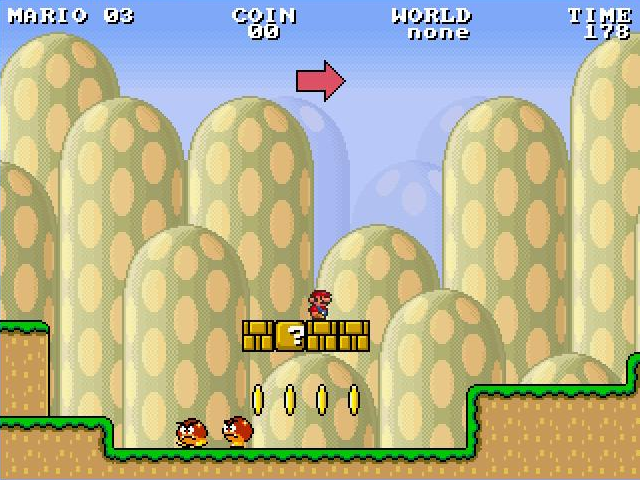
\includegraphics[width=.32\textwidth]{figures/infinite-mario}\hfill
  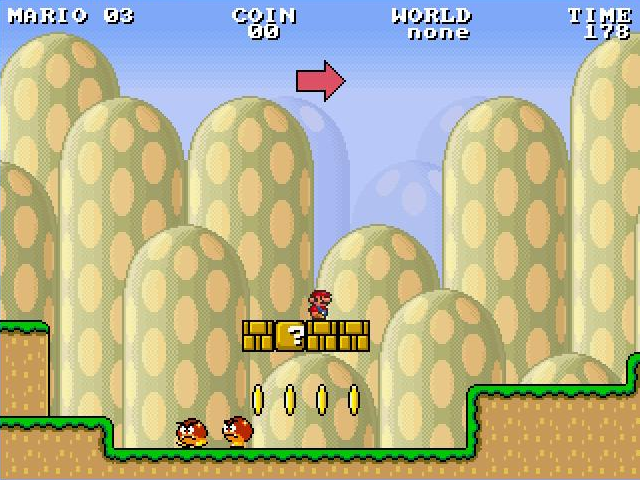
\includegraphics[width=.32\textwidth]{figures/infinite-mario}\hfill
  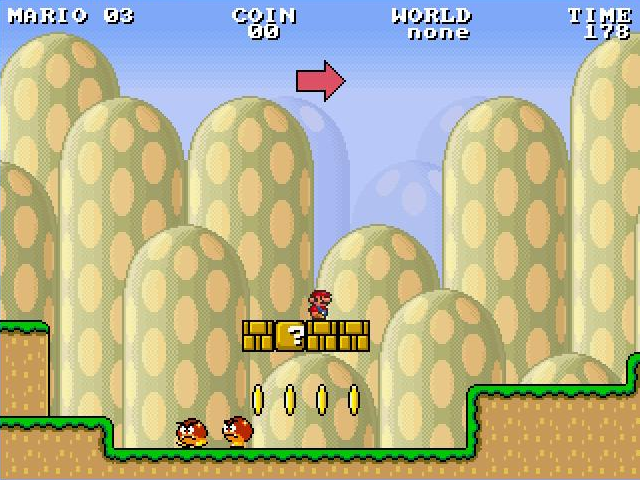
\includegraphics[width=.32\textwidth]{figures/infinite-mario}
  \caption{Infinite Mario}
  \label{fig:experiment2-infinite-mario}
\end{figure}

The gameplay in Super Mario, consequentially in Infinite Mario as well, consists of controling the main character, Mario, along the level. Mario can move left or right, jump, run, duck, and throw fireballs (if the power-up \textit{Flower} has been collected). The objective of the game is to complete each level, which is accomplished by traversing it from left to right until the ``end of level" checkpoint is reached. Mario can be in three different states: small, big, and power-up. If Mario is small, any interaction with enemies differently from landing on top of them after a jump results in Mario getting killed immediately. If Mario is big, the same ``wrong" interaction with enemies causes Mario to get hurt and transform into the small state. If Mario is in the power-up state, the ``wrong" interaction with enemies causes Mario to get hurt and transform into the big state. Consequently keeping Mario in the big or power-up state is a strategic advantage to prevent kills that likely calms the player, i.e. relaxed. On the other hand keeping Mario in the small state is less benefical since mistakes are fatal, so it is likely that players feel anxious/stressed in such conditions.

Along the level, Mario might encounter enemies, which can be killed or ignored. Mario can kill enemies by jumping and landing on top of them, which is rewared with score points. Some enemies, e.g. Koopa Troopa (a sort of turtle), leave a shell behind when killed by Mario. The shell can be picked up by Mario and carried around, serving as a weapon when released. Levels might also contain terrain obstacles of varying sizes, e.g. gaps, that must be jumped over. If Mario falls in a gap, he dies immediately. Mario can also find collectable items, i.e. coins and power-ups, or interactable items, e.g. blocks. Mario collects items by touching them, i.e. a collected results in score points. Collectable items might be visible in the level or hidden inside interactable items, e.g. blocks. Mario interacts with blocks by bumping into them from below, e.g. jumping and hitting Mario's head on the bottom of a block destroys it. A destroyed block might give a collectable item as a reward, e.g. coin, \textit{Mushroom} (Mario transitions to big state) or \textit{Flower} (Mario transitions to power-up state).

During the gameplay, on the top of the screen there are information about Mario, the score and the current level. The information includes the number of lives Mario has (to complete that level), the level score, the number of coins collected (collecting 100 coins results in an extra life), the name of the current level, and the amount of time available to complete the level (constantly ticking down). If the time remaining to complete the level reached the 60 seconds mark, a hurry up SFX is played and the background music starts to play in a faster tempo. Unless informed otherwise, all levels start with 3 lives and 200 seconds of available time. Every time Mario dies, the time remaining to complete the level is reset to its initial value, e.g. 200 seconds.

Originally Infine Mario has all its gameplay content, e.g. level design and position of items/enemies, generated procedurally. This behavior is not desired for the experiment, since all subjects should experience the same Mario levels. Additionally subjects should feel stressed and bored in game at some points, so the proposed emotion detection method can be properly evaluted when detecting of such moments. As a consequence, Infinite Mario was adapted and tweaked to fit as an ideal evaluation game in the experiment. Firstly the procedural content generation was contrained by a seed and a set of paramaters that control how content is created, e.g. length of the level, amount and width of terrain obstacles, e.g. gaps and platforms, availability of coins and power-ups, among others. Previous works using Infinite Mario \parencite{pedersen2009modeling,pedersen2010modeling} have shown a correlaction between anxiety and 1) difficulty of jumping, e.g. overcoming obstacles, and 2) gap width. There is also a correlaction between boredom and the width of gaps, i.e. the wider the gap, the less boring the level is. Based on those findings and the guidance provided by game design experts, the Mario levels used in the experiment were adjusted according to the description presented in Table \ref{table:experiment2-mario-levels}. Column \textit{Level} refers to the level name/number. Column \textit{Type} refers to the visual representation of the level. Possible types are \textit{Overground} (open sky and green landscape), \textit{Underground} (closed ceiling, dirt-like environment), and \textit{Castle} (closed ceiling, resempling the interior of a castle). Each level type features different visual elements and background music. Column \textit{Emotion} refers to the expected emotional state most subjects will experience. Finally column \textit{Adjustments} refer to the constraints used to generate the level's content.

\todo{Illustrate level types using provided screenshots.}

\begin{landscape}
\begin{table*}
    \centering
    \caption{Levels of Infinite Mario and adjustments performed to induce a particular emotional state on them.}
    \label{table:experiment2-mario-levels}
    \begin{tabular}[l]{@{}cllp{9.5cm}}
        \hline
            \textbf{Level} & \textbf{Type} & \textbf{Emotion} & \textbf{Adjustments} \\
        \hline
            $A_1$ & Overground  & Any & Reduced number of interactable/collectable items and terrain obstacles; no power-ups; only 2 enemies and 1 gap (with width of Mario himself); Mario starts in big state. \\
            $A_2$ & Underground & Any & Regular number of interactable/collectable items, terrain obstacles, power-ups and enemies. Mario starts in small state. \\
            $A_3$ & Castle      & Stress  & Several gaps (with varying widths); reduced number of interactable items; no collectables/power-ups; several enemies; reduced time to complete level. Mario remains in small state. Mario starts with 5 lives. Available level time is 80 seconds. \\
            $B_1$ & Overground  & Boredom & Auto-scrolling camera; reduced number of interactable/collectable items; few terrain obstacles; no gaps, power-ups, or enemies. Mario remains in big state. \\
            $B_2$ & Underground & Any & Regular number of interactable/collectable items, terrain obstacles, power-ups and enemies. Mario starts in small state. \\
            $B_3$ & Castle      & Stress  & Several gaps (with varying widths); reduced number of interactable items; no collectables/power-ups; several enemies; reduced time to complete level. Mario remains in small state. Mario starts with 5 lives. Available level time is 80 seconds. \\
            $C_1$ & Overground  & Boredom & Auto-scrolling camera; reduced number of interactable/collectable items; few terrain obstacles; no gaps, power-ups, or enemies. Mario remains in big state. \\
        \hline
    \end{tabular}
\end{table*}
\end{landscape}

Level $A_1$ is an introduction to the game to make subjects familiar with the mechanics, e.g. move, jump, collect items. Levels $A_2$ and $B_2$ were designed to be regular Mario levels with a compeling and enjoyable challenge scale.

Levels $A_3$ and $B_3$ were designed to be more stressful. Those levels present more enemies and several gaps, which are wider than usual. The absense of power-ups, the number of challenges, i.e. enemies and wide gaps, and the fact that Mario is continuously in small state should force subjects to better time actions, e.g. jump, and constantly pay attention to surroundings. Those levels also use the \textit{Castle} type, which is usually associated with ``boss levels" in Super Mario (commonly more challenging). Finally levels $A_3$ and $B_3$ have an available time of 80 seconds to be finished, a considerably lower value compared to 200 seconds in other levels. As a consequence, after 20 seconds of gameplay, the hurry up SFX is played and the background music starts to play faster. Such configuration is likely to cause an emotional state of stress.

Differently, levels $B_1$ and $C_1$ were designed to be more boring. Those levels present an auto-scrolling camera mechanic, where the camera automatically traverses the level independently of how Mario movements. The speed of the auto-scrolling camera has been adjusted to be constant, however in a slow pace. Additionally the reduced number of interactable/collectable items, the existence of few terrain obstacles, and the absense of gaps, power-ups and enemies is likely to cause an emotional state of boredom. Additionally levels $B_1$ and $C_1$ are very similar visually, which might make subjects perceive level $C_1$ as a repetition of level $B_1$. If that happens, subjects might perceive level $B_1$ as even more boring, since the level topology is already known and the player is unable to move the camera in a faster pace.

As previously mentioned, levels were adjusted and play-tested by game design experts. It ensured that the content of all levels and the constaints/modifications applied to them did not affect the subject's perception of playing a clone of a Mario. For instance the order in which the levels were played, i.e. repeating the pattern of an overground, then an underground and finally a castle level, was kept as an important element. It should mimic the expected world progression of the original Mario game, where the final level of a particular world is usually a castle level with a boss. Finally particular attention was invested to make Infinie Mario in-level difficulty as different as possible from the linear difficulty progression present in the three calibration games. The aim was to make Infinite Mario as similar to Super Mario as possible respecting the content constraints mentioned previously.

\subsubsection{Data collection}

During the whole experiment, subjects were recorded using a Canon Legria HF R606 video camera. All videos were recorded in color (24-bit RGB with three channels $\times$ 8bits/channel) at 50p frames per second (fps) with pixel resolution of 1920 $\times$ 1080 and saved in AVCHD-HD format, MPEG-4 AVC as the codec. At the same time, subject's HR was measured by a TomTom Runner Cardio watch (TomTom International BV, Amsterdam, Netherlands). The watch was placed on the left arm, approximately 7cm away from the wrist, like a regular wrist watch. The use of the watch was unobtrusive, so it did not affect the movements of the subjects, who could still use both hands to play the games. The watch recorded the HR at 1 Hz.

In the calibration phase of the experiment, subjects answered a questionnaire after each game in order to provide a self-reported level of stress and boredom. The questionnaire had six questions: the first four were a 5-point Likert scale related to how the player felt regarding stress/boredom at the beginning/end of each game (1: not stressed/bored at all, 5: extremely stressed/bored); a question to identify the part of the game that best describes the moment the subject enjoyed the most (very beginning, after beginning and before middle, middle, after middle and before end, very end); finally a question asking if the subject understood the game. In the testing phase of the experiment, subjects answered a questionnaire after each level of Infinite Mario to provide a self-reported level of stress and boredom about the played level. The questionnaire had two questions, one about stress and one about boredom, both with a 5-point Likert scale related to how stressed/boredomed the player felt while playing the level (1: not stressed/bored at all, 5: extremely stressed/bored). Finally before the end of the experiment, subjects answered a questionnaire with ten questions related to: age; gender; number of hours per week spent with games over the last year (question from the video game experience questionnaire \parencite{unsworth2015playing}); how proficient or skilled the subject believe being at playing video games (question from the Survey of Spatial Representation and Activities - SSRA \parencite{terlecki2005important}); familiarity with puzzle, platform, Tetris and Mario games; current state of mind compared to other days (e.g. normal, unusually stressed, etc.); and familiarity with the research related to the experiment (unfamiliar, not very familiar, moderately familiar, very familiar).

%%%%%%%%%%%%%%%%%%%%%%%%%%%%%%%%%%%%%%%%%%%%%%%%%%%%%%%%%%%%%%%%%%%%%%%%%%%%%%%%%%%%%%%
\subsection{Emotion estimation}

\subsubsection{Data preprocessing}
Explain how the data from the calibration games were split into 3 pieces and the middle one was discarded. Also explain that Mario levels whose stress/boredom levels were equal were discarded.

\subsubsection{Relevant feature extraction}
Explain about how the features used to train the machine learning model were extracted, e.g. facial features, remote HR.

\subsubsection{Emotion classification}
Explain how the machine learning model, i.e. neural network, was trained and designed.

\subsubsection{Evaluation of emotion classification}
Explain how the machine learning model was applied to the COTS levels to estimate their emotional state.

After the experiment is over, the gathered data will be processed and used offline as follows. The video recordings of the calibration games will be analyzed via computer vision, resulting in the extraction of signals as HR and facial actions. Those signals will be used to train a user-tailored machine learning model, i.e. subject A’s calibration games will be used to train model A, which will be used to predict the emotional state of subject A.

The 20 video clips of Infinite Mario of a given subject will then be analyzed via computer vision, resulting in the extraction of signals as HR and facial actions. For each video clip (level) of Infinite Mario of a that given subject, the extracted signals will be sampled every 5 seconds and input into the previously trained machine learning model of that given subject. The model will output the estimated emotional state of that subject during that level. That output will be labeled correct or incorrect according to the questionnaire data associated with that particular video clip, which will serve as ground truth.

As it has been reported in the literature, HR-based emotion estimation is possible every 10 seconds, however changes in HR peak at 4 seconds after in-game event. Since facial actions are also part of my method and it is reasonable to believe they could significantly change within a time span of 10 seconds, I’ve selected a short time span for sampling: 5 seconds. A sampling of 5 seconds is expected to cover changes in HR and facial actions as often as possible without risking to collect samples that are not independent.

Additionally, the validation sampling is every 5 seconds based on \parencite{ravaja20051} (IBI with a peak decrease 4 sec after event onset) and \parencite{valenza2014revealing} (estimating emotions each 10 seconds achieve an overall accuracy in recognizing four emotional states based on the circumplex model of affect of 79.29\%, with 79.15\% on the valence axis, and 83.55\% on the arousal axis).

The accuracy and precision of the estimations will determine the feasibility of my proposed method.

%%%%%%%%%%%%%%%%%%%%%%%%%%%%%%%%%%%%%%%%%%%%%%%%%%%%%%%%%%%%%%%%%%%%%%%%%%%%%%%%%%%%%%%
\subsection{Analysis}
%%%%%%%%%%%%%%%%%%%%%%%%%%%%%%%%%%%%%%%%%%%%%%%%%%%%%%%%%%%%%%%%%%%%%%%%%%%%%%%%%%%%%%%

Describe how everything was analyzed.

%%%%%%%%%%%%%%%%%%%%%%%%%%%%%%%%%%%%%%%%%%%%%%%%%%%%%%%%%%%%%%%%%%%%%%%%%%%%%%%%%%%%%%%
\section{Results}
%%%%%%%%%%%%%%%%%%%%%%%%%%%%%%%%%%%%%%%%%%%%%%%%%%%%%%%%%%%%%%%%%%%%%%%%%%%%%%%%%%%%%%%

%%%%%%%%%%%%%%%%%%%%%%%%%%%%%%%%%%%%%%%%%%%%%%%%%%%%%%%%%%%%%%%%%%%%%%%%%%%%%%%%%%%%%%%
\subsection{Self-reported emotional state}
Show some analysis and statistics regarding the games. I can mention the average stress level reported for some Mario legels, which confirms that our design of the game meets our expectations (some levels must be boring and others must be stressful).

%%%%%%%%%%%%%%%%%%%%%%%%%%%%%%%%%%%%%%%%%%%%%%%%%%%%%%%%%%%%%%%%%%%%%%%%%%%%%%%%%%%%%%%
\subsection{Emotion classification}
Show the results of applying the machine learning model to classify the emotional state of subjects.

%%%%%%%%%%%%%%%%%%%%%%%%%%%%%%%%%%%%%%%%%%%%%%%%%%%%%%%%%%%%%%%%%%%%%%%%%%%%%%%%%%%%%%%
\section{Discussion}
Discussion will be focused on the following: 1) was the machine learning model able to detect emotions with accuracy better than chance? 2) was the use of a multimodal approach (foundation of my thesis) better than the use of only facial features (or only HR)?. This section will almost be a replication of the "Study 5", however using the data from the second experiment instead of the first.

%%%%%%%%%%%%%%%%%%%%%%%%%%%%%%%%%%%%%%%%%%%%%%%%%%%%%%%%%%%%%%%%%%%%%%%%%%%%%%%%%%%%%%%
\section{Conclusion}

Conclude everything beautifuly, showing the amount of good we are doing for the world.

%The experiment design will be based on a within-subject approach \cite{lane2015online}. In such approach, all participants perform at all levels of the treatment and there are no control groups. It is the opposite of a between-subjects approach, where subjects are divided in more than one group that receive different treatments. In that approach there are special groups, called control groups, that receive no treatment. The comparison between the control groups and the treatment groups ensures internal validity. In the context of this research, physiological signals will be measured, so the division of subjects into more than one group poses a comparison problem. Each individual will inevitably differ from one another regarding physiological signals, such as variations in average HR during rest, for instance. When measuring HR, for instance, some subjects will have higher/lower HR mean than others, independent of the group they are in or the treatment they undergo. To counter that problem, the experiment will use a one-group posttest design \cite{kirk1982experimental}, as illustrated by Figure \ref{fig:experiment}. Using the first row as an example, subject $S_0$ played game $G_a$ as the first level of the treatment, followed by a post-test of that game ($PT_a$), then a rest period. In the second level of the treatment, the subject played game $G_b$, followed by a post-test of that game ($PT_b$), then another rest period. Finally in the third level of the treatment, the subject played game $G_c$ followed by a post-test of that game ($PT_c$).

%\begin{figure}[ht]
%    \centering
%    \includegraphics[scale=0.5]{imgs/experiment-design.png}
%    \caption{One-group posttest experiment design used in this research. $S_j$ represents the $j^{\text{th}}$ subject, $G_i$ represents a game of type $i$, $PT_i$ is the post-test for game $G_i$ and $rest$ is a resting period.}
%    \label{fig:experiment}
%\end{figure}

%By using a one-group posttest design, each individual will perform on all levels of the treatment (play a set of different games). The within-subjects approach ensures that the differences between subjects are not interfering in the comparison, since a subject is being compared to his/herself in the different levels of the treatment. Subjects are not being compared among each other. In essence, each subject is serving as his/her own control group. According to Kirk \cite{kirk1982experimental}, the one-group posttest design should only be used when the researcher knows the mean value of the independent variable when no treatment is in effect. Such information will be obtained during the resting periods of the experiment, where the baseline value for all measured signals can be established for each subject.

%The process of sampling a group of participants for each experiment will follow the convenience sampling approach, a non-probability sampling technique where participants are recruited because of their convenient accessibility/proximity to the researcher. Volunteers will be randomly recruited for each experiment. A probability sampling approach, where each individual of the population has an equal chance of being selected, would be ideal and would strength the external validity of the research. However the costs, logistics and time constraints associated with it makes such approach impractical in the context of this research.







%\section{Experimental validation of the proposed method}
%\label{closing:emotion-detection-experiment}

%After the previous tasks have been completed, the limitations of the remote readings will be known (and mitigated), the set of user signals to be used in the user-tailored model will be defined and a machine learning model to map user signals into emotional states will be selected. In summary the proposed emotion detection process will be structuraly complete, but not validated.

%An experiment involving emotion detection and a commercial off-the-shelf (COTS) game will then be planned and executed to validate the proposed approach. The experiment, referred to as experiment 2 from now on, aims to test the following hypotesis (\textbf{H}):

%\textbf{H: the method proposed by this research (game-calibrated and user-tailored remote detection of emotions) is more accurate at detecting stress/boredom levels of users during the interaction with a COTS game than it is a detection approach solely based on HR measurements that are above/below the user's baseline.}

%The detection method solely based on HR, however, can use different approaches to perform the HR measurements. It can use a physical sensors, e.g. watch, or a remote approach, e.g. rPPG. In that sense, the previously mentioned hypotesis \textbf{H} can be reformulated into two hypotheses, \textbf{H1} and \textbf{H2}:

%\begin{itemize}
%  \item \textbf{H1:} the method proposed by this research is more accurate at detecting stress/boredom levels of users during the interaction with a COTS game than it is a detection approach solely based on a \textit{physical sensor} and its HR measurements that are above/below the user's baseline.
%  \item \textbf{H2:} the method proposed by this research is more accurate at detecting stress/boredom levels of users during the interaction with a COTS game than it is a detection approach solely based on \textit{remotely acquired} HR measurements that are above/below the user's baseline.
%\end{itemize}

%The proposed method relies on a multifactorial approach (see chapter \ref{ch:literature-multifactorial} for information) for emotion detection. In that approach a combination of signals, e.g. HR and facial actions, is used to improve the emotion detection. In theory, this approach should be more accurate at detecting stress/boredom levels of players than a method based on a single signal, i.e. HR, which classifies HR meaurements above the user's baseline as being an emotional state of stress (\textbf{H1}).

%The proposed method is also non-intrusive (remote), however it is significantly affected by the natural behavior of users, e.g. movement and facial activity. The use of multiple signals and the noise mitigation steps (see section \ref{sec:closing-refinement}) employed in the proposed method should make the technique more tolerant to the effects of natural behavior of users. As a consequence, the proposed method should be more accurate than a method solely based on remotely acquired HR measurements, which is more affected by natual behavior of users (\textbf{H2}).

%The test of hypotheses \textbf{H1} and \textbf{H2} will provide information regarding the feasibility of the proposed method, including its accuracy and limitations. The experiment will mark the final step of the PhD project. The thesis will present those accuracy results along with a discussion regarding how and why each part of the proposed method impacted the emotion estimation. The confirmation or refutal of hypothesis \textbf{H1} and \textbf{H2} will validate the components of the proposed method, such as the game-based calibration phase and the use of a machine learning model trained on multifactorial signals.

%Future work will derive from that analysis, since there will be room to improve and further investigate each one of the components of the process, e.g. design of calibration games, remote readings of user signals, new machine learning models, addition of new input signals to the predictive model, etc.

%\subsection{Experiment design}

%The overall idea of experiment 2 is to make subjects play three games: two calibration games and one COTS game. During the whole experiment subjects will be recored by a camera and their HR will be measured by a physical sensor, i.e. a watch.

%\begin{figure}[ht]
%   \centering
%   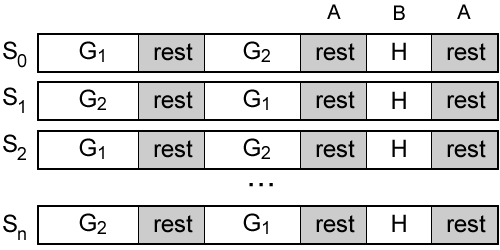
\includegraphics[width=0.6\textwidth]{figures/closing-experiment2-design.png}
%   \caption{Experimental design used in experiment 2. $S_j$ represents the $j^{\text{th}}$ subject, $G_i$ are calibration games, $COTS$ is an off-the-shelf game, and $rest$ is a resting period.}
%   \label{fig:closing-experiment2-design}
%\end{figure}

%Figure \ref{fig:closing-experiment2-design} illustrates the design of experiment 2. Each subject starts in the calibration part, where he/she plays two calibration games ($G_1$ or $G_2$) separed by a resting period (no interactions). When the subject finishes playing the calibration games, the video recordings of the subject (playing the calibration games) is processed with computer vision to extract the user signals required as input for the emotion detection model, e.g. HR and facial actions (see section \ref{sec:closing-definition-inputs}). Those extracted signals are then used to train the emotion detection model. The labeling of the signals regarding emotional states is contextualized according to the known stress and boredom aspects of the calibration games, as previously described (see sections \ref{sec:contributions} and \ref{closing:investigation-machine-learning}).

%After the model has been trained, the subject enters the emotion detection part of the experiment. In this part, the subject rests (phase A), plays a COTS game (phase B), then rests again (phase A). The video recordings of the emotion detection part is analyzed with computer vision to extract the user signals required by the emotion detection model. The extracted signals are then used as input for the previously trained emotion detection model, which outputs the estimated emotional state of the subject. The emotional state of subjects will be estimated at fixed intervals of time, e.g. every 60 seconds, throughout the emotion detection part of the experiment. Each one of those detection situations can be seen as a checkpoint. The ground truth for each checkpoint will be provided by the subjects with a self-assessment questionnaire regarding his/her current levels of stress and boredom. When a checkpoint is reached during the interaction with the COTS game, the game pauses and the questionnaire is presented to the subject. When the subject finishes answering the questionnaire, the COTS game resumes and the subject continues playing until the next checkpoint is reached.

%\begin{figure}[ht]
%    \centering
%    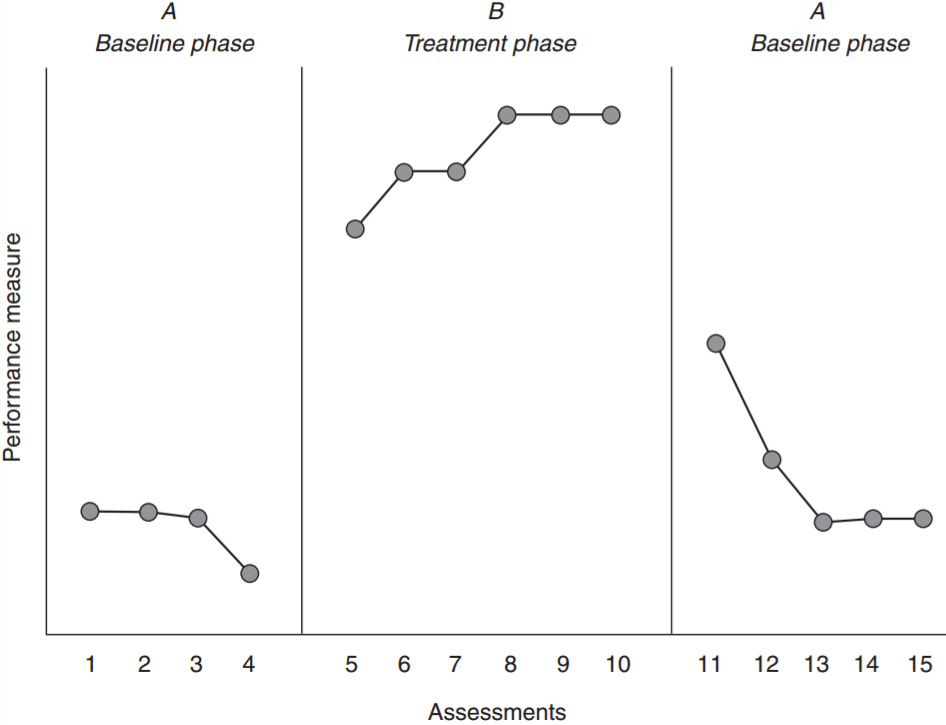
\includegraphics[width=0.85\textwidth]{figures/time-series-design-breakwell.png}
%    \caption{Time-series experimental design using an A-B-A (baseline, treatment, baseline) approach. Reproduced from \textcite{breakwell1994research}.}
%    \label{fig:time-series-design-breakwell}
%\end{figure}

%The mentioned checkpoints will be implemented using a time-series experiment design. In a time-series design there is a periodic measurement process on an individual and the introduction of a treatment into this time series of measurements results in a discontinuity in the measurements recorded in the time series \parencite{campbell2015experimental}. Figure \ref{fig:time-series-design-breakwell} illustrates the design. The A-B-A design is a common single-case time-series experimental design in which the measurements are conducted throughout the three parts of the process, i.e. A (baseline), B (treatment) and A (baseline) \parencite{robson2016real}. Phase A, referred to as the baseline phase, is a period where the subject is not under the effect of the treatment, so the measurements should reflect natural occurences. In experiment 2, it corresponds to the resting period. Phase B, referred as the treatment phase, is the period where the treatment/intervention is applied. In experiment 2, it is the interaction with the COTS game.
%In the A-B-A design, the application of a treatment followed by its removal should result in changes in the measurements among the three phases, e.g. lower values during phase A and elevated values during phase B, which confirms that the variation is a result of the treatment.

%The accuracy evaluation that confirms or refutes hypotheses \textbf{H1} and \textbf{H2} will be based on the comparison of the estimated emotional states and the self-reported emotional states informed by the subjects as ground truth during each checkpoint.

%%In the A-B-A part, the subject starts with a resting period (phase A), which is followed by the COTS treatment (phase B), finally followed by another resting period (phase A). During the A-B-A part, subjects periodically self-report their emotional state using a questionnaire, as previoslu

%%Additionally to the self-assessment of the emotional state, during the whole experiment subjects will be recorded by a video camera and monitored by a HR watch. The data collected during experiment 2 regarding the calibration games will be used to train a machine learning model, which will be used to detect the emotional state of users during the interaction with the ordinary game. The processing will be performed offline and after the experiment. Results of that analysis will prove or refute the previously mentioned hypothesis that all defined components, i.e. computer vision technique, machine learning model and calibration games, work in combination to detect emotional states.

%%During the gameplay of the non-calibration, off the shelf game the emotional state of users will be constrantly measured. Experiment 2 will produce data regarding variation of signals of subjects (from the calibration games) and ground truth data related to emotions during the gameplay of an ordinary game. The signals data will be used to train the machine learning model, which will be evaluated against the collected ground truth data (for further information regarding such validation process, see section \ref{closing:development-software}).

%%The experiment design will be based on a within-subject approach \parencite{lane2015online} where all participants perform at all levels of the treatment and there are no control groups. In the context of this research, user signals, e.g. HR, facial actions and self-reported emotional state, will be measured and used in a user-tailored model, so the division of subjects into more than one group poses a problem. Each individual will inevitably differ from one another regarding signals and emotions, such as variations in average HR during rest, for instance. Additionally people present different perceptions regarding stress and boredem. Those inherent differences pose comparision problems, so a within-subject approach simplifies the analysis of data and reduces the complexities associated with dividing subjects in different groups.

%\subsection{Challenges and unresolved issues}
%\label{experiment2-challenges}

%The first challenge regarding experiment 2 concerns the validation of the proposed method. The results of experiment 2 will demonstrate the accuracy and limitations of the proposed method, however further questioning regarding the method will innevitably surface, for instance:

%\begin{itemize}
%  \item Are all steps/signals used in the method necessary? Will a simpler and non-intrusive approach (e.g. use of remotely acquired HR information with no calibration phase) produce the same results?
%  \item Is the proposed method more accurate than an approach based on physical sensors?
%  \item Is the proposed method better than existing non-intrusive methods? It is more accurate, cheaper or easier to use?
%\end{itemize}

%Those questions could be answered with several experiments, however a direct comparison of the proposed method and existing methods is not completely plausible or viable. The proposed method relies on games as emotion elicitaion sources, which is not the case for several similar approaches that use images and sounds as stimuli. When game-like material is used as emotion elicitation sources, the context and/or the experimental design employed is different from the one proposed in experiment 2, including the use of a COTS game. Additionally a significant number of different approaches for emotion estimation exist (see chapters \ref{ch:literature-face}, \ref{ch:literature-physiological} and \ref{ch:literature-multifactorial}). Those approaches rely on different ideas, theories and signals and a direct comparison with the proposed method might not be plausible due to such differences.

%For that reason, a contextualization of the proposed method regarding existing methods is difficult. For time and resource constraints, it has been decided that an accuracy evaluation of the proposed method in comparison to a simpler emotion estimation approach based on a single signal, i.e. HR, is acceptable. It will partially answer some of the mentioned questions and provide reseachers with information to better contextualize and evaluate the feasibility of the proposed approach.

%Another challenge regarding experiment 2 is how to measure emotional states without disturbing and affecting the actual measurements. Interrupting users during gameplay is not ideal, however it is the approach described in the literature by related works. Careful planning will be required to decide the frequency and the way users will report their emotional states. If the measurements are performed too often, more data points will be available for analysis, however they might not necessarily reflect the real emotional state of users, e.g. user is bored because of the questionaire, not the game being played. If the measurements are performed too sparsely, data points will more likely reflect the real emotional state of users, however fewer data points will be available for validation.

%%Still related to emotional measurements is the decision of which questionnaire format to use in the process. As previously described, possible options are a likert scale, SAM and AS. Both SAM and AS are established and proven emotion measurement instruments, which would strengthen the theoretical foundations of the emotion measurement process. As a downside, however, they require the researcher to instruct users on how to properly answer the questionaire. User might not understand, even after the researchers explanation, what valence and arousal are, which could affect the answers and the emotion measurements. A likert scale, on the other hand, relies on the assumption that subjects know the concepts of stress and boredom within the context of games, eliminating or significantly reducing the risks of misunderstandings. If a likert scale is used, the terms ``stress" and ``boredom" can be further explained later on in the thesis using constructs of arousal and valence from established emotion theories, if that is necessary. To my understanding, a likert scale has already been successfully used in experiment 1 and is more likely to produce better results than trying to use SAM or AS as measurement tools, which risks the acquisition of answers that were misunderstood by subjects.

%Finally another unresolved issue is the COTS game to be used. Differently from the calibration games, this game should produce a natural interaction with users, causing variations of emotions that are expected from an ordinary game. The challenge is to choose a game able to elicitate sufficient variations in both boredom and stress emotional states, ortherwise the ground truth data will be skewed.

%%When measuring HR, for instance, some subjects will have higher/lower HR mean than others, independent of the group they are in or the treatment they undergo. To counter that problem, the experiment will use a one-group posttest design \cite{kirk1982experimental}, as illustrated by Figure \ref{fig:closing-experiment2-design}. Using the first row as an example, subject $S_0$ played game $G_a$ as the first level of the treatment, followed by a post-test of that game ($PT_a$), then a rest period. In the second level of the treatment, the subject played game $G_b$, followed by a post-test of that game ($PT_b$), then another rest period. Finally in the third level of the treatment, the subject played game $G_c$ followed by a post-test of that game ($PT_c$).

%%By using a one-group posttest design, each individual will perform on all levels of the treatment (play a set of different games). The within-subjects approach ensures that the differences between subjects are not interfering in the comparison, since a subject is being compared to his/herself in the different levels of the treatment. Subjects are not being compared among each other. In essence, each subject is serving as his/her own control group. According to Kirk \cite{kirk1982experimental}, the one-group posttest design should only be used when the researcher knows the mean value of the independent variable when no treatment is in effect. Such information will be obtained during the resting periods of the experiment, where the baseline value for all measured signals can be established for each subject.

%%The process of sampling a group of participants for each experiment will follow the convenience sampling approach, a non-probability sampling technique where participants are recruited because of their convenient accessibility/proximity to the researcher. Volunteers will be randomly recruited for each experiment. A probability sampling approach, where each individual of the population has an equal chance of being selected, would be ideal and would strength the external validity of the research. However the costs, logistics and time constraints associated with it makes such approach impractical in the context of this research.

\part{Outcomes and implications}
\chapter{Non-obtrusive detection of emotions}
\label{ch:discussion}

The initial chapters of this thesis presented the theoretical foundations and the work needed to create a novel method for remote detection of emotions of users during the interaction with games. As highlighted by previous research, the understanding of human emotions, as well as the process of automatically detecting them, is the aim of several researchers in a many different fields. As detailed in Chapter \ref{ch:literature-games}, different theories have been proposed to model and study emotions in a variety of contexts, including those related to games. A considerable share of those theories is based on the human physiology, connecting emotional reactions to psychophysiological signals, e.g. HR and facial activity. Several approaches have been proposed to put such models and theories into practice to achieve the ultimate goal of detecting what a person is feeling. Chapters \ref{ch:literature-face} and \ref{ch:literature-physiological}, for instance, describe the connection between emotions and their manifestations in the body, particularly the process of mapping measurable psychophysiological signals into an emotional state.

Emotion detection is a complex and multidisciplinary problem that demands knowledge from many different areas. In this thesis, focus has been given to the field of games research. This chapter presents and discusses the outcomes of this research, which is focused on creating a non-obtrusive method for emotion detection, particularly in the context of games. Results and contributions of this research are aimed at and discussed under the light of games research, however they are likely to be useful for scholars in other fields as well. The following sections also present insights obtained during the systematic investigation and development of the proposed method, including a discussion on how they relate to games research and other areas.

\section{Game-based model for emotion detection}

Commonly the process of detecting emotions using psychophysiological signals relies on mapping the patterns of such signals into an emotional state. As pointed by the literature review conducted in this thesis, a validated way of doing it is by measuring the changes of psychophysiological signals caused by the interaction between users and emotion elicitation materials. Generally the process involves three main parts: emotion elicitation, signal acquisition and the mapping of such signals into an emotional state. Simply put, subjects are exposed to materials that are likely to produce certain emotional reactions, e.g. video and images depicting sad events, followed by observations of how the signals of interest, e.g. HR, change in accordance. Finally the emotion detection is performed by a technique aimed at producing a model to map the changes of those signals into emotional states, e.g. machine learning model like neural networks. The literature review presented in this thesis shows a myriad of different approaches used in each of the previously mentioned parts.

The majority of previous work focuses on producing a group model, where data from several individuals is used to created a trained machine able to detect emotions of any other subject outside the training population. Contrary to the established notion that a group model is better, this research investigated the venue of a user-tailored approach. As pointed by previous findings \parencite{something}, a model trained on data of a given person might be better at predicting the emotional state of such person. This is motivated by the fact that people are different in many aspects, including cultural and personal expectations \parencite{some}. Furthermore it is reasonable to believe that those individual characteristics might be preserved and better accounted for in a method that uses a user-tailored model as opposed to a group model to detect emotions. In this thesis, both the emotion elicitation process and the mapping of psychophysiological signals into emotional states were focused on the notion of the individual as opposed to the group.

\subsection{Calibration games as emotion elicitation}

%When games are used, they are usually gamified version of cognitive tests, or games featuring a well defined difficulty curve, e.g. easy/hard levels. Users have different gaming skills and expectations, so a game designed to be elicitate stresss might not be perceived as such by some users.

%, while previous work explored the use of games as elicitation sources for recognizing user emotions, relying on the emotional states a person can experience \citep{mandryk2006continuous} and which physiological signals are better predictors of such states \citep{jerritta2011physiological},

Previous works have used several different emotion elicitation materials, mainly images and videos, and less often game-related elements. Those materials, however, lack a more user-tailored approach for studying the variations of signals. When games are used, emotional states such as stress and boredom are often inducted by administering a game with the same particular setup, e.g. high/low difficulty, to all subjects. People respond differently to media according to their personality \parencite{ravaja2004effects}, and they differ in social, learning and play styles \parencite{goldberg1993structure}. A game session labeled as stressful, for instance, assumes that all subjects have the same expectations and behave similarly, which dilutes the individuality of each person as some might experience the interaction as not being stressful as intended. Additionally the analysis usually involves the interaction of subjects with some game levels (from the same game) featuring a constant difficulty scale, which does not contemplate the variations of signals in a context where the game difficulty is constantly increasing in the same game level/session.

Investigation of better game-based emotion elicitation materials was one of the main aspects of this research. Aiming to properly elicitate particular emotional states on each user, this research introduced the novel idea of calibration games. As detailed in Section \ref{sec:experiment1-games-elicitation} (on page \pageref{sec:experiment1-games-elicitation}), calibration games are carefully designed and developed games that have a difficulty level that constantly and linearly progresses over time without a pre-defined stopping point. At the beginning the games are highly predictive, without novelties, changes or surprises and with emphasis on the passage of time during a wait, which leads to an emotional state of boredom \parencite{van2010behave,koster2013theory,schell2014art}. The game difficulty is then periodically increased until the subject is not able to cope with the challenges at hand, which happens at different times for different users. The ever-growing game difficulty leads to an emotional state of stress towards the end of the interaction, accounting for the different expectations and gaming skill of a wide range of users.

Sections \ref{sec:experiment1-study1} and \ref{sec:experiment1-study2} presented a detailed analysis regarding how responses of psychophysiological activity, i.e. HR and facial actions (FA), relate to emotional states in a context featuring calibration games. Results show that a calibration game is a valid emotion elicitation material which accounts for personal differences among subjects when inducing emotional states of stress and boredom. Using the proposed calibration games, it was possible to observe and confirm with statistical significance variations of HR and naked-eye recognizable FA that happened during the interactions with the games, especially under situations that were designed to provoke boredom and stress. Those findings were an essential part of the user-tailored method proposed in this thesis, since they proved that calibration games can be used as emotion elicitation material. Another important factor is the nature of the calibration games when compared to other emotional stimuli, e.g. images or videos. The use of images, videos or text as content to produce the emotional stimuli is less likely to produce the reactions of a real gaming session. In a game, users are in charge of actions, which are bound to have consequences. A bad judgment might cause the main character to get hurt, or a right movement might produce a reward. This feedback loop is happening constantly in a game, likely producing emotional reactions on the user. It is plausible to believe that the calibration games present a more sophisticated interaction through their game mechanics, as opposed to the simplistic, one-way interaction between users and images/videos, for instance. Consequentially the use of calibration games is likely to create a deeper emotional connection between users and the emotion elicitation material, resulting in clear and observable changes in psychophysiological signals.

\subsection{Remote readings of psychophysiological signals}

Several of the works found in the literature rely on physical sensors to acquire the signals used in the emotion detection model. Physical sensors are not convenient since they require a cumbersome setup and might disturb the user experience, i.e. invalidate the use of a finger or hand. Use of remote sensing to acquire psychophysiological signals, a non-obtrusive approach of data collection, is mentioned in the literature as a promising solution for that problem. Remote sensing of psychophysiological signals is an essential part of this research, since its objective is to create a method able to non-obtrusively detect user emotions. A complete non-obtrusive method for signal acquisition, however, is a complex and challenging problem, particularly in a context involving games. The literature review conducted for this thesis found the main psychophysiological signals that can be remotely acquired and whose data can be used to detect emotional states.

One of those signals that are commonly acquired using remote and non-obtrusive approaches is facial activity. Chapter \ref{ch:literature-face} (on page \pageref{ch:literature-face}) described in details techniques for facial analysis and the approaches using them for emotion detection. As mentioned in the chapter, results indicate that facial analysis is a promising source of information to be used in the process of emotion detection. Additionally  the combined use of facial and body features (multimodal emotion recognition) is known to perform better than using either one alone \parencite{zacharatos2014automatic}. Following the findings of previous work, the present thesis used facial activity as an important signal in the emotion detection process. A novel method for automated analysis of facial cues from videos was developed, as explained in Section \ref{s:experiment1-study4} (on page \pageref{s:experiment1-study4}). Empirical results of such method show its potential for detecting stress and boredom of players in games. The method is based on Euclidean distances between automatically detected facial points, designed to be robust enough to correctly perform facial analysis even when users are naturaly interacting with games. In such case, players behave naturally as they play, e.g. moving, laughing and speaking. Evaluations of the method were performed experimentally using game-based emotion elicitation, which properly contextualized the efficiency of the method in the field of games research. Results, detailed in Section \ref{s:experiment1-study4}, confirm the method has the potential to differentiate emotional states of boredom and stress of players. However the natural behavior of users during the interaction with the games is a significant factor impacting the process.

%. Secondly we present the results of an automated facial analysis performed on subjects of our experiment, who interacted with different games under boring and stressful gameplay conditions. Our results show that values of facial features detected during boring periods of gameplay are different from values of the same facial features detected during stressful periods of gameplay. Even though the nature of our games, i.e. 2D and casual, and the sample size (N=20) could be limiting factors for the generality of the evaluation of our method, we believe our population of experimental subjects is diverse and our results are still promising. Our study contributes with results that can guide further investigation regarding emotions and facial analysis in gaming contexts. .

Another signal acquired using remote and non-obtrusive approaches is HR and its derivatives. Chapter \ref{ch:literature-rppg} (on page \pageref{ch:literature-rppg}) detailed the progress that has been made in the remote estimation of physiological signals, particularly the use of rPPG to estimate HR. Despite the potential rPPG has to eliminate physical sensors completely, its use is considerably impacted by the natural behavior of users. As presented in Section \ref{s:experiment1-study3} (one page \pageref{s:experiment1-study3}), rPPG estimations of HR are sensitive to noise caused by movement, facial expressions or changes in illumination (e.g. screen activity reflected on user's face), which are all likely to happen in gaming sessions. Those interferences might produce unreliable measurements of the HR signal, resulting in misleading data. Despite those limitations, the use of remote measurement of physiological signals, such as rPPG, has already been applied to emotion detection. Signals as HR and HRV were used to remotely detect stress \parencite{mcduffcogcam, mcduff2014improvements, bousefsaf2013remote}, for instance. In the majority of the cases, subjects are typically instructed to stay still \parencite{rouast2016remote}, which improves the accuracy of the rPPG technique. In some other cases, however, authors evaluate the accuracy of the HR estimation under scenarios where subjects are instructed to act naturally. Despite the fact that such works present experiments where subjects are told to behave naturally, their accuracy evaluation is based on artificial or simple human-computer interactions. Subjects are idly staring at the camera \parencite{zhao2013remote,hsu2014learning}, faking an interaction with a computer \parencite{poh2010non}, working on a task, i.e. make a website \parencite{monkaresi2014machine} or mentally subtract numbers \parencite{mcduff2014remote}, or performing arbitrary movements \parencite{tran2015robust}, e.g. head rotation in different degrees. Differently from previous works, this thesis employed rPPG in a context where users are naturally interacting with games. Information related to HR is an important physiological indication of the emotional state of users, so the use of rPPG was essential in this thesis to remotely acquire HR data. Extensive evaluations were conducted to establish the reliability of remote HR measurements under situations with natural behavior, where users were not instructed to behave differently than what they usually do. Analysis of the accuracy of remote HR estimations clearly established the limitations of the rPPG technique, showing how it is affected by user behavior. One of those identified limitations is the effect that facial occlusion has on the rPPG estimations of the HR. The act of resting the chin on the palm of the hand, for instance, a common trait of bored users, significantly affects the process of detecting a face in the videos, thus directly affecting the estimations of HR. Evaluation results of the rPPG technique, as detailed in Section \ref{s:experiment1-study3}, have shown an average estimation error that lies within the range that still allows the identification of HR variations caused by emotion elicitation materials, as detailed in Section \ref{s:experiment1-study2}. It shows that it is feasible to remotely extract HR and facial data from video recordings of users interacting with games. As a consequence, those signals can be acquired non-obtrusively and used to detect the emotional state of users playing games.

%are presented and discussed. The main contribution of this paper is the accuracy evaluation of an established rPPG technique within the context of gaming sessions where users behave naturally instead of following movement constraint rules, e.g. remain still. Our results provide researchers with information related to the reliability of a remote HR measurement technique when applied to contexts where users behave more naturally

%is drastically impacted by noise introduced by the movement of users. Previous research countered this problem by instructing users to stand still during any interaction, or by limiting the complexity of such interactions, e.g. using images/videos as emotion elicitation materials, not games. In the present research, effort has been put to apply rPPG in a context involving users behaving naturally while interacting with games. Results

\subsection{Multifactorial emotion detection}

The literature review supporting this thesis suggests that the mapping of psychophysiological signals into emotional states based on a multifactorial analysis, when more than one signal is used, is more likely to produce accurate results \parencite{kukolja2014comparative}. As detailed in Chapter \ref{ch:literature-multifactorial}, a combination of signals can reduce the interference and noise caused by signal manipulation, enhancing the accuracy of an emotion detector. Early studies mapping psychophysiological signals into emotional states focused on a multimodal analysis, when more than one modality, e.g. ECG and skin conductivity, are used in conjunction. Such approaches use a wide variety of physical sensors to acquire signal data. As previously mentioned, physical sensors are not ideal, so a completely remote-based approach for data acquisition would be of interest.

As mentioned in Chapter \ref{ch:literature-multifactorial}, a few studies focus on remote extraction of different user signals, i.e. HR and blinking rate, from a single source, i.e. video recording. In such case, a single modality is being used, i.e. video, however a set of different signals (factors) is extracted and used in the emotion detection process, i.e. multifactorial analysis. Despite the fact that those studies use non-obtrusive extraction of user signals for emotion detection, they are not using game-focused elicitation materials. The research presented in this thesis used a novel approach to produce a multifactorial analysis, which is non-obtrusive, user-tailored and game-focused. The overall idea, presented in Section \ref{sec:research-aim} (on page \pageref{sec:research-aim}), is to remotely extract signals from a given user playing the calibration games, then use that data to train a user-tailored neural network, i.e. data from a given user is used to train a single neutral network tailored to that given user. Finally the given user, during the interaction with a particular game, i.e. ordinary, non-calibration game, has signals remotely extracted and fed into the previously trained neural network. The neural network outputs the emotional state of that given user in that particular game.

It is important to highlight that such method for emotion detection based on calibration games, remote sensing and a user-tailored multifactorial analysis has not been found in the literature. Furthermore, its feasibility was unknown and the research reported on this thesis reflects the steps taken to validate such method for emotion detection. In that light, studies 1 to 4, detailed in Sections \ref{sec:experiment1-study1} to \ref{s:experiment1-study4}, were conducted to evaluate each component of such novel emotion detection method. They focused on understanding the capabilities and limitations of each component, including their validity in the process, e.g. use of calibration games as emotion elicitation material. Each of those studies contributed to the final assembling of the novel architecture for emotion detection proposed in this thesis. Finally study 5, detailed in Sections \ref{sec:experiment1-study5} (on page \pageref{sec:experiment1-study5}), was a systematic evaluation of the feasibility of the proposed method when detecting emotions of users actually playing games. It was based on the first experiment conducted and it tested a user-tailored neural network trained on data samples from two calibration games of a given subject which was then used to classify samples from a third calibration game of that same subject. The evaluation included the testing of different user signals, such as HR and facial data combined and used separately. The intent of such evaluation was to better understand the benefits of a multifactorial analysis, confirming that it indeed produces better estimations of the emotional state of users. Results suggested that the proposed method was feasible with potential to non-obtrusively detect the emotional state of user on a user-tailored fashion during the interaction with games.

\subsection{Usage and validation}

The evaluation of feasibility of the proposed method conducted in study 5 was limited by the number of games available for analysis, i.e. three, and the reduced number of subjects. Despite those constraints, results suggested the feasibility of a non-obtrusive, game-based and user-tailored emotion detector. In order to further test such suggestions, a final validation of the proposed method was conducted in a second experiment with a larger sample size, as detailed in Chapter \ref{ch:experiment2} (on page \pageref{ch:experiment2}). In the experiment, the previously mentioned calibration games, i.e. Mushroom, Platformer and Tetris, were used as emotion elicitation materials to train a user-tailored model, i.e. neural network. Such model was then used to detect the emotional state of each user during the interaction with a fourth game, i.e. Infinite Mario. Following the expectations suggested by study 5, the proposed method was able to identify the emotional state of subjects with a mean accuracy of 61.6\%. Results confirmed with statistical significance that the proposed method indeed classified emotional states, achieving an accuracy rate better than chance-level classification.

When compared to existing works in the literature, the mean classification accuracy of 61.6\% achieved by the proposed method was still below the mean classification accuracy achieved by other affective computing studies, i.e. 77.91\%. A fair comparison of those numbers, however, is not possible. Each study is conducted in particular situations, using different emotion elicitation materials and different training/testing models. As previously mentioned, the method proposed in this thesis focuses on the individual, not on the group, which is a common factor found in the literature. Another important and highly distinctive difference between the present work and existing ones is how data is obtained to train and evaluate the emotion detection model. The method proposed in this thesis uses a completely independent dataset to train the model, which is obtained from natural interactions of users with game-focused elicitation materials, i.e. calibration games. Those games are similar to COTS games, which portrait a more real gaming experience. The evaluation of the method was conducted on the Infinite Mario game, which mimics the commercial game Super Mario. Data from such game was never seen by the trained model, yet it was able to classify the emotional state of users. As mentioned previously, the evaluation of classification performance on fresh data is a better measure for how well classifiers generalize \parencite[Chapter 5]{james2013introduction}. Several works focused on emotion detection do not use game-focused materials for training of a model. Commonly they evaluate accuracy by testings samples that are considerably similar to those found in the training dataset, e.g. splitting available data into training and evaluation datasets, which is different from what is presented in this thesis. Finally it is important to mention that the design of the proposed emotion detection method allows classifications of emotions in real-time. Stated that a user-tailored model has already been trained, the proposed method only needs an initial amount of data points before detecting emotional states, i.e. enough data to fill the moving window used for the analysis. After the minimum amount of data has been collected, e.g. 15 seconds of video data, the method can continuously estimate the emotional state of a user. The estimation can be performed with an arbitrary time interval, including for each new frame of the input video feed. Use cases, however, are more likely to employ a longer interval between classifications, e.g. 1 second, which was the value (of the windows step) used in the evaluations presented in Section \ref{s:experiment1-study5} and Chapter \ref{ch:experiment2}. Nevertheless, the proposed method is able to perform detection of emotions off line, i.e. analyze a previously recorded video, or on-line, i.e. real-time analysis of a live video streaming session.

It was unlikely that the method presented by this research, featuring several elements performing under significantly challenging situations, could outperform the accuracy achieved by over 33 affective computing studies undertaken since 1993. It is important to emphasize, however, that the systematic evaluation of the method under different studies and experiments repeatedly indicated its feasibility from statistical analysis.

 %a larger sample size and a non-calibration game.a more challenging setup  able to detect emotional states of stress and boredom in a larger scequally Following the analysis conducted in study 5, it was expected that

 %that the proposed method would still be feasible when used to detect the emotional state of users in a non-calibration.

 %Finally results suggest that a multifactorial, user-tailored model trained on data samples extracted from calibration games is a feasible method to classify emotional states of user during the interaction with games.

%Physiological signals, e.g. HR, are considered reliable sources since they are hard to fake (because of their link to the ANS), differently from facial expressions \parencite{Landowska}, for instance. When combined in the same analysis, however, those signals can complement each other and provide more information about emotional states.

\section{Insights outside games research}

Contributions of this thesis were aimed at the field of games research, however techniques and theories from a variety of fields, e.g. computer vision and psychology, were used in the investigation process. Several of the pieces that compose the proposed method for emotion detection were studied and evaluated separately, which produced insights of their own that could be used outside the field of games research.

\subsection{Facial behavior and emotions}

One of such insights relates to the exploration of facial activity under stressful and boring situations. As detailed in Section \ref{sec:experiment1-study1} (on page \pageref{sec:experiment1-study1}), observations of facial actions during the interaction with games indicate that a neutral face remains for longer periods of time during boring periods. Additionally, for the context of the experiment presented in this thesis, facial analysis on an individual level produced more information to connect facial activity to stress/boredom. Such analysis was based on an experiment with a particular configuration that allowed a better exploration of how facial activity relates to emotional states of stress and boredom. Results obtained might be used by other scholars or practitioners interested in understanding or exploring the relationship between facial activity and emotions. In that light, the present research also introduced a novel method for automated analysis of facial behavior, which has been proved to have the potential to differentiate emotional states of boredom and stress of users in real-time. Evaluations of the such automated facial analysis show that values of facial features detected during boring periods are different from values of the same facial features detected during stressful periods. Those results can contribute to further investigations regarding emotions and automated facial analysis. They could also be used as indicators of the emotional state of users in human-computer or human-robot interactions, for instance.

%This paper presented the description and results of an experiment aimed at exploring the variations of heart rate (HR) and facial actions (FA) during gaming sessions with induced boredom and stress. In total twenty adults of different ages and gaming experiences participated in the experiment, where they played three different games while being recorded by a video camera and monitored by a HR sensor. The games used in the experiment were carefully designed and implemented to have a difficulty level that linearly increases over time, from a boring to a stressful point. According to self-reported answers in post-games questionnaires, participants perceived the games as being boring at the beginning and stressful at the end.

%In the context where the measurement of physiological signals by physical and contact-based sensors is intrusive or not desired, e.g. remote estimation of HR, information from different channels is required. One of such additional channels of information might be facial expressions, such as the FA analysis performed in this paper.  We believe that this paper contributes with information regarding HR and FA in the context of games, which can be combined to create user-tailored models for emotion detection based on different data sources.

\subsection{Physiological activity and emotions}

Another insight relates to remote estimations of HR using rPPG in a context involving natural behavior. The use of rPPG is a promising technique to obtain physiological signals from users/subjects non-obtrusively. Such information has applications in research and the industry. As detailed in Section \ref{s:experiment1-study3} (on page \pageref{s:experiment1-study3}), the evaluation conducted on this thesis regarding rPPG and natural behavior provided more information related to the reliability of remote HR measurements. Even though the evaluation was performed in a context involving games, the analysis still indicates the limitations of the rPPG technique when applied on users interacting with a computer. As demonstrated, user's natural behavior, e.g. movement, affects rPPG estimations to different extents. Such information can guide the use of rPPG in contexts where the mentioned natural behavior is an inherent factor.

Finally this thesis presented an extensive analysis of how physiological signals, particularly HR, relate to emotional states of boredom and stress. As detailed in Section \ref{sec:experiment1-study2} (on page \pageref{sec:experiment1-study2}), this research presented indications that the average HR mean during periods of stress was greater than the average HR mean during periods of boredom in the interaction with games. Similarly to the facial exploration mentioned early, the analysis of the HR activity was performed in an experiment that permitted a more elaborated observation of such activity in boring and stressful interactions. Results of such analysis suggest that changes in HR is a promising indicator of stress, which contributes information to the body of knowledge of physiological reactions and emotions.

%\begin{figure}[h]
%    \centering
%    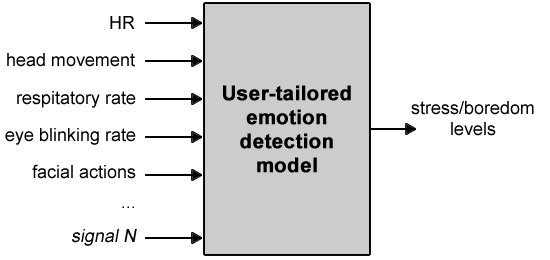
\includegraphics[width=0.6\textwidth]{figures/model-inputs-set.png}
%    \caption{Overall structure of the user-tailored emotion detection model regarding input (user signals) and output (stress/boredom levels).}
%    \label{fig:model-inputs-set}
%\end{figure}

%The user-tailored model proposed for this research might have $N$ input signals, varying from physiological ones, e.g. HR, to non-physiological ones, e.g. facial actions and head movements. Figure \ref{fig:model-inputs-set} illustrates the overall structure of the model. In order to be used in the model, an input signal needs to be supported by previous work regarding emotion detection, as well as be validated within the process of the proposed game-based calibration phase. Time and scope constraints limit the amount of input signals that can be implemented, evaluated and used in this research. As a consequence, a study will be conducted to investigate, validate and initially implement two of those signals into the proposed model: HR and facial activity (which includes head movement, lips activity, etc).

%The techniques and works presented in chapter \ref{ch:literature-face}, which relate to face detection and emotion estimation, suggest that facial analysis is an important component of a multifactorial emotion detection model. Empirical analysis of the data from the first experiment also suggest that individualities regarding facial activities do exist and could be used to estimate emotional states on a user-tailored basis \parencite{bevilacqua2016variations}. As described in section \ref{ch:literature-face-emotion-detection}, facial actions, head movement, lips/eye/mouth activity and distance measurements of detected facial landmarks are viable and proven sources of information for emotion detection.

%Regarding physiological signals, results indicate that the average HR mean for players during the last minute of gameplay is greater than the average HR mean during the second minute of gameplay (chapter \ref{ch:experiment1}, section \ref{s:experiment1-study3}). The findings are aligned with and reinforce previous research that indicates higher HR mean during stressful situations in a gaming context. The findings also suggest that changes in the HR during gaming sessions is a promising indicator of stress.

%The study will involve the definition of how those two signals will be used as inputs for the model. Facial actions, for instance, will probably be detected and measured by the euclidian distance of the facial landmarks. A vector containing the distances will be evaluated as the input for the model. Regarding the HR, its mean and standard deviation during a particular analysis window will be evaluated as input for the model. A software for the detection of those two signals will be created and used to analyse the video recordings of the first experiment (chapter \ref{ch:experiment1}). The inclusion or exclusion of a component of a signal, e.g. variations of the distances of the lips landmark points, will be based on the accuracy to detect them and the frequency they appear in boring and stressful part of the calibration games.

\chapter{Software for emotion detection}
\label{ch:software}

This chapter details the software developed to be an instanciation of the artifact produced as the outcome of this research, which is an approach for remotely detecting the changes in stress and boredom levels of a player during the interaction with a game. The software is developed in C++ and its overall structure is illustrated in Figure \ref{fig:tool-overall-structure}.

\begin{figure}[h]
    \centering
    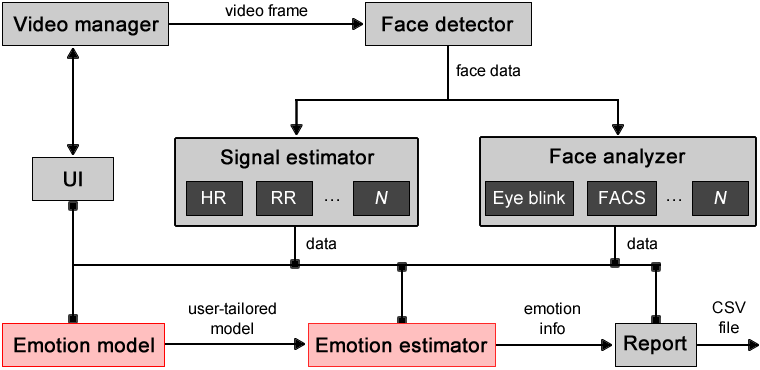
\includegraphics[width=\textwidth]{figures/tool-overall-structure.png}
    \caption{Overall structure of the software. Components highlighted in red are unfinished.}
    \label{fig:tool-overall-structure}
\end{figure}

The software contains six main components: face detector, signal estimator, face analyzer, emotion model manager, emotion estimator and finally report manager. The two components marked in read, the emotion model and the emotion estimator, are responsible for emotion estimation. Those components are unfinished and will be implemented in the future. The remaining of the components is finished and working. The following sections detail those components.

\section{Face detector}

The face detector component locates a human face in a frame of the of input video being analyzed. It performs the face alignment process using one of the two avaiable algorithms: Constrained Local Models (CLM) \parencite{cristinacce2006feature} and Ensemble of Regression Trees (ERT) \parencite{kazemi2014one}. The implementation of those techniques is provided by the OpenFace library \parencite{openface} for the former and dlib \parencite{dlib} by the latter.

\begin{figure}[h]
    \centering
    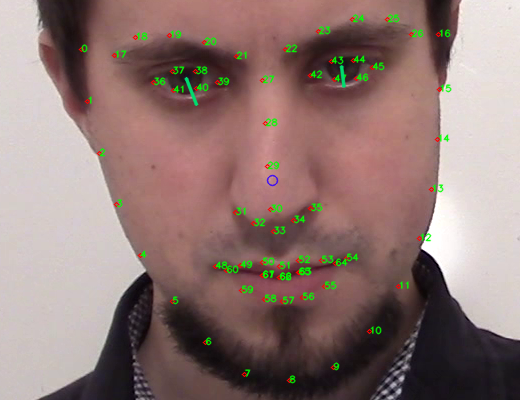
\includegraphics[width=0.8\textwidth]{figures/tool-ui-face-detector.png}
    \caption{tool-ui-face-detector}
    \label{fig:tool-ui-face-detector}
\end{figure}

The output of the face detector is a vector containing 2D points, each one representing a facial landmark. Figure \ref{fig:tool-ui-face-detector} shows a visual representation of the mentioned vector and its points.

\section{Face analyzer}

The face analyzer component uses a frame of the input video and the located face information to extract data regarding facial activity. It contains several different analyzers, each one responsible for extracting specific activity patterns, e.g. eye blink, FACS facial action units, etc. Analyzers are based on the computer vision OpenCV.

Currently the implemented analyzers extract information regarding eye area (for blinking rate), mouth area (for lips/mouth activity), facial center of mass (mean position of all detected landmarks), distance among facial landmarks, face stability (measurement of movement/rotation of the face), and head movement. Figure \ref{fig:tool-ui-face-analyzer} shows the user interface regarding the data provided by the face analyzer.

\begin{figure}[h]
    \centering
    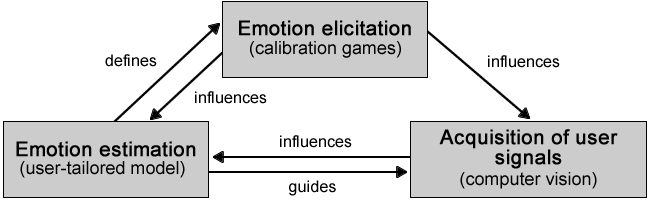
\includegraphics[width=0.8\textwidth]{figures/method-components-dependency.png}
    \caption{fig:tool-ui-face-analyzer}
    \label{fig:tool-ui-face-analyzer}
\end{figure}

\section{Signal estimator}

The signal estimator component uses the frames of the input video and the located face information to estimate user signals, e.g. HR. It contains different estimators, each one responsible for estimating a single signals. Currently two HR estimators are implemented according to the techniques by \textcite{poh2010non} and by \textcite{poh2011advancements}.

Figure \ref{fig:tool-ui-signal-estimator} shows the user interface regarding the data provided by the signal estimator.

\begin{figure}[h]
    \centering
    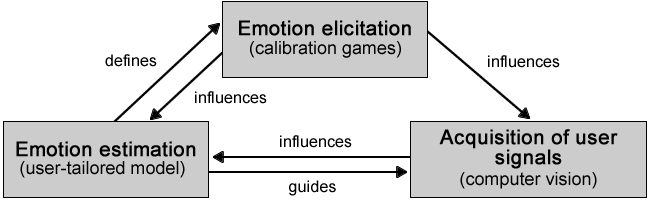
\includegraphics[width=0.8\textwidth]{figures/method-components-dependency.png}
    \caption{fig:tool-ui-signal-estimator}
    \label{fig:tool-ui-signal-estimator}
\end{figure}

\section{Report manager}

The report compoment aggregates the information produced by other components, generating a CSV report file as its output. The report files contains information regarding the video, e.g. time, as well as estimated signals and extracted facial activity. Figure \ref{fig:tool-ui-report-manager} shows part of the content of a report file.

\begin{figure}[h]
    \centering
    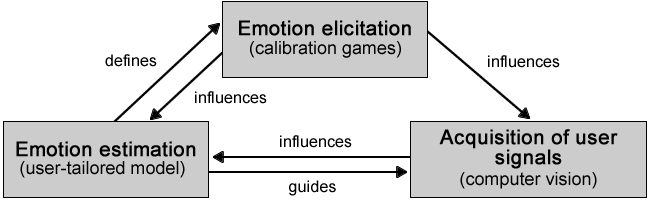
\includegraphics[width=0.8\textwidth]{figures/method-components-dependency.png}
    \caption{fig:tool-ui-report-manager}
    \label{fig:tool-ui-report-manager}
\end{figure}

\part{Closing remarks}
\chapter{Ethics and privacy}
\label{ch:ethics}

This chapter details the software developed to be an instanciation of the artifact produced as the outcome of this research, which is an approach for remotely detecting the changes in stress and boredom levels of a player during the interaction with a game.

\chapter{Conclusion}
\label{ch:conclusion}

Questionnaires and physiological measurements are the most common approach used to obtain data for emotion estimation in the field of HCI and games research. Both approaches interfere with the natural behavior of users, which affects any research procedure. Initiatives based on computer vision and remote extraction of user signals for emotion estimation exist, however they are limited. Experiments of such initiatives were performed under extremely controlled situations with few game-related stimuli. Users had a passive role with limited possibilities for interaction or emotional involvement, differently than game-based emotion stimuli, where users take an active role in the process, making decision and directly interacting with the media. Previous works also focus on predictive models based on a group perspective. As a consequece, a model is usually trained from data of several users, which in practice describes the average behavior of the group, excluding or diluting key individualities of each user. In that light, there is a lack of initiatives focusing on non-obtrusive, user-tailored emotion detection models, in particular regarding stress and boredom, within the context of games research that are based on emotion data generated from game stimuli.

This thesis proposal presented a research that aims to fill that gap, providing the HCI and the games research community with an emotion detection process, instantiated as a software tool, which can be used to remotely study users emotions in a non-obtrusive way within the context of games. Current results of this research show that individualities can be detected regarding facial activity, e.g. increased number of facial actions during the stressful part of games. Regarding physiological signals, findings are aligned with and reinforce previous research that indicate higher HR mean during stressful situations in a gaming context. The findings also suggest that changes in the HR during gaming sessions is a promising indicator of stress, which can be incorporated into a model aimed at emotion detection. As pointed out by previous work, a user-tailored model based on several signals, e.g. HR and facial activity, is more likely to detect emotional states of users.

The literature reviews, the experiments conducted so far and the planned future tasks support the idea of using a set of signals, e.g. facial activity, body movement, and HR estimations as sources of information in a multifactorial analysis for the identification of stress and boredom in games. It will produce a user-tailored approach for emotion detection focused on the behavioral particularities of each user instead of the average group pattern.

\chapter{Future work}
\label{ch:closing}

This chapter describes the plan of tasks to be performed in order to complete the proposed research aim. The tasks are related to the research objectives. Figure \ref{fig:future-work-objectives} illustrates the parts and the research objectives whose tasks will be conducted.

\begin{figure}[h]
    \centering
    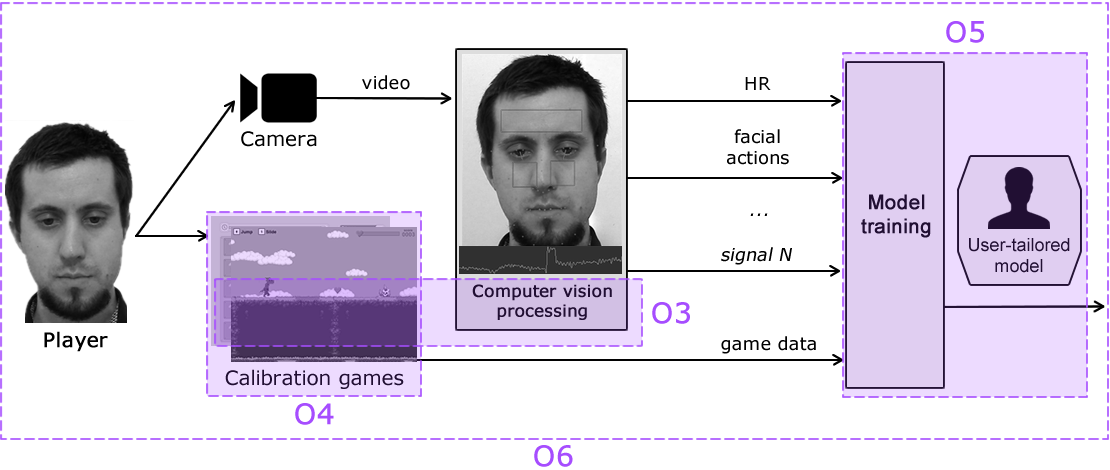
\includegraphics[width=\textwidth]{figures/future-work-objectives.png}
    \caption{Highlight of research objectives and related parts of the solution whose tasks will be conducted as future work.}
    \label{fig:future-work-objectives}
\end{figure}

The tasks involve the refinement of the process of remote acquisition of signals, definition of inputs for the user-tailored model, investigation of machine learning techniques, execution of an experiment involving emotion detection and finally the construction of a software that uses and validates the proposed method. Table \ref{tab:schedule} illustrates the schedule regarding the progression of the tasks. The following sections describe the tasks in detail.

\begin{landscape}

\begin{table}
\caption{Schedule of planned tasks}
\label{tab:schedule}
\centering
\resizebox{1.45\textwidth}{!}{%
\begin{tabular}{|p{8.3cm}|c|c|c|c|c|c|c|c|c|c|c|c|c|c|c|c|c|c|c|c|c|c|}
\hline
\textbf{Activity} & \multicolumn{8}{|c|}{2017} & \multicolumn{12}{|c|}{2018} & \multicolumn{2}{|c|}{2019} \\
\hline
& 5 & 6 & 7 & 8 & 9 & 10 & 11 & 12 & 1 & 2 & 3 & 4 & 5 & 6 & 7 & 8 & 9 & 10 & 11 & 12 & 1 & 2 \\
\hline
Refinement of remote acquisition of signals & \cellcolor{Gray} & \cellcolor{Gray} & \cellcolor{Gray} & \cellcolor{Gray} & & & & & & & & & & & & & & & & & & \\
\hline
Definition of inputs for the user-tailored model & & & & \cellcolor{Gray} & \cellcolor{Gray} & & & & & & & & & & & & &  & & & & \\
\hline
Investigation of machine learning techniques & & & & & & \cellcolor{Gray} & \cellcolor{Gray} & \cellcolor{Gray} & \cellcolor{Gray} & \cellcolor{Gray} & \cellcolor{Gray} & \cellcolor{Gray} & & & & & & & & & & \\
\hline
Experiment involving emotion detection & & & & & & & & & & & & & \cellcolor{Gray} & \cellcolor{Gray} & \cellcolor{Gray} & & & & & & & \\
\hline
Development of software to validate the approach & & & & & & & & & & & & & & & & \cellcolor{Gray} & \cellcolor{Gray} & \cellcolor{Gray} & \cellcolor{Gray} & \cellcolor{Gray} & & \\
\hline
Thesis writing & & & & \cellcolor{Gray} & & & & \cellcolor{Gray} & & & & \cellcolor{Gray} & & & \cellcolor{Gray} & \cellcolor{Gray} & \cellcolor{Gray} & \cellcolor{Gray} & \cellcolor{Gray} & \cellcolor{Gray} & & \\
\hline
Disputation & & & & & & & & & & & & & & & & & & & & & & \cellcolor{Gray} \\
\hline
\end{tabular}%
}
\end{table}

\end{landscape}

\section{Refinement of remote acquisition of signals}

The information presented in chapter \ref{ch:literature-rppg} suggests that techniques for remote extraction of physiological signals of users are significantly affected by natural behavior, e.g. head movement and facial activity. The results of the first experiment also support that, indicating that users indeed behave in a way that directly affect the accuracy of measurements. Preliminary analysis \parencite{bevilacqua2017accuracy} suggests that the accuracy of the rPPG technique is feasable under such circustances, however it is still not clear how the accuracy problems interfer with a predictive model.

As a consequence, studies will be conducted to investigate how the selected rPPG technique is affected by natural behavior of user and how it can be improved to mitigate or elimitate those problems. Figure \ref{fig:rppg-accuracy-study} illustrates the process to be conducted to evaluate and improve the accuracy of the rPPG technique.

\begin{figure}[h]
    \centering
    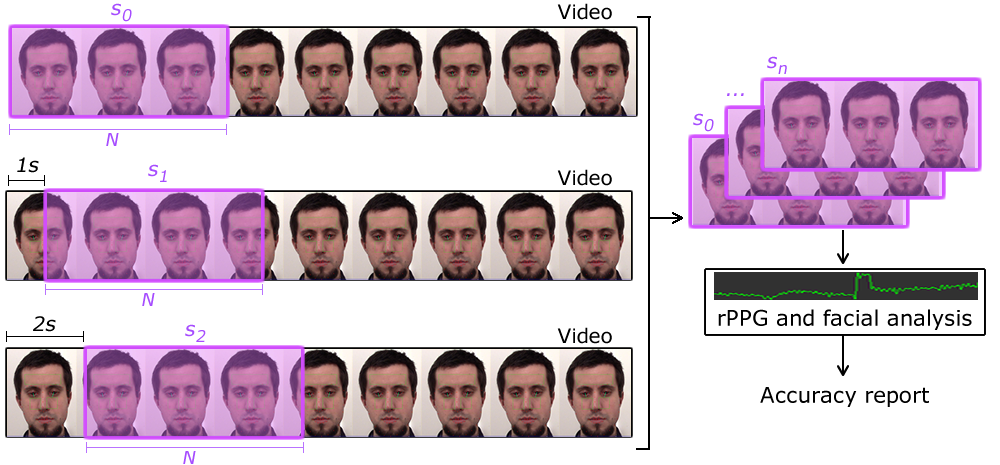
\includegraphics[width=\textwidth]{figures/rppg-accuracy-study}
    \caption{Process to evaluate the accuracy of HR estimations performed by rPPG when influenced by natural behavior.}
    \label{fig:rppg-accuracy-study}
\end{figure}

The video recordings of the first experiment will be used in the analysis. Each video will be analysed using a moving window of size $N$ seconds, which will be moved along the video with a 1 second offset, producing a set $S$ of video segments $s_i$ with $N$ seconds each. For example, assuming a 1 minute long video and a 30 seconds moving window ($N=30$), the analysis process will result in 30 $s_i$ segments ($S=30$) of 30 seconds each (0 to 30, 1 to 31, ..., 29 to 59).

Each segment $s_i$ will be used as the input for the rPPG technique for HR estimation. The estimated HR value will be compared to the average HR calculated from ground truth for the duration of the segment $s_i$. Additionally facial movement information will be calculated for each segment, such as variations of ROI size, ROI position the and variations of the central point of the detected face. Similar calculations were already conducted in study 3 (section \ref{s:study3}).

Different values for the window size $N$ will be used in the analysis, which will identify a correlation among the size of $N$, the effect of user movements and the accuracy of HR estimations. Those values will guide the adaptations proposed by previous work \parencite{li2014remote} to be applied into the selected rPPG technique to improve its accuracy within the context of this research. Examples of addaptations include the utilization of only video segments with lower subject motion, average HR estimations among different segments to infer the current HR, among others.

\section{Definition of inputs for the user-tailored model}
\label{sec:closing-definition-inputs}

The literature review presented in chapters \ref{ch:literature-physiological}, \ref{ch:literature-face} and \ref{ch:literature-multifactorial} indicates that a model based on several user signals, which is a multifactorial analysis, is more efficient for emotion detection. The mentioned chapters also highlight which of those signals can be remotely acquired within the context of this research via computer vision techniques.

\begin{figure}[h]
    \centering
    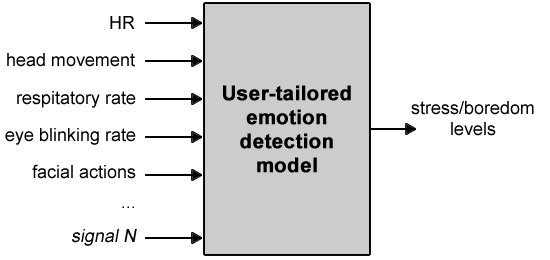
\includegraphics[width=0.6\textwidth]{figures/model-inputs-set.png}
    \caption{Overall structure of the user-tailored emotion detection model regarding input (user signals) and output (stress/boredom levels).}
    \label{fig:model-inputs-set}
\end{figure}

The user-tailored model proposed for this research might have $N$ input signals, varying from physiological ones, e.g. HR, to non-physiological ones, e.g. facial actions and head movements. Figure \ref{fig:model-inputs-set} illustrates the overall structure of the model. In order to be used in the model, an input signal needs to be supported by previous work regarding emotion detection, as well as be validated within the process of the proposed game-based calibration phase. Time and scope constraints limit the amount of input signals that can be implemented, evaluated and used in this research. As a consequence, a study will be conducted to investigate, validate and initially implement two of those signals into the proposed model: HR and facial activity (which includes head movement, lips activity, etc).

The techniques and works presented in chapter \ref{ch:literature-face}, which relate to face detection and emotion estimation, suggest that facial analysis is an important component of a multifactorial emotion detection model. Empirical analysis of the data from the first experiment also suggest that individualities regarding facial activities do exist and could be used to estimate emotional states on a user-tailored basis \parencite{bevilacqua2016variations}. As described in section \ref{ch:literature-face-emotion-prediction}, facial actions, head movement, lips/eye/mouth activity and distance measurements of detected facial landmarks are viable and proven sources of information for emotion detection.

Regarding physiological signals, results indicate that the average HR mean for players during the last minute of gameplay is greater than the average HR mean during the second minute of gameplay. The findings are aligned with and reinforce previous research that indicate higher HR mean during stressful situations in a gaming context. The findings also suggest that changes in the HR during gaming sessions is a promising indicator of stress.

The study will involve the definition of how those two signals will be used as inputs for the model. Facial actions, for instance, will probably be detected and measured by the euclidian distance of the facial landmarks. A vector containing the distances will be evaluated as the input for the model. Regarding the HR, its mean and standard variation during a particular analysis window will be evaluated as input for the model. A software for the detection of those two signals will be created and used to analyse the video recordings of the first experiment. The inclusion or exclusion of a component of a signal, e.g. variations of the distances of the lips landmark points, will be based on the accuracy to detect them and the frequency they appear in boring and stressful part of the calibration games.

\section{Investigation of machine learning techniques}
\label{closing:investigation-machine-learning}

The majority of the previous work found in the literature mention the use of machine learning techniques to model user signals into emotional states. Different models and accuracy results are mentioned, which dependent on several particularities of the approach used by the authors. A machine learning model will also be used by this research as a user-tailored emotion detection model.

\begin{figure}[h]
    \centering
    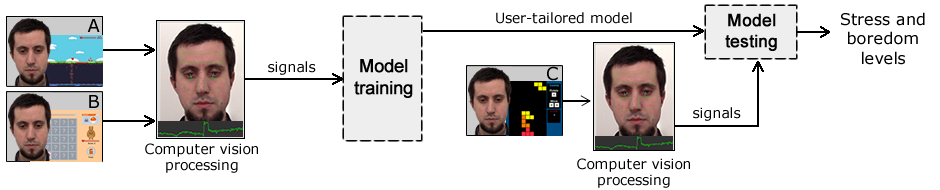
\includegraphics[width=\textwidth]{figures/machine-learning-investigation.png}
    \caption{Iteration of a 3 fold cross validation performed on the video of a gaming sessions with 3 games, i.e. A, B and C. The videos of two calibration games, e.g. A and B, are used to train the machine learning model, while the video of the third calibration game, e.g. C, is used to test the model.}
    \label{fig:machine-learning-investigation}
\end{figure}

A systematic study and accuracy evaluation will be performed to select the proper machine learning technique to be used in the model. The evaluation process will be conducted on each one of the selected (and competing) machine learning techniques using the video recordings of experiment 1. The evaluation is based on a 3 fold cross validation process, illustrated in Figure \ref{fig:machine-learning-investigation}. Initially the input signals for the emotion detection model (defined in the previous tasks, section \ref{sec:closing-definition-inputs}) will be extracted from two, e.g. A and B, of the three games played by a user and used to train the emotion detection model. The thrid game. e.g. C, that was left out of the training will be used as a testing set: user signals will be extracted from the video of that game and fed into the trained emotion detection model, which will output the predicted emotional state of the user. The 3 fold cross validation process is repeated three times, each one of them leaving out of the training phase a different game, i.e. A and B are used for training and C is used for testing, A and C are used for training and B for testing, and finally B and C are used for training and A for testing.

\begin{figure}[h]
    \centering
    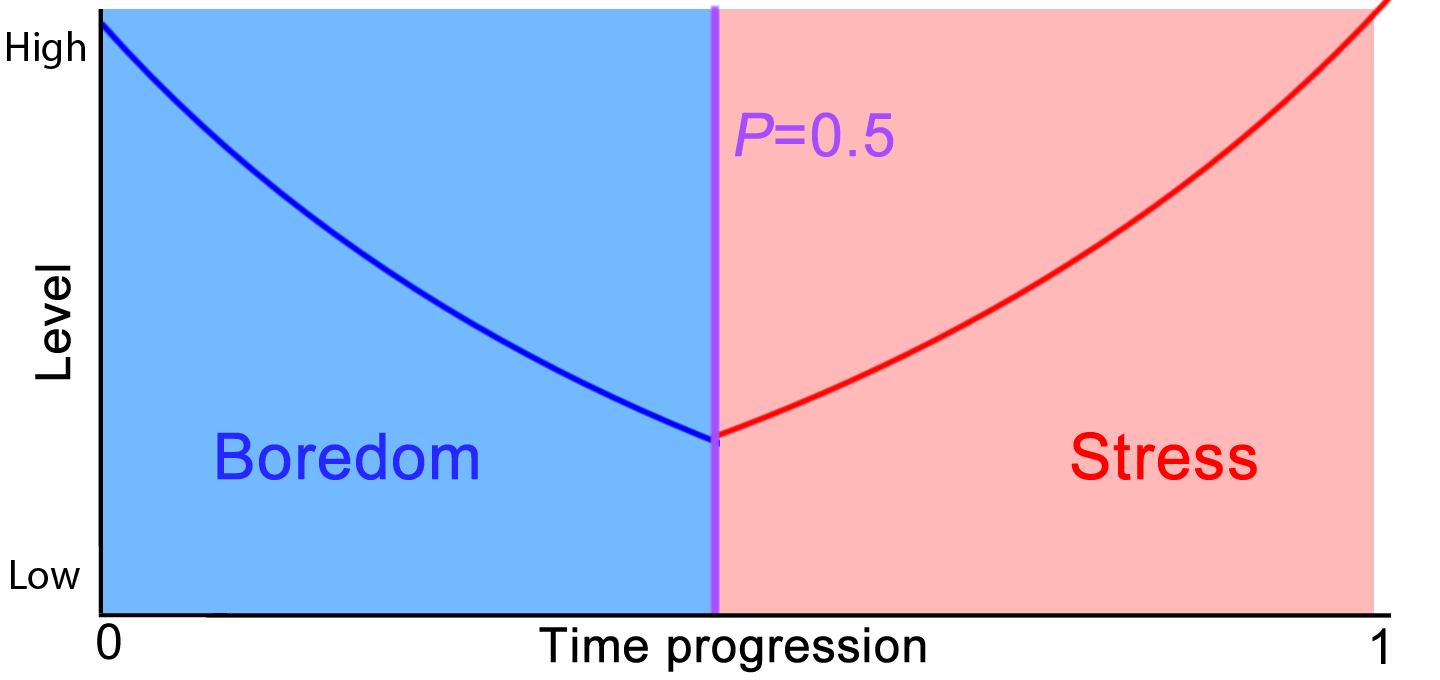
\includegraphics[width=0.8\textwidth]{figures/machine-learning-labeling-approach-A.png}
    \caption{Labeling approach for the training of the user-tailored model based on a fixed point of division $P$ for both boredom and stress samples.}
    \label{fig:machine-learning-labeling-approach-A}
\end{figure}

The video recordings that will be used in the tasks are related to experiment 1, whose games were designed to work as calibration games. As previously described in section \ref{sec:research-aim}, those calibration games feature a progression from a boring to a stressful state. That configuration will be used as the foundation for the labeling process of emotional states during the training of the model, as well as ground truth for its testing.

\begin{figure}[h]
    \centering
    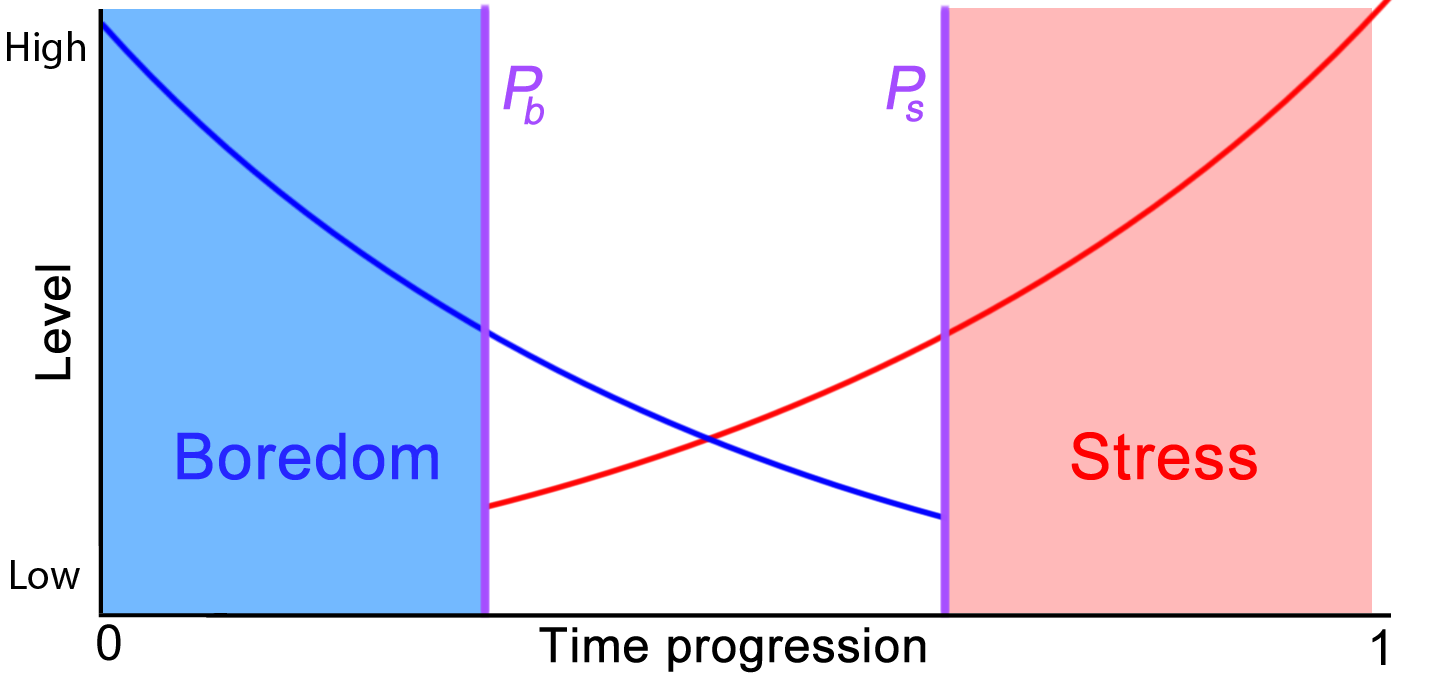
\includegraphics[width=0.8\textwidth]{figures/machine-learning-labeling-approach-B.png}
    \caption{Labeling approach for the training of the user-tailored model based on varying points of division: $P_b$ (boredom samples) and $P_s$ (stress samples).}
    \label{fig:machine-learning-labeling-approach-B}
\end{figure}

The training of the emotion detection model will be conducted according to two different strategies. In both approaches, the two games used as training sets will have their user signals sampled at a fixed interval of $T$ seconds, being $T$ empirically defined. The labeling of a sample as boredom or stress, however, will be different.

Approach \textbf{A}, illustrated in Figure \ref{fig:machine-learning-labeling-approach-A}, assumes that $P$ represents the time progression of each game, e.g. $P=0$ is the starting point of the game and $P=1$ is its end point, each game will be divided in two equal parts ($P=0.5$). Samples from the first half of the game will be labeled as boredom, while samples from the second half will be labeled as stress. The division is based on the assumption that the middle of the games accurately separates in time the self-reported perceptions of boredom and stress made by the subjects.

Approach \textbf{B}, illustrated in Figure \ref{fig:machine-learning-labeling-approach-B}, has each game divided in two parts: boredom, i.e. $P_b$, and stress, i.e. $P_s$, whose size (duration in time) will be calculated based on the self-reported answers given by subjects regarding boredom and stress. Samples from the $P_s$ part will be labeled as stress, while the samples from the $P_b$ part will be labeled as boredom. Approach \textbf{B} tries to mitigate the assumption that the middle point of the games perfectly divides the perceptions of boredom and stress. The approach accounts for the informed levels of boredom and stress of the subject, labeling only the samples within the areas more likely to accurately reflect the self-reported emotional states.

The testing process will be similar for both approaches \textbf{A} and \textbf{B}. Samples from the game used as a testing set will be collected at a fixed internal of $K$ seconds, which will be larger than $T$ and also defined empirically. The associated labeling of the samples will be based on their position according to the rules of division points, i.e. $P$, $P_b$ or $P_s$. Sample points that eventually are not labeled, e.g. middle points in approach \textbf{B}, will be labeled as neutral.

Following the described procedure, after all machine learning techniques are tested, they will have several resulting accuracy scores. The technique with the highest mean for the accuracy score will be selected. The following machine learning and classification techniques will be initially used in the tests: Support Vector Machine (SVM) using a radial basis, C-Support Vector Classification (C-SVC) using a linear kernel, K-nearest neighbours (K-nn), AdaBoost using nearest mean classifiers, Naive Bayers, and neural networks probably represented by convolution networks (convnets). Previous work also suggest a process involving decision fusion or a hierarchy of two or more classifiers working on different feature sets to improve prediction rates. Those approaches will probably be investigated as well.

\subsection{Challenges and unresolved issues}

One of the main unresolved issues regarding the use of a machine learning model is regarding its input features. Computer vision will be used to remotely extract a set of signals from the users, e.g. HR and the position of facial landmarks, however how those signals will be packeged as inputs for the machine learning model is still undefined.

The current idea is to use a direct and discrete approach where the set of extracted signals from each frame of the video being analyzed is used as is. This approach does not explicitly feed the model with information regarding the variations of the extracted signals, e.g. HR decreased 5 bpm in the last 10 seconds, instead current information from each frame is used as input, e.g. HR is 60 bpm now. The approach relies on the principle that the machine learning model will recognize any patterns regarding the variation of signals among the different samples over time, modeling those patterns as the desired mapping of emotional states.

Another possible solution is to provide the model with the variations of the signals, which demands a pre-processing of the extracted signals before feeding them into the model. In such scenario, each extracted signal will be accompanied by additional data, e.g. standard deviation, mean, etc. Ideally the machine learning model will better account for the variations of the signals and the emotional states. If a convolutional neural network is used as a machine learning solution, for instance, each signal can be used as input to the model in the form of a matrix. In that case each row of the matrix contains a segment of the signal at different times and the convnet will automatically find a way to model such changes into emotional states.

\section{Experiment involving emotion detection}
\label{closing:emotion-detection-experiment}

After the previous tasks have been completed, the limitations of the remote readings will be known (and mitigated), the set of user signals to be used in the user-tailored model will be defined and a machine learning model to map user signals into emotional states will have been selected. In summary the proposed emotion detection process will be structuraly complete, but not validated. An experiment involving emotion detection and games will then be planned and executed to validate the proposed approach.

The experiment will be similar to the first one conducted, however it will test the hypotesis that all defined components, i.e. computer vision technique, machine learning model and calibration games, work in combination to detect emotional states. The overall idea of the experiment is to make subjects play three games (two calibration games, one off the shelf game) while being recored and monitored by a HR sensor, i.e. a watch. During the gameplay of the non-calibration, off the shelf game the emotional state of users will be constrantly measured. The experiment will produce data regarding variation of signals of subjects (from the calibration games) and ground truth data related to emotions during the gameplay of an ordinary game. The signals data will be used to train the machine learning model, which will be evaluated against the collected ground truth data. The next section contains further information regarding such validation process.

The experiment design will be based on a within-subject approach \parencite{lane2015online} where all participants perform at all levels of the treatment and there are no control groups. In the context of this research, user signals, e.g. HR, facial actions and self-reported emotional state, will be measured and used in a user-tailored model, so the division of subjects into more than one group poses a problem. Each individual will inevitably differ from one another regarding signals and emotions, such as variations in average HR during rest, for instance. Additionally people present different perceptions regarding stress and boredem. Those inherent differences pose comparision problems, so a within-subject approach simplifies the analysis of data when compared to the process involving the division of subjects into different groups.

\begin{figure}[ht]
    \centering
    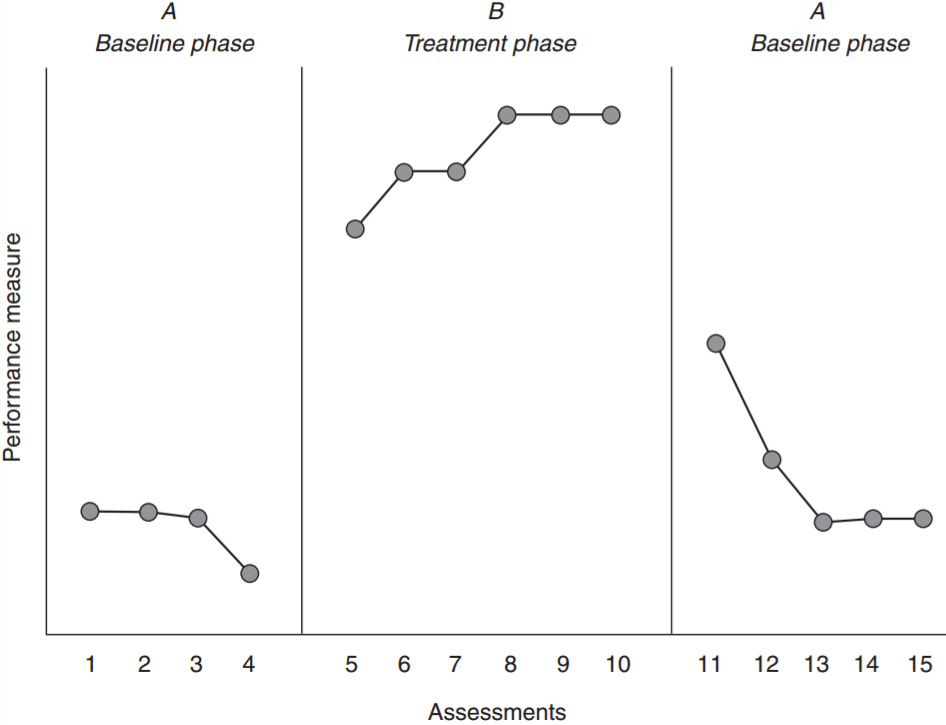
\includegraphics[width=0.85\textwidth]{figures/time-series-design-breakwell.png}
    \caption{Time-series experimental design using an A-B-A (baseline, treatment, baseline) approach. Reproduced from \textcite{breakwell1994research}.}
    \label{fig:time-series-design-breakwell}
\end{figure}

The experiment aims to validate the proposed process, so it must prove that the emotion detection process works with reasonable accuracy. As a consequence, the real emotional state of users must be known so it can be used as ground truth. In order to constantly measure the emotional state of users, a time-series experiment design will be used. In a time-series design there is a periodic measurement process on an individual and the introduction of an experimental change into this time series of measurements, which results in a discontinuity in the measurements recorded in the time series \parencite{campbell2015experimental}. Figure \ref{fig:time-series-design-breakwell} illustrates the design. The A-B-A design is a common single-case experimental design in which the measurements are conducted throughout the three parts of the experiment, i.e. A, B and A \parencite{robson2016real}. Phase A, referred to as the baseline phase, is a period where the subject is not under the effect of the treatment, so the measurements should reflect natural occurences. Phase B, referred as the treatment phase, is the period where the treatment/intervention is applied. In the A-B-A design, the application of a treatment followed by its removal should result in changes in the measurements among the three phases, e.g. lower values during phase A and elevated values during phase B, which confirms that the variation is a result of the treatment.

Figure \ref{fig:closing-experiment2-design} illustrates the design of the experiment. Procedures $G_1$ and $G_2$ will be calibration games, while treatment B will be an ordinary off the shelf game, i.e. $H$.

\begin{figure}[ht]
    \centering
    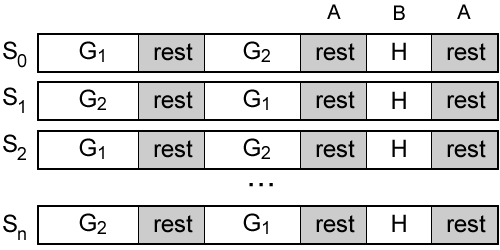
\includegraphics[width=0.6\textwidth]{figures/closing-experiment2-design.png}
    \caption{Time series experimental design used in experiment 2. $S_j$ represents the $j^{\text{th}}$ subject, $G_i$ are calibration games, $H$ is an off the shelf game, and $rest$ is a resting period.}
    \label{fig:closing-experiment2-design}
\end{figure}

The measurement regarding the level of stress and boredom of subjects will be conducted during the A-B-A phases. At fixed intervals, e.g. every 60 seconds, users will be asked to report the current emotional state. The measurement mechanism will be one of the following options (see subsection \ref{experiment2-challenges} for further discussions). A likert scale containing a question about the stress level and a question about the boredom level (approach used in experiment 1). The Self-Assessment Manikin (SAM) \parencite{morris1995observations}, which is an efficient cross-cultural measurement of emotional response regarding valence and arousal. Or the Affective Slider (AS) \parencite{betella2016affective}, a digital self-reporting tool composed of two slider controls for assessment of pleasure and arousal. Figure \ref{fig:sam-as} illustrates SAM and AS self-assessment mechanisms.

\begin{figure}[h]
\centering
  \begin{subfigure}[b]{0.5\textwidth}
    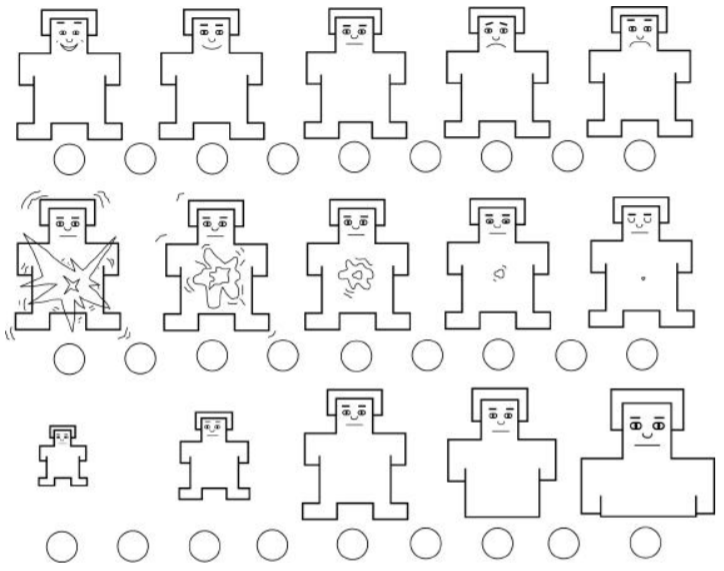
\includegraphics[width=0.95\textwidth]{figures/SAM.png}
    \caption{}
    \label{fig:sam}
  \end{subfigure}%
  \begin{subfigure}[b]{0.5\textwidth}
    \centering
    \includegraphics[width=0.95\textwidth]{figures/AS.png}
    \caption{}
    \label{fig:as}
  \end{subfigure}
  \caption{Self-reporting meaurement of emotional states. (a) Self-Assessment Manikin (SAM) \parencite{morris1995observations}; (b) Affective Slider (AS) \parencite{betella2016affective}.}
  \label{fig:sam-as}
\end{figure}

Additionally to the self-assessment of the emotional state, during the whole experiment subjects will be recorded by a video camera and monitored by a HR watch. The data collected during the experiment regarding the calibration games will be used to train a machine learning model, which will be used to detect the emotional state of users during the interaction with the ordinary game. The processing will be performed offline and after the experiment. Results of that analysis will prove or refute the previously mentioned hypothesis that all defined components, i.e. computer vision technique, machine learning model and calibration games, work in combination to detect emotional states.

\subsection{Challenges and unresolved issues}
\label{experiment2-challenges}

The first challenge regarding experiment 2 is how to measure emotional states without disturbing and affecting the actual measurements. Interrupting users during gameplay is not ideal, however it is the approach described in the literature by related works. Careful planning will be required to decide the frequency and the way users will report their emotional states. If the measurements are performed too often, more data points will be available for analysis, however they might not necessarily reflect the real emotional state of users, e.g. user is bored because of the questionaire, not the game being played. If the measurements are performed too sparsely, data points will more likely reflect the real emotional state of users, however fewer data points will be available for validation.

Still related to emotional measurements is the decision of which questionnaire format to use in the process. As previously described, possible options are a likert scale, SAM and AS. Both SAM and AS are established and proved emotion measurement instruments, which would strengthen the theoretical foundations of the emotion measurement process. As a downside, however, they require the researcher to intruct users on how to properly answer the questionaire. User might not understand, even after the researchers explanation, what valence and arousal are, which could affect the answers and the emotion measurements. A likert scale, on the other hand, relies on the assumption that subjects know the concepts of stress and boredom within the context of games, eliminating or significantly reducing the risks of misunderstandings. If a likert scale is used, the terms ``stress" and ``boredom" can be further explained later on in the thesis using terms of arousal and valence from established emotion theories, if that is necessary. To my understanding, a likert scale has already been successfully used in experiment 1 and is more likely to produce better results than trying to use SAM or AS as measurement tools, which risks the acquisition of answers that were misunderstood by subjects.

Finally another unresolved issue is the off the shelf game to be used. Differently from the calibration games, this game should produce a natural interaction with users, causing variations of emotions that are expected from an ordinary game. The challenge is to choose a game able to elicitate sufficient variations in both boredom and stress emotional states, ortherwise the ground truth data will be skewed.

%When measuring HR, for instance, some subjects will have higher/lower HR mean than others, independent of the group they are in or the treatment they undergo. To counter that problem, the experiment will use a one-group posttest design \cite{kirk1982experimental}, as illustrated by Figure \ref{fig:closing-experiment2-design}. Using the first row as an example, subject $S_0$ played game $G_a$ as the first level of the treatment, followed by a post-test of that game ($PT_a$), then a rest period. In the second level of the treatment, the subject played game $G_b$, followed by a post-test of that game ($PT_b$), then another rest period. Finally in the third level of the treatment, the subject played game $G_c$ followed by a post-test of that game ($PT_c$).

%By using a one-group posttest design, each individual will perform on all levels of the treatment (play a set of different games). The within-subjects approach ensures that the differences between subjects are not interfering in the comparison, since a subject is being compared to his/herself in the different levels of the treatment. Subjects are not being compared among each other. In essence, each subject is serving as his/her own control group. According to Kirk \cite{kirk1982experimental}, the one-group posttest design should only be used when the researcher knows the mean value of the independent variable when no treatment is in effect. Such information will be obtained during the resting periods of the experiment, where the baseline value for all measured signals can be established for each subject.

%The process of sampling a group of participants for each experiment will follow the convenience sampling approach, a non-probability sampling technique where participants are recruited because of their convenient accessibility/proximity to the researcher. Volunteers will be randomly recruited for each experiment. A probability sampling approach, where each individual of the population has an equal chance of being selected, would be ideal and would strength the external validity of the research. However the costs, logistics and time constraints associated with it makes such approach impractical in the context of this research.

\section{Development of software to validate the approach}

Following the completion of experiment 2, data regarding variations of user signals and ground truth emotional states during gameplay will be available. As previously described, the proposed emotion detection process will be structuraly complete, however not validated. The aim of this final task is to implement an instantiation of the artifact of this research, i.e. emotion detection process, as a software. The data collected during experiment 2 will be used to validate such software.

All previously described tasks involve the implementation of algorithms to remotely extract the signals and to classify them using machine learning. All those steps will be coded in Matlab to provide fast iteration and to ensure scientific valididy with previous work. The development of the software will involve the translation of all those developed parts, i.e. computer vision extraction of signals, processing of signals and mapping using machine learning, into a single and usable tool. It can be seen as an encapsulation of several individual parts, e.g. model training and emotion detection. The software will contain and orchestrate all those parts, resulting in a tool that researchers and practitioners can use for emotion detection.

The data from the calibration games of experiment 2, i.e. signal variations and video recordings, will be used to train the user-tailored model of the software. The video recordings of subjects playing the off the shelf game will be used as input for the software, which will report their detected emotional state. That information will be tested against the self-reported emotional measurements collected as ground truth during experiment 2. The results of such procedure will validate the proposed emotion detection process, producing information regarding its accuracy and limitations.

%Questionnaires and physiological measurements are the most common approach used to obtain data for emotion estimation in the field of HCI and games research. Both approaches interfere with the natural behavior of users, which affects any research procedure. Initiaties based on computer vision and remote extraction of user signals for emotion estimation exist, however they are limited. Experiments of such initiatives were performed under extremely controlled situations with few game-related stimuli. Users had a passive role with limited possibilities for interaction or emotional involvement, differently than game-based emotion stimuli, where users take an active role in the process, making decision and directly interacting with the media. Previous works also focus on predictive models based on a group perspective. As a consequece, a model is usually trained from data of several users, which in practice describes the average behavior of the group, excluding or diluting key individualities of each user. In that light, there is a lack of initiatives focusing on non-obtrusive, user-tailored emotion detection models, in particular regarding stress and boredom, within the context of games research that are based on emotion data generated from game stimuli.

%After the rPPG technique has been improved and the facial analysis has been structured, a fourth study will be conducted on the data of the first experiment. It will guide the process of refining the remote detection of physiological signals along with facial analysis, which is the foundation for the predictive model proposed in this thesis. At the present moment, the software required to perform such study is almost finished and ready to be deployed. The results of this study should lead to another publication, which will describe the improvements applied to the rPPG technique and how they affect remote estimation of physiological signals.

%\begin{appendix}
\chapter{How I Got My Appendix Removed}
\end{appendix}


%\begin{fullarticles}
%\fullarticle{bergmarklund2013gamesformaleducationalsettings}{manual.pdf}
%\end{fullarticles}

% from package 'hisbibliography'
\listofreferences

% from package 'hisbibliography'
%\dissertationlist

\end{document}
